% Modified for use with IJQC - Madhusudan Singh Copyright (C) (2011). All rights reserved.
\documentclass[12pt]{article}

\setlength{\oddsidemargin}{0in}  %left margin position, reference is one inch
\setlength{\textwidth}{6.5in}    %width of text=8.5-1in-1in for margin
\setlength{\topmargin}{-0.5in}    %reference is at 1.5in, -.5in gives a start of about 1in from top
\setlength{\textheight}{9in}     %length of text=11in-1in-1in (top and bot. marg.) 


\usepackage{amsmath,amssymb}
\usepackage{graphicx}% Include figure files
\usepackage{caption}
\usepackage{color}% Include colors for document elements
\usepackage{dcolumn}% Align table columns on decimal point
\usepackage{bm}% bold math
\usepackage[numbers,super,comma,sort&compress]{natbib}
%\usepackage[nolists, nomarkers, figuresfirst]{endfloat}

\usepackage{soul}

\definecolor{background-color}{gray}{0.98}
\graphicspath{{data/}{images/}}

%\title{Atomic pseudo-potentials for sp$^2$ carbon atoms}
\title{Atomic pseudo-potentials for reproducing $\pi$-orbital electron behaviour in sp$^2$ carbon atoms}
\author{Alexander Punter, Paola Nava, Yannick Carissan \thanks{Aix-Marseille Universit\'e, CNRS, Centrale Marseille, iSm2, Marseille, France}}

\begin{document}

\maketitle


\begin{abstract}
A pseudo-potential system for an sp\(^{2}\) carbon atom is built and tested as a building block for various pseudo-hydrocarbon chain and ring systems.  
This pseudo-system has a central charge of $Z=1$, it contains only one electron. It is employed in \textsl{ab-initio} calculations in which several physical characteristics including the orbital energies and first ionisation energy, as well as first excitation energy and UV spectra, are found to be well-reproduced by the pseudo-system. This approach is capable of reproducing the $\pi$ electron systems of small or large, planar hydrocarbons at low computational cost.
\end{abstract}

\clearpage

  \makeatletter
  \renewcommand\@biblabel[1]{#1.}
  \makeatother

\bibliographystyle{apsrev}

\renewcommand{\baselinestretch}{1.5}
\normalsize


\clearpage

%%BEGTXT
\section*{\sffamily \Large INTRODUCTION}

Since Hellmann and Gomb\'as' development of the first pseudo-potentials in the 1930s \cite{hellmann_1935, gombas_1935}, pseudo-potential methods have been employed in a variety of theoretical chemistry problems. In recent years, pseudo-potentials have been used to provide enhancements or corrections to other methods, with examples including their use as link atoms in QM/MM calculations \cite{chung_oniom_2015,
ihrig_specific_2011,
zhang_pseudobond_1998,
dilabio_simple_2002,
dilabio_efficient_2005,
gao_generalized_1998,
assfeld_quantum_1996,
jacob_calculation_2006,
von_lilienfeld_variational_2004,
von_lilienfeld_performance_2005,
von_lilienfeld_optimization_2004,
goedecker_separable_1996,
hartwigsen_relativistic_1998,
singh_combined_1986,
zhang_pseudobond_1998-1,
zhang_improved_2004,
parks_pseudobond_2008,
dilabio_simple_2002-1,
hitzenberger_optimizing_2016,
hitzenberger_probing_2015,
collins_energy-based_2015,
pezeshki_recent_2015,
von_lilienfeld_force_2013}, or the efforts to use them alongside DFT calculations in correcting for DFT errors in the effect of van der Waals forces \cite{dilabio_2008}. Their primary use, however, has always been that of increasing computational efficiency as compared with all-electron solutions for the same systems. Most well-known among these methods is the Effective Core Potential (ECP) \cite{dolg_2000}, where the replacement of core electrons in larger atoms with ECPs and RECPs (Relativistic Effective Core Potentials) permits calculations on molecules involving such atoms to be more efficient. This is not to say, however, that pseudo-potentials have been employed only in the treatment of heavy atoms. There have been efforts to create potentials for use on some lighter atoms, such as those of Topiol \emph{et al.} or Gresh and Pullman \cite{topiol_1976, gresh_1978}. 

In all of these methods, the technique has revolved around separating the electrons of an atom into core and valence electrons. We propose a different formulation. Our goal is to investigate the feasibility of pseudo-potentials reproducing electronic behaviour accurately, having been designed not only to replace the core electrons of light atoms, but also to replace specific valence electrons that do not take part in the electronic behaviour in which we are interested. Such potentials could find ready use in performing QM calculations on large hydrocarbons and polycyclic, aromatic hydrocarbons.

It is a common idea that a chemical system can be thought of as comprised of (at least) 
two parts:
an active one, where most of the chemistry takes place, and an inactive one, both of which must be taken into account in order to fulfil chemical requirements.
Based on this general statement, many successful theoretical approaches have been developed. Among them can be cited QM/QM' or QM/MM methods, fragmentation methods 
\cite{gordon_effective_2001,
steinmann_effective_2012}, and frozen core and frozen density embedding methods \cite{ASSFELD1996100, wesolowski_frozen-density_2015}.

In 1991 Huzinaga emphasised that the `dormant' electrons of the inactive region had three main effects upon the active electrons, which any pseudo-potentials should maintain; these were the Coulomb and exchange forces, as well as a `no-collapse' term \cite{huzinaga_effective_1991}.

Following his proposal, for an atom where active and dormant electrons have been separated, the Hamiltonian reads:
\begin{equation}
\label{eq:atomicHamiltonian}
\hat{H} = \sum_{i=1}^n \hat{h}(i) +\sum_{i<j}\frac{1}{r_{ij}}
\end{equation}
with $\frac{1}{r_{ij}}$ the bi-electronic interaction
between explicitly treated active electrons, and
the mono-electronic operator:
\begin{equation}
\label{eq:monoElectronicOperator}
\hat{h}(i) = -\frac{1}{2}\Delta_i - \frac{(Z-Z_c)}{r_i}+\hat{V}(i) + \hat{\sigma}(i)
\end{equation}
where $\Delta_i$ is the Laplacian of the coordinates of electron $i$, and 
$Z_C$ is the number of dormant electrons withdrawn from the reference system.
The operator $\hat{\sigma}(i)$ is the `no-collapse' term that prevents active electrons
collapsing into the dormant region. The operator $\hat{V}(i)$ reproduces the 
Coulomb and exchange interactions, for which Huzinaga proposed a spectral formulation:
\begin{equation}
\label{eq:HuzinagaMPVersion1Potential}
\hat{V} = r^{-1}\left[\sum_IA_I\exp(-\alpha_I r^2)+\sum_JB_Jr\exp(-\beta_J r^2)\right]
\end{equation}

In this article, we performed the active/inactive split on a molecule with $\pi$ electrons: the $\sigma$ electrons comprising the inactive part and the $\pi$ electrons the active part.
The Schr\"odinger equation was solved for the later part only in the field of the dormant part.
The aim is to propose a method for extracting a potential for a hybridised carbon atom 
($sp^2$), with a focus on reproducing basic properties of the electronic structure of the sp$^2$ carbon in a molecular framework 
(HOMO energy, ionisation potential and excitation energies). Our potentials can then be used as 
building blocks for constructing chemical systems, as several carbon pseudo-atoms,
each containing one explicit nuclear charge and one electron, can be connected to create extended
systems.
Moreover, the method should be usable `out of the box', in any standard quantum chemistry software
and no modification of the source code should be done.

This article is structured as follows.
In the first part, the method is defined in detail.
The second part shows the results obtained using the most refined version of the method: the extracted pseudo-potentials are then employed for extended systems, with results and discussion. A final perspective is presented in the conclusion.

\section*{\sffamily \Large METHODOLOGY}

\subsection*{\sffamily \large Choice of pseudo-potential criteria \label{section:pseudocrit}} 

Previous pseudo-potential methods have made use of different optimisation criteria, based on the pseudo-potentials' intended function. 
The pseudo-bond method, for example, is intended to facilitate geometry-optimisation in QM/MM calculations, and uses a series of reference data, 
including bond lengths and angles, across a training set of different molecules \cite{zhang_pseudobond_1998}. 
In our case, the aim is to simulate the electronic behaviour of $\pi$ systems.
Figure~\ref{figure:diagram} helps to explain our choice of criteria for gauging the efficacy of our potentials. Since our reference system is the planar CH$_3^\bullet$ radical, the HOMO energy of CH$_3^{\bullet}$, $\epsilon_{HOMO(CH_3)}$, i.e. the $p_{z}$ orbital energy, is an obvious choice, and should ensure the orbital of the pseudo-system is well-positioned to interact with other chemical moieties.

We would then take our CH$_3^{\bullet}$ pseudo-potentials and create from them a pseudo-ethylene, the smallest $\pi$ system.
In addition to the HOMO energy of the pseudo-ethylene, we decided we would also compare the $\pi-\pi^{*}$ singlet-triplet energy gap, 
and the 1$^{st}$ ionisation energy. The reproduction of the ionisation potential shows the extent to which the pseudo-system 
can still behave like the reference system upon losing an electron, whilst the $\Delta_{ST}$ ensures that the first virtual 
orbitals are well positioned, which is an indicator of the quality of the system for the reproduction of spectroscopic and 
chemical interactions.

\subsection*{\sffamily \large Pseudo-potential definition} \label{secpotdef}

As in our previous work\cite{drujon_pseudopotentials_2013},
we take the planar CH\(^{\bullet}_{3}\) as our starting system to be reproduced.
It is the smallest system containing one and only one sp$^2$ hybridised carbon atom. This choice allows us to isolate the different electrostatic interactions to build a physically meaningful model. We make use of two kinds of Gaussian pseudo-potentials, \cite{me_structure_theory} of \(s\) and \(p\) shapes. As we want to avoid modifying the quantum chemistry software itself, the pseudo-potentials have a semi-local form and we choose to preserve the \(r^{-1}\) behaviour as in Huzinaga's work.
The multi-centered pseudo-potentials that we build read as follows:
\begin{equation}
\label{eq:ourPP}
\hat{W} = r^{-1}\left[%
\underbrace{\sum_IA_I\exp(-\alpha_I r^2)\sum_m\left|Y_{1,m}\right>\left<Y_{1,m}\right|}_{\text{p projectors}}%
+%
\underbrace{\sum_JC_Jr\exp(-\gamma_J (r-r^0_J)^2)\left|Y_{0,0}\right>\left<Y_{0,0}\right|}_{\text{s projectors}}%
\right]
\end{equation}
with $Y_{0,0}$ the $s$ spherical harmonic, $Y_{1,m}$ the $p$ spherical harmonics and $r^0_J$ the relative fixed position of the $J^{th}$ potential with respect to the origin of the pseudo-atom, which carries the pseudo-potentials.
By analogy with Huzinaga model potentials defined in (\ref{eq:HuzinagaMPVersion1Potential})
we can say that the $p$ projectors aim to mimic a coulombic interaction (see the first term in Equation~\ref{eq:HuzinagaMPVersion1Potential}),
while the $s$ potentials have the task of recovering part of the bi-electronic interaction
between the dormant and the active electrons, explaining their position \textit{around} the pseudo-atom.
Thus, this second term is not stricly equivalent to Huzinaga's $B_J$ terms as our $s$ potentials aim at recovering
the bi-electronic interactions \textit{and} the no-collapse term.
This later role was devoted to the $\hat{\sigma}$ operator in Huzinaga's formulation.

Figure \ref{figure:ref_pseudo_diagram} displays the final pseudo-system: The CH\(^{\bullet}_{3}\) radical has been replaced by a hydrogen-like `pseudo-carbon', with a nuclear charge of \(Z_{nucleus} = 1\), and one electron occupying the \(p_{z}\) orbital. 
There are now no H atoms, and the system is surrounded by three potential sets at a planar distance of \(d\), each consisting of 
two \(s\)-shaped potentials with a distance above and below the \(xy\)-plane of \(c\). A further \(p\)-shaped potential is applied
directly to the pseudo-carbon.

This gives multiple variables we can use to manipulate the properties of the system.
We can alter the strength and diffuseness of the \(p\) and \(s\) potentials themselves,
as well as vary the distances \(d\) and \(c\) by moving the \(s\)-potentials.
In the effort to keep the effects 
of the $s$ potentials as localised as possible, we chose $d=0.5$ a.u. and \(c = 0.25\;a.u.\), making the atom-atom distance approximately the shortest permitted in QM programs.

Table \ref{table:potential_params} displays the data resulting from the potential extraction process. 
Initially, we optimised potentials for the CH$_3^\bullet$ system (initial pseudo).
The next step was to take two pseudo-CH\(^{\bullet}_{3}\) systems to create a pseudo-ethylene. 
This implied a refinement of the exponents and coefficients (final pseudo).
%, by fixing the \(p_{z}\) potential.
%The \(s\)-potentials are then optimised once more to give the correct HOMO energy for CH\(^{\bullet}_{3}\). We were able to optimise the first set of CH\(^{\bullet}_{3}\) potentials easily, giving us a HOMO energy exactly matching that of the reference system. 
%However, those initial pseudo-potentials lead to non-negligible errors:
%from Table \ref{table:potential_params} we see that the HOMO energy of the pseudo-system has an error of nearly 50\%. 
%We also see that our other chosen metrics, the $\Delta_{ST}$ and 1$^{st}$ ionisation energy, suffer from even greater errors. 
%We are forced to conclude that a refinement of the exponents and coefficients is necessary.
%We are forced to conclude that the assumptions made earlier in Section \ref{minimalpotguess}, that the $p_{z}$ orbital shape of CH\(^{\bullet}_{3}\) might not serve well for $C_{2}H_{4}$. This being the case, there is no reason to believe that our $Z_{eff}$ estimate, obtained from Equation \ref{equation:analyticalpz} is correct, and so our attempt at an analytical solution is no use for modelling the $\pi$ systems in which we are interested. Once we abandoned the constraints our theoretical solution placed on the potential parameters, and permitted the optimising code to find an entirely empirical solution, we were able to extract a final potential set, the results of which can be seen in Table \ref{table:potential_params}. These potentials are much better than the previous efforts, giving us a 0\% error on the $\Delta_{ST}$, and errors of 2.9\% and 7.8\% for the HOMO and 1$^{st}$ ionisation energies respectively.
In the final version of the extraction, the pseudo-ethylene system was: (1) Optimised from several different starting guesses to give the correct $\Delta_{ST}$ value. (2) The pseudo-potentials from step (1) that also gave the best HOMO and 1$^{st}$ ionisation energies were chosen as the starting guess for a final optimisation, performed by hand, to give us the final set of pseudo-potentials used in the rest of this work.
The final potential set gives an error of 5.1\% for the HOMO energy of CH\(^{\bullet}_{3}\), but it
performs much better than the initial for the ethylene,
giving us a 0.0\% error on the $\Delta_{ST}$, and errors of 2.9\% and 7.8\% for the HOMO and 1$^{st}$ ionisation energies respectively.

The potentials were extracted on the basis of Hartree-Fock calculations, but they are transferable
to other methods and they are employed within the DFT and TD-DFT frameworks in the application section (see the
computational details for further information).

\section*{\sffamily \Large RESULTS AND DISCUSSION}

%In the following subsections, the following steps are detailed: extraction of a guess pseudo-potential
%for the CH$_3^\bullet$ system, extraction of the complete set of parameters on the ethylene molecule,
%application on different larger hydrcarbons.


%\subsubsection*{\sffamily \large CH\(_{3}\): obtaining a guess for the \(s\)-potentials}
%
%We aim first at reproducing the values for the CH\(^{\bullet}_{3}\) radical as given in Table \ref{table:potential_params}. 
%This reference CH\(^{\bullet}_{3}\) is created and has its geometry optimised under Hartree-Fock (HF). 
%
%The pseudo-system is then set up, erasing the hydrogen atoms, setting the carbon charge \(Z_{nucleus} = 1\) and applying $p$ and $s$ pseudo-potentials,
%as well as selecting the correct orbital for the remaining electron.

%In order to determine the quality of the pseudo-potentials that we extract, we base our
%reasoning on Figure~\ref{figure:diagram}.
%In a first step, we focus our work on getting guess potentials, which reproduce the
%$p_z$ orbital of an sp$^2$ carbon in the field of surrounding electron pairs.
%We chose the CH$_3^\bullet$ system for that.
%This will provide us with a guess that we will use as a starting point in
%molecular frameworks were this $p_z$ orbital will be involved in $\pi$ bonds.
%Hence the $\epsilon_{HOMO(CH_3)}$ parameter is relevant to the extraction.
%
%In a second time, starting from this guess, we will optimise parameters for the smallest $\pi$
%bonded system, ethylene.
%Thus, as in this molecule more constraint apply to the $\pi$ space, we optimise
%the full set of the pseudo-potentials we have setup in order to reproduce
%$\epsilon_{HOMO}$, IP and $\Delta_{ST}$.
%As shown in Figure~\ref{figure:diagram}, these parameters allow us to fully define the energetical
%bond parameters.
%$\epsilon_{HOMO}$ ensures that the orbital should be energetically well positioned to interact
%with chemical moieties.
%The reproduction of the ionisation potential shows to what extent, the system with pseudo-potentials
%can rearrange when losing one electron.
%Finally, $\Delta_{ST}$ ensures that the first virtual orbitals are well positioned, which is an
%indicator of the quality of the system in the reproduction of spectroscopic and chemical interactions.


\subsection*{\sffamily \large Applications}

\subsubsection*{\sffamily \large C\(\mathbf{_{2n}}\)H\(\mathbf{_{2n+2}}\), \(\mathbf{2 \leq n \leq 12}\)}

Taking the final potentials we test them against a series of chain alkenes up to length C\(_{12}\)H\(_{14}\), using a variety of functionals. In each case, the geometry of the reference system is optimised according to the method used, 
before taking the reference geometry and applying the final pseudo-potentials from Table \ref{table:potential_params}. 
Figures \ref{fig:alkenes_hf_dft} and \ref{fig:alkenes_tddft} show the results. Table \ref{table:alkene_errors} gives a breakdown of the percentage errors for each method across all molecules tested. The pattern of increasing HOMO energy and decreasing cation-singlet and triplet-singlet energies seen in the reference systems is well replicated by the pseudo-alkenes, with the energies following the same gradient.

We also compare TD-DFT results for this system and results of a previous work of some of the authors, which match to within 3\%.\cite{drujon_pseudopotentials_2013}
Let us recall here that in our previous work potentials were placed at the center of bonds, which led to pseudo-potentials which were very difficult to transfer from one system to another.

\subsubsection*{\sffamily \large Large Systems}

The potentials derived above are also tested on larger systems.
Figure \ref{fig:rings_graphs} shows the $\Delta_{ST}$, the IE and
HOMO energy values for several ring systems.
As with the short chain alkenes, the general trend of the results is well-replicated
by the pseudo-systems, and the percentage errors, displayed in Table
\ref{table:ring_system_errors}, are similar.

Figure~\ref{fig:long_chain_graphs} and Table \ref{table:long_alkene_errors} refer to longer 
alkene chains (\(n\) up to 100).
The pattern of decreasing ionisation potentials and $\Delta_{ST}$ with increasing HOMO
energy is still followed, with the absolute error remaining consistent.
However, differences in the triplet-singlet energies between the reference and pseudo-systems 
become significant, notably for the largest case.

Unlike for the previous systems, there is a large discrepancy between $\Delta_{ST}$
and TD-DFT results. The pseudo-system TD-DFT results match the reference systems well, but the $\Delta_{ST}$ results do not.
The reason for this failure is to be found in the representation of the triplet state. The expectation values of the $S^2$ operator for the triplet calculations
are plotted in Figure \ref{fig:ssquare}, which shows that the spin contamination
of the triplet state computed as a single configuration (\emph{i.e.} in a SCF
framework) increases in both reference and pseudo-potential cases.
Yet, this effect is strengthened in the pseudo-potential calculations.
These results suggest that the triplet state cannot be represented as one configuration
but as a linear combination of mono-electronic excitations as done through TD-DFT.

In order to show that the recovering of the agreement between the pseudo-potential
and the reference calculations is not an artefact, we give in Table~\ref{tab:coef}
the weight and nature of each excitation (weight larger than 3\%)
in the description of the triplet excited state for
C$_{50}$H$_{52}$ (other values can be found in the SI, which exhibit the same trends).
As can be seen, the agreement is very good. 

The previous calculations show that the pseudo-potentials that we have extracted
are able to reproduce the low-lying first excited state as well as the ionisation potential
of a large range of polycyclic hydrocarbons.

Encouraged by this, we decided to explore further the virtual space by computing a large number of $\pi$ excited states, and to compare the results to reference calculations using the PBE0 functional. As can be seen from Figure~\ref{fig:cnhn_uv}, the shape of the spectra is well reproduced. We can see from the fit of the pairs of spectra that the scaling of 1.15 necessary for a near-perfect overlap is a constant throughout.
%, making it something we believe we could fix with a better optimised potential.

These results show that the pseudo-potentials that we have extracted are able to reproduce the
$\pi$ systems in a variety of situations which are not part of their extraction set.
The molecular orbital virtual space is also well described (cf. Table~\ref{tab:coef}),
which demonstrates that the good agreement with reference calculations is
physically grounded.

\subsubsection*{\sffamily \large Timings}
The model that we develop in this work allows significant computational gains.
To illustrate this, we provide in Table \ref{tab:time} a small study done on the C$_{50}$H$_{52}$
alkene chain.
Calculations were performed with two different basis sets: def2-SV(P) and QZVPPD.
When using the pseudo-potential, the basis set was truncated by removing all
basis functions not necessary to reproduce the
$\pi$ system.
In other words, only $p$ functions or those of higher angular momentum were kept.
As can be seen from Table \ref{tab:time}, the gain increases
with the size of the basis set as expected.
The gain ranges from 2.4 (def2-SV(P)) to 8 (QZVPPD).

\subsection*{\sffamily \large Physical meaning of the \(p_{z}\) pseudo-potential} \label{minimalpotguess}

The pseudo-system contains only one proton. However, the effective charge felt by the $p$ electron in a carbon atom should be larger: for instance Slater's rules suggest an effective charge of $Z_{eff}=2.4$. Thus we must account for this difference. We shall see that this role is filled by the $p$ potential once optimised. 

In order to evaluate the screening effect in the real CH\(^{\bullet}_{3}\) system, we computed the expectation value of the distance of the electron from the nucleus \( \langle r \rangle \)~:
\begin{equation}
\langle r \rangle = \langle \psi_{p_{z}} | r | \psi_{p_{z}} \rangle = 1.80\;a.u.\
\label{equation:exp_r}
\end{equation}

where \(\psi_{p_{z}}\) is the molecular orbital extracted from a reference calculation of CH\(^{\bullet}_{3}\). 

Since the CH\(^{\bullet}_{3}\) pseudo system has only one electron (as in a hydrogen-like atom), 
the analytical form of the \(p_{z}\) orbital is:~\cite{me_structure_theory} 
\begin{equation}
\label{equation:analyticalpz}
\phi_{210} = \frac{1}{\sqrt{\pi}} \frac{Z_{eff}}{2a_{0}} ^{\frac{5}{2}} re^{-\frac{Z_{eff}r}{2a_{0}}} \cos \theta
\end{equation}

where \(Z_{eff}\) is the total nuclear attraction the electron 
would feel in the real CH\(^{\bullet}_{3}\) system, taking into account the screening effect of the core electrons that would be 
present in the all-electron system.
This leads to the following expression for \( \langle r \rangle (Z_{eff}) \); 

\begin{equation}
\label{equation:PsirPsi}
\langle \phi_{210} | r | \phi_{210} \rangle = \frac{5a_{0}}{Z_{eff}}
\end{equation}

From Equations~\ref{equation:exp_r} and ~\ref{equation:PsirPsi}, we obtain the theoretical value of \(Z_{eff} = 2.77\).

The \(\psi_{p_{z}}\) molecular orbital is influenced strongly by the $p$ pseudo-potential,
because of their overlap. In this paragraph we use a simplified definition $\widehat{p}$ of the $p$ pseudo-potential, which allows for a quick evaluation of overlap effects with the basis set: 
\begin{equation}
\chi = e^{-\alpha r^{2}}\sum_{m=-1}^{+1}\left|Y_{1,m}\right>,\qquad \widehat{p} = -A | \chi \rangle \langle \chi |
\end{equation}
We define
\begin{equation}
S = \langle \psi_{p_{z}} | \chi \rangle
\end{equation}
the overlap between a molecular orbital \(\psi_{p_{z}}\), and \(\chi\),
leading us to evaluate the effect of the pseudo-potential on the \(\psi_{p_{z}}\) molecular orbital as:
\begin{equation}
\langle \psi_{p_{z}} | \widehat{p} | \psi_{p_{z}} \rangle = \langle \psi_{p_{z}} | -A | \chi \rangle \langle \chi | \psi_{p_{z}} \rangle = -A S^{2}
\end{equation}
Finally, knowing that our hydrogen-like pseudo-system already contains a charge, \(Z_{nucleus}=1\), 
we expect that:
\begin{equation}
A = (Z_{eff} - Z_{nucleus})S^{-2}
\label{eqpseudo}
\end{equation}

Ultimately, we used this expression to make informed guesses for the starting coefficients of the $p$ functions, from which we optimised the pseudo-potential.
By using Equation \ref{eqpseudo}, and the optimised exponent of $\alpha=0.624$, an estimated value of $A=3.614$ is obtained.  
The optimised coefficient $A=3.909$ of our final potential set is very close to this estimation, 
supporting the idea that the $p$ potential retrieves the incomplete screening effect of the missing electrons. 

%By using this expression and by maximising the overlap, we obtained a $p$ potential for the CH\(^{\bullet}_{3}\) system with a negative coefficient of -3.27 and an exponent of 0.30. 
%This $p$ potential, combined with the $s$ potentials, allowed us to recover the correct HOMO energy of the CH\(^{\bullet}_{3}\) system.
%It should, of course, be possible to obtain the potential parameters entirely by empirical means, but we found this reasoning gave us an informed guess at some starting parameters from which to optimise. We expected this optimisation (using the criteria described in Section \ref{section:pseudocrit}, to modify the initial values, as indeed it did. However, the final coefficient of the final $p$ pseudo-potential (-3.9) still contains this information on the incomplete screening effect of the missing electrons. 


%We now have the power to choose a \(p_{z}\) pseudo-potential solely based on the Gaussian exponent, and the \(Z_{eff}\) then follows from the above. Clearly, the exponent should be chosen to give us a strong overlap with the molecular orbital we wish to influence. Hence we arrive at a \(p_{z}\)-potential that should be physically meaningful. We chose the exponent in Table \ref{table:p_potentials}, which gave the maximum overlap possible ($\approx$ 0.79).

%\clearpage

\subsection*{\sffamily \large Computational Details}

All Hartree-Fock, DFT and time-dependent DFT (TD-DFT) energy calculations are performed with TURBOMOLE 7.1 \cite{TURBOMOLE}. The basis set used throughout is def-SV(P) \cite{defsvp}. Wherever possible, planar (C\(_{S}\)) symmetry is used. The convergence energy is \(10^{-7}\)H (\texttt{\$scfconv = 7}) for SCF and \(10^{-6}\)H for DFT. All optimisations used the Brent method in SciPy's optimisation library, with a tolerance of \(1.48*10^{-08}\), and used standard Hartree-Fock calculations.\cite{scipy}

\textbf{Chain Alkenes, Ring Molecules}. In additional to Hartree-Fock calculations, DFT is used with PBE0, PBE, TPSS and TPSSh functionals. \cite{pbe0,pbe,tpss,tpssh} The integration grid size is set at \(m4\). Also used are TD-DFT calculations, where the Tamm-Dancoff approximation (CIS) \cite{tammdancoff} is switched on to avoid triplet instability.

\section*{\sffamily \Large CONCLUSION AND PERSPECTIVE}

In this paper pseudo-potentials have been developed for sp$^{2}$-hybridised carbon units containing only one nuclear charge and one electron. 
Their main features are that: 
(1) They are fully atomic, meaning that they can be placed relative only to the carbon atom itself and the direction of its bonds. 
(2) We could show that not only were the occupied orbitals well-reproduced by the use of these new potentials, but also that the virtual space is of good quality for excited states calculation. 
They are able to reproduce basic electronic properties including HOMO, 1$^{st}$ ionisation and singlet-triplet gap energies, as well as reproduce physically reasonable absorption spectra. 
(3) They can be employed with both Hartree-Fock and DFT methods including PBE0, PBE, TPSS and TPSSh functionals. 
(4) They have been shown to function well whether their neighbouring atoms are other pseudo-carbons (as with fused carbon rings), hydrogen atoms (as in CH\(^{\bullet}_{3}\)), or a mixture of both (as in the chain alkenes or at the edge of fused ring systems). 
(5) They offer a significant gain in computational time as compared to all-electron calculations.

Our work remains ongoing, and we envisage two areas for further development (1) We would like to create potentials that can successfully interact with neighbouring all-electron atoms. This will mean producing potentials which are capable of bonding covalently with their neighbours, i.e. adding another electron to the pseudo-carbon for every bonding, all-electron neighbouring atom. Such potentials could be useful as link atoms in QM/MM calculations, functioning similarly to Quantum Capping Potentials \cite{dilabio_simple_2002}, though this is not our primary motivation. (2) We would like further to test and to expand this work into a general method for increasing computational efficency in large systems in which there are many sp$^{2}$ carbon units, both in SCF calculations and the generation of electronic spectra. This could be particularly useful in large molecules which are optically active, such as helicenes, to simulate ECD spectra.

\clearpage

%%%%%%%%%%%%%%%%%%%%%%%%%%%%%%%%%%%%%%%%%%%%%%%%%%%%%%%%%%%%%%%%%%%%%%%%%%%%%%%%%
% BIBLIOGRAPHY

\bibliography{biblio_pseudo_alex}   % Produces the bibliography via BibTeX.
%%ENDTXT

%\begin{thebibliography}{99}
%
%
%\bibitem{Coulson}
%Coulson, C. A., Rev. Mod. Phys., \textbf{1960}, 32,170-177.
%\bibitem{Malrieu}
%Malrieu, J.-P., J. Mol. Struct., \textbf{1998}, 424, 1-2,83-91.
%\bibitem{Shaik}
%Shaik, S., New. J. Chem., \textbf{2007}, 31,2015-2028.
%\bibitem{Hoffmann}
%Hoffman, R., Schleyer, P. v. R., Schaefer III, H. F., \textbf{2008}, 47, 7164-7167.
%\bibitem{Perdew}
%Perdew, J. P., Ruzsinszky, A., Constantin, L., Sun, J., Csonka, G., J. Chem. Theory Comput., \textbf{2009}, 5, 902-908.
%\bibitem{Koros}
%Koros, W. J.; Chern, R. T. In Handbook of Separation Process Technology; Rousseau, E. D.; Russell, B., Eds.; Wiley: New York, \textbf{1987}; Vol. 2, Chapter 20, pp 34-45.
%\end{thebibliography}


%%%%%%%%%%%%%%%%%%%%%%%%%%%%%%%%%%%%%%%%%%%%%%%%%%%%%%%%%%%%%%%%%%%%%%%%%%%%%%%%%

\clearpage
%%%%%%%%%%%%%%%%%%%%%%%%%%%%%%%%%%%%%%%%%%%%%%%%%%%%%%%%%%%%%%%%%%%%%%%%%%%%%%%%%
% FIGURE CAPTIONS

%BEGFIG
\begin{figure}
%\vspace*{0.1in}   %%% FIGURE 0
\begin{center}

\includegraphics[width=\columnwidth]{diagram.png}
\end{center}
\vspace{0.25in}
\hspace*{3in}
	\caption{Definition of the criteria chosen to optimize the pseudo-potentials
	(IP: ionisation potential, $\Delta_{ST}$: singlet-triplet excitation energy, $\epsilon_{HOMO}$: energy of the HOMO orbital).
	IP allow the inclusion of the relaxation of the orbitals when the system is ionised, whereas $\epsilon_{HOMO}$ is more important
	in a chemical framework.}
\label{figure:diagram}
\end{figure}

%%%%% FIGURE ---- cc.eps
\begin{figure}
%\vspace*{0.1in}   %%% FIGURE 1
\begin{center}
%\includegraphics[width=0.2\columnwidth,keepaspectratio=true]{cc.eps}
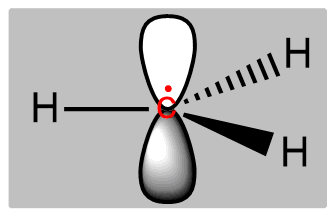
\includegraphics[width=8cm]{ch3.png}
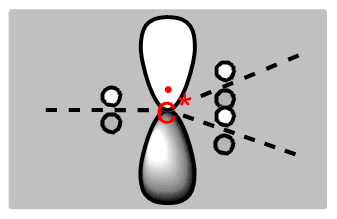
\includegraphics[width=8cm]{pseudoch3.png}
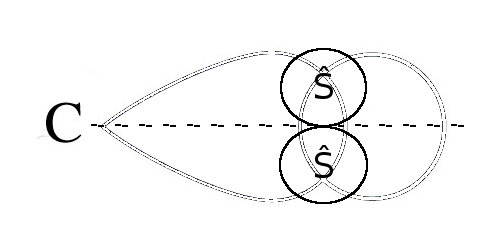
\includegraphics[width=8cm]{tm_sp2_potentials.png}
%\caption{Diagrams of CH\(^{\bullet}_{3}\) (left) and pseudo-CH\(^{\bullet}_{3}\) (right, below) molecules. The pseudo-CH\(^{\bullet}_{3}\) diagrams display the \(s\) and \(p\)-potential positions, and the distances \(d\) and \(c\).}
%\label{figure:ref_pseudo_diagram}
\end{center}
\vspace{0.25in}
\hspace*{3in}
\caption{Diagrams of CH\(^{\bullet}_{3}\) (left) and pseudo-CH\(^{\bullet}_{3}\) (right, below) molecules. The pseudo-CH\(^{\bullet}_{3}\) diagrams display the \(s\) and \(p\)-potential positions, and the distances \(d\) and \(c\).}
\label{figure:ref_pseudo_diagram}
\end{figure}

%\begin{figure}
%%\vspace*{0.1in}   %%% FIGURE 2
%\begin{center}
%%\includegraphics[width=0.2\columnwidth,keepaspectratio=true]{cc.eps}
%\fbox{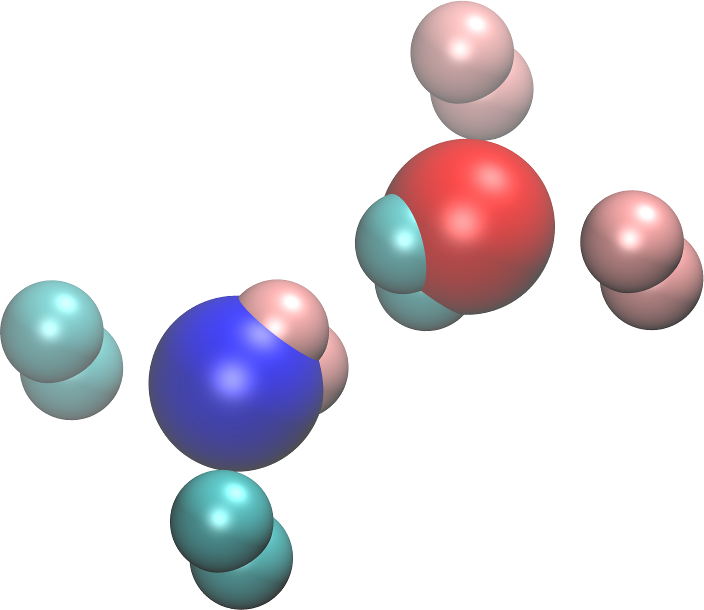
\includegraphics[width=0.45\textwidth]{hires_long_r_crop.png}}%
%\fbox{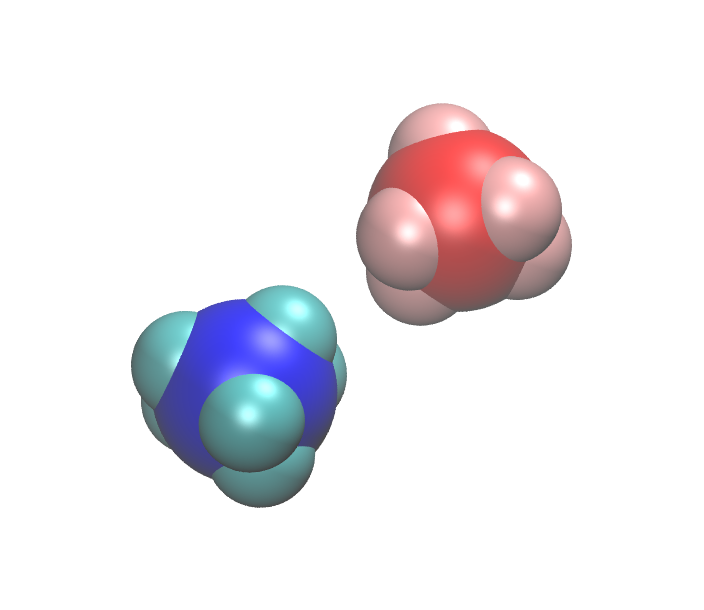
\includegraphics[width=0.45\textwidth]{hires_short_r_crop.png}}
%%\caption{Diagrams of pseudo-ethene with \(d =\) 2.0 a.u. (left), and \(d = 0.5\) a.u. (right). The first pseudo-carbon is displayed in blue, with its \(s\) pseudo-potentials in cyan, and the second pseudo-carbon is in red, with its potentials in pink.}
%%\label{fig:long_r_ethene}
%\end{center}
%\vspace{0.25in}
%\hspace*{3in}
%
%\caption{Diagrams of pseudo-ethene with \(d =\) 2.0 a.u. (left), and \(d = 0.5\) a.u. (right). The first pseudo-carbon is displayed in blue, with its \(s\) pseudo-potentials in cyan, and the second pseudo-carbon is in red, with its potentials in pink.}
%\label{fig:long_r_ethene}
%\end{figure}

\begin{figure}
%\vspace*{0.1in}   %%% FIGURE 3
\begin{center}
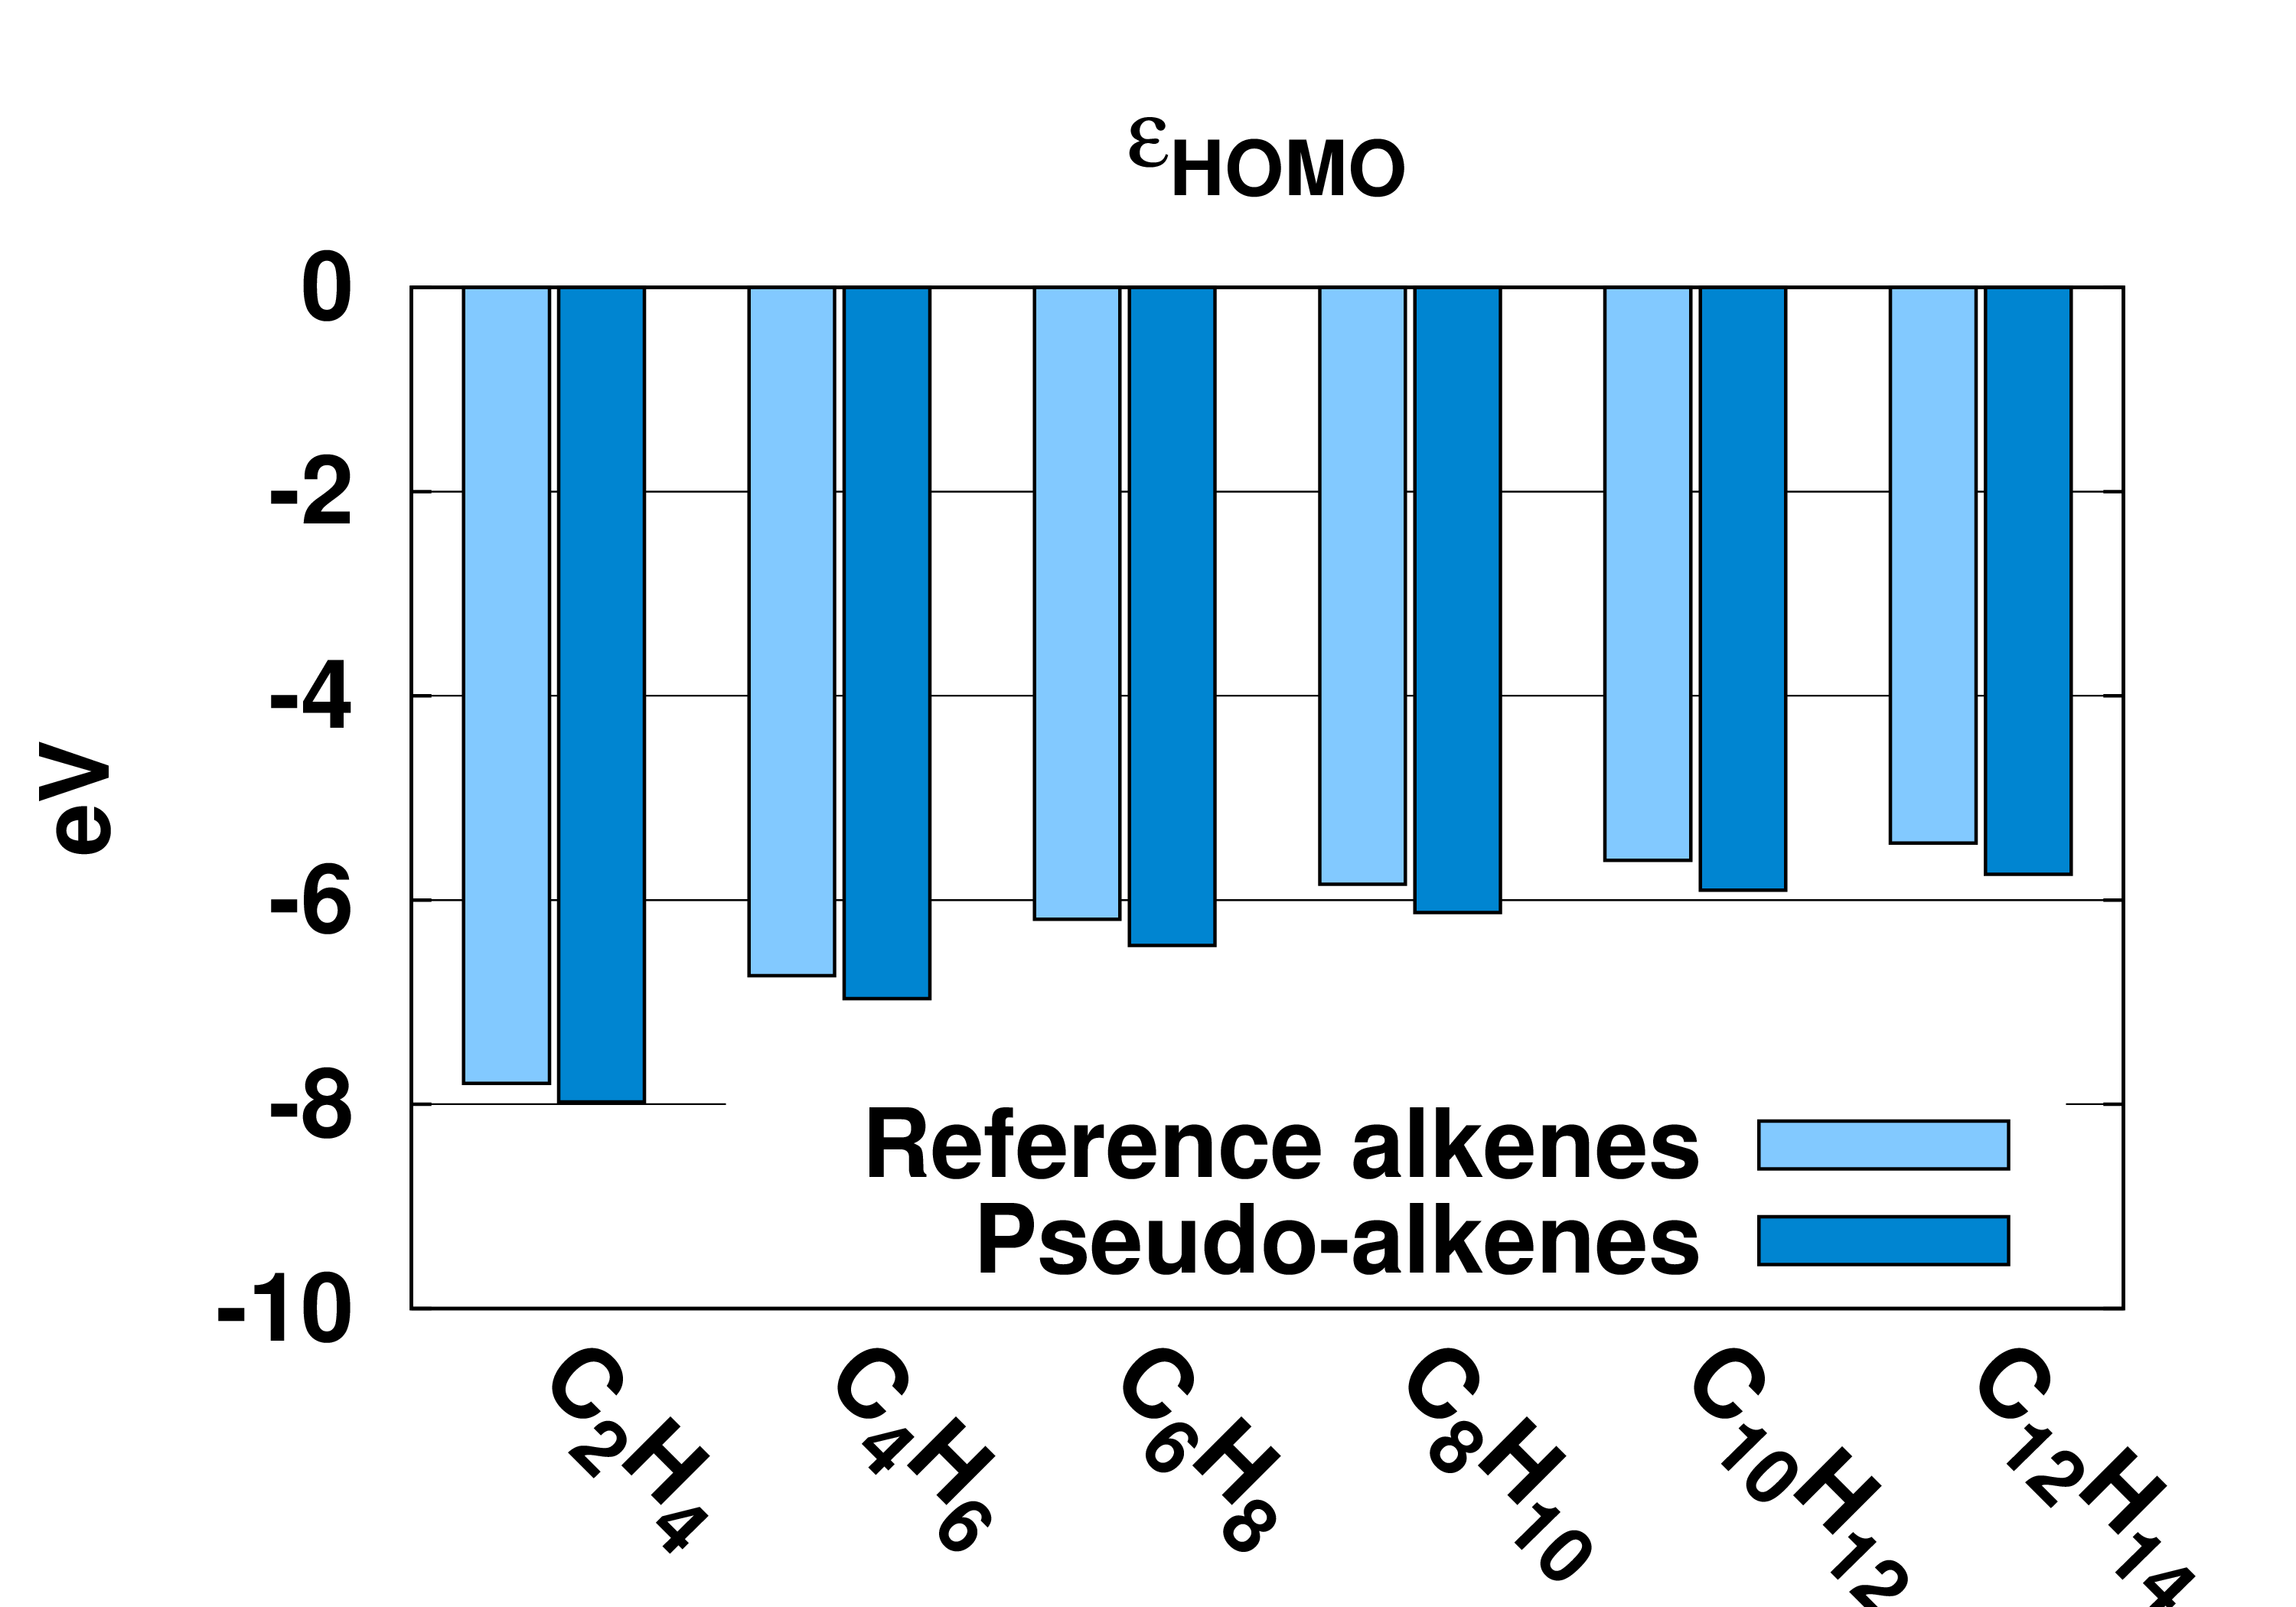
\includegraphics[width=8cm]{short_pbe0_homo}
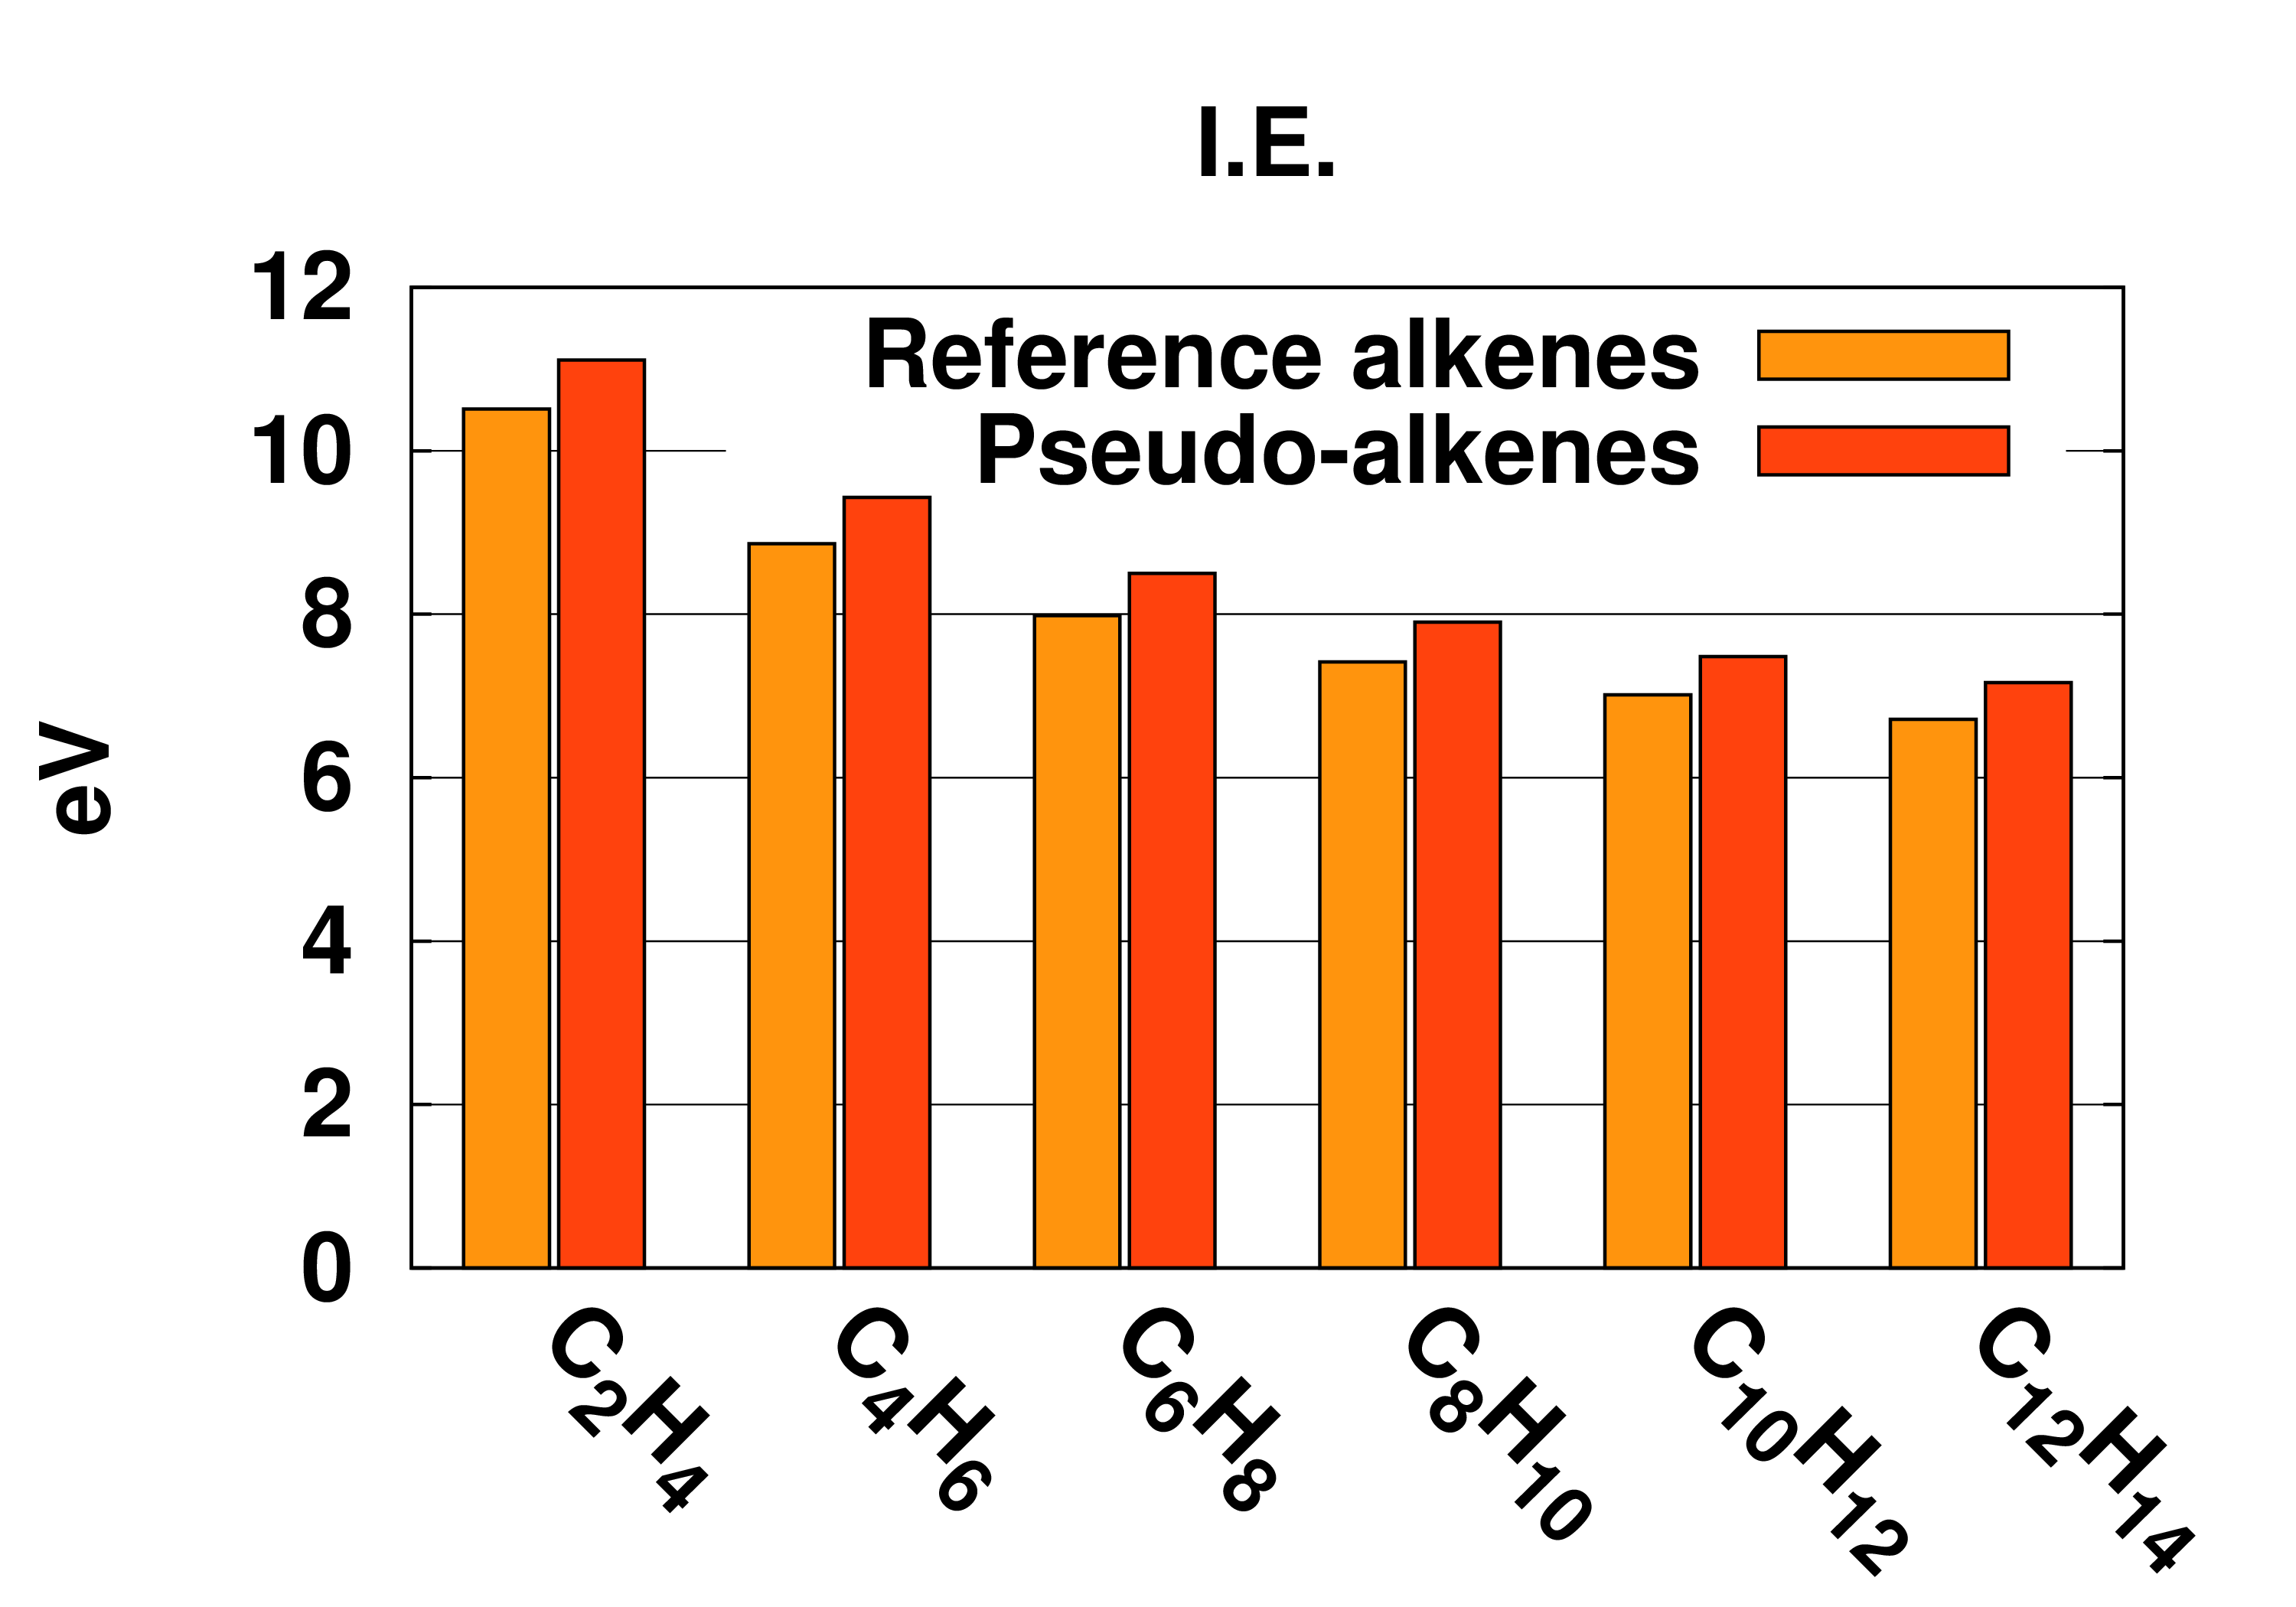
\includegraphics[width=8cm]{short_pbe0_ie}
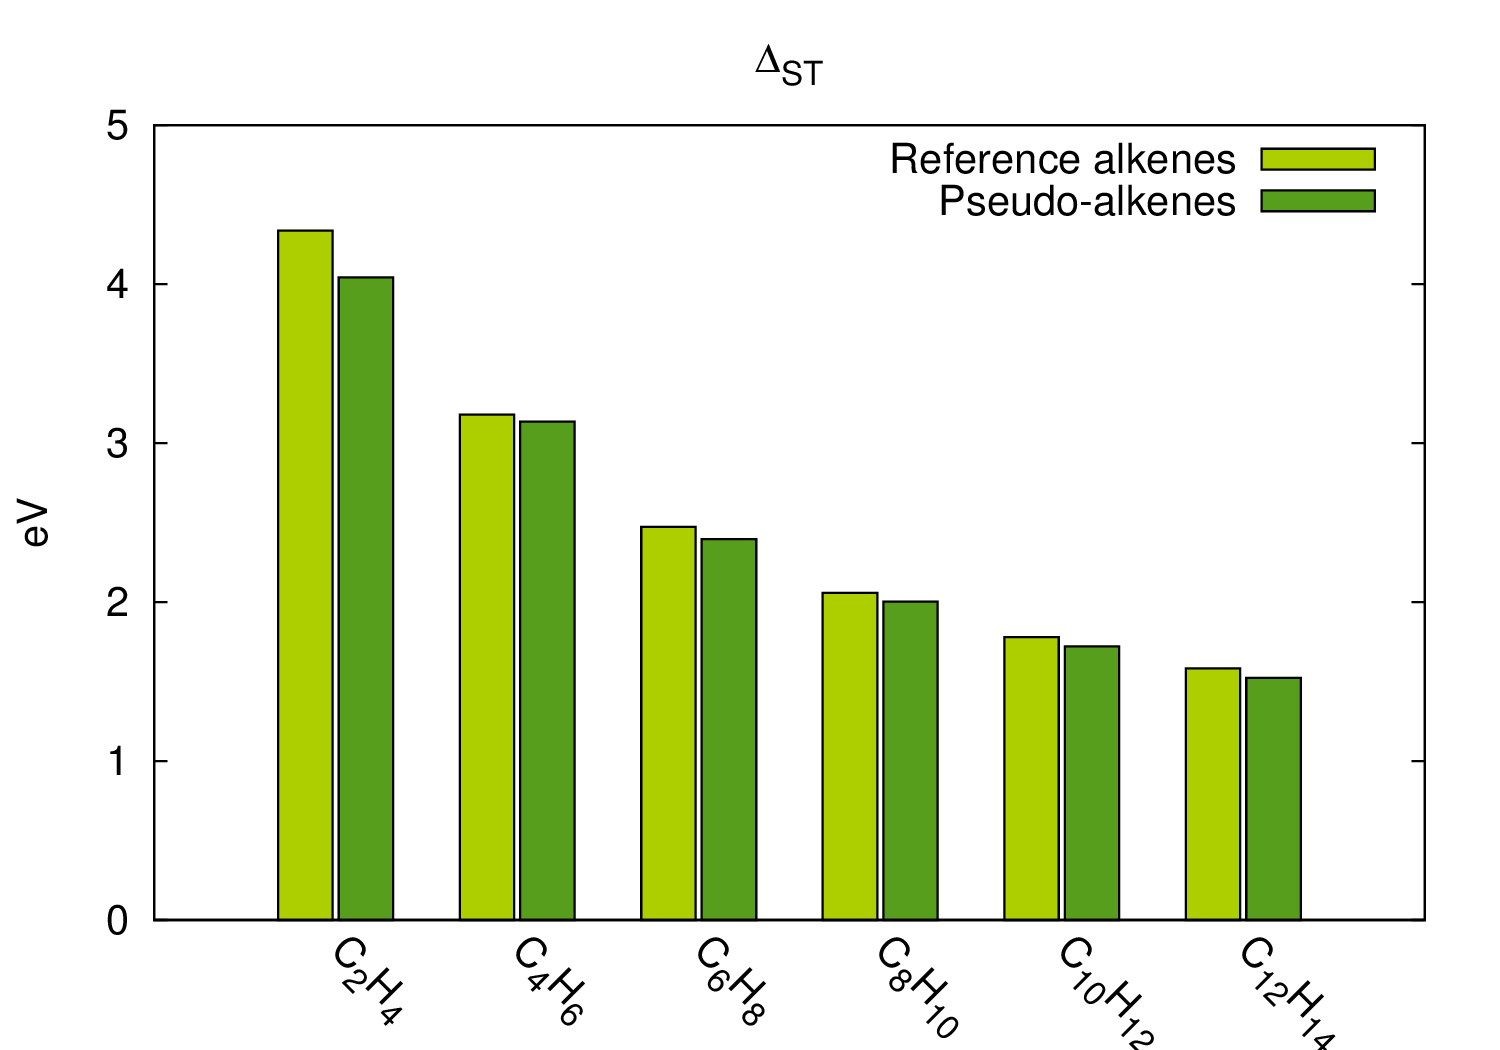
\includegraphics[width=8cm]{short_pbe0_st}
%\caption{DFT (PBE0) comparison of reference and pseudo-system energies across a range of chain alkenes.}
%\label{fig:alkenes_hf_dft}
\end{center}
\vspace{0.25in}
\hspace*{3in}

\caption{DFT (PBE0) comparison of reference and pseudo-system energies across a range of chain alkenes.}
\label{fig:alkenes_hf_dft}
\end{figure}

\begin{figure}
%\vspace*{0.1in}   %%% FIGURE 4
\begin{center}
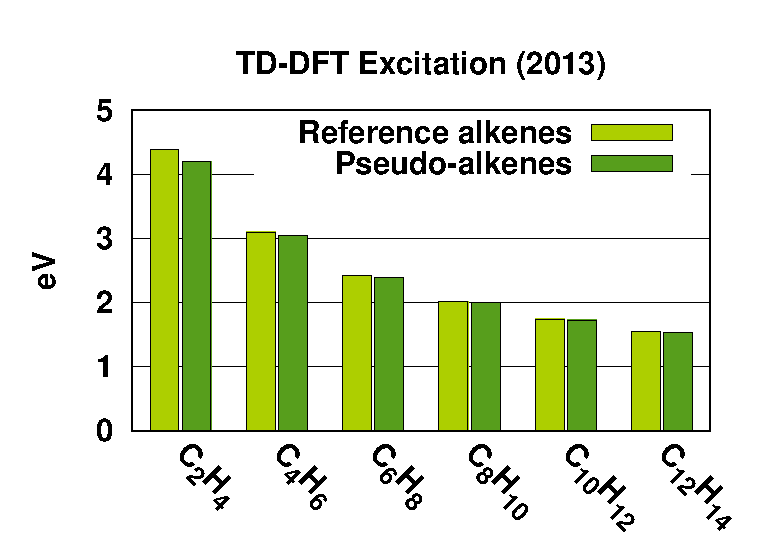
\includegraphics[width=8cm]{short_pbe0_tddft_2013}
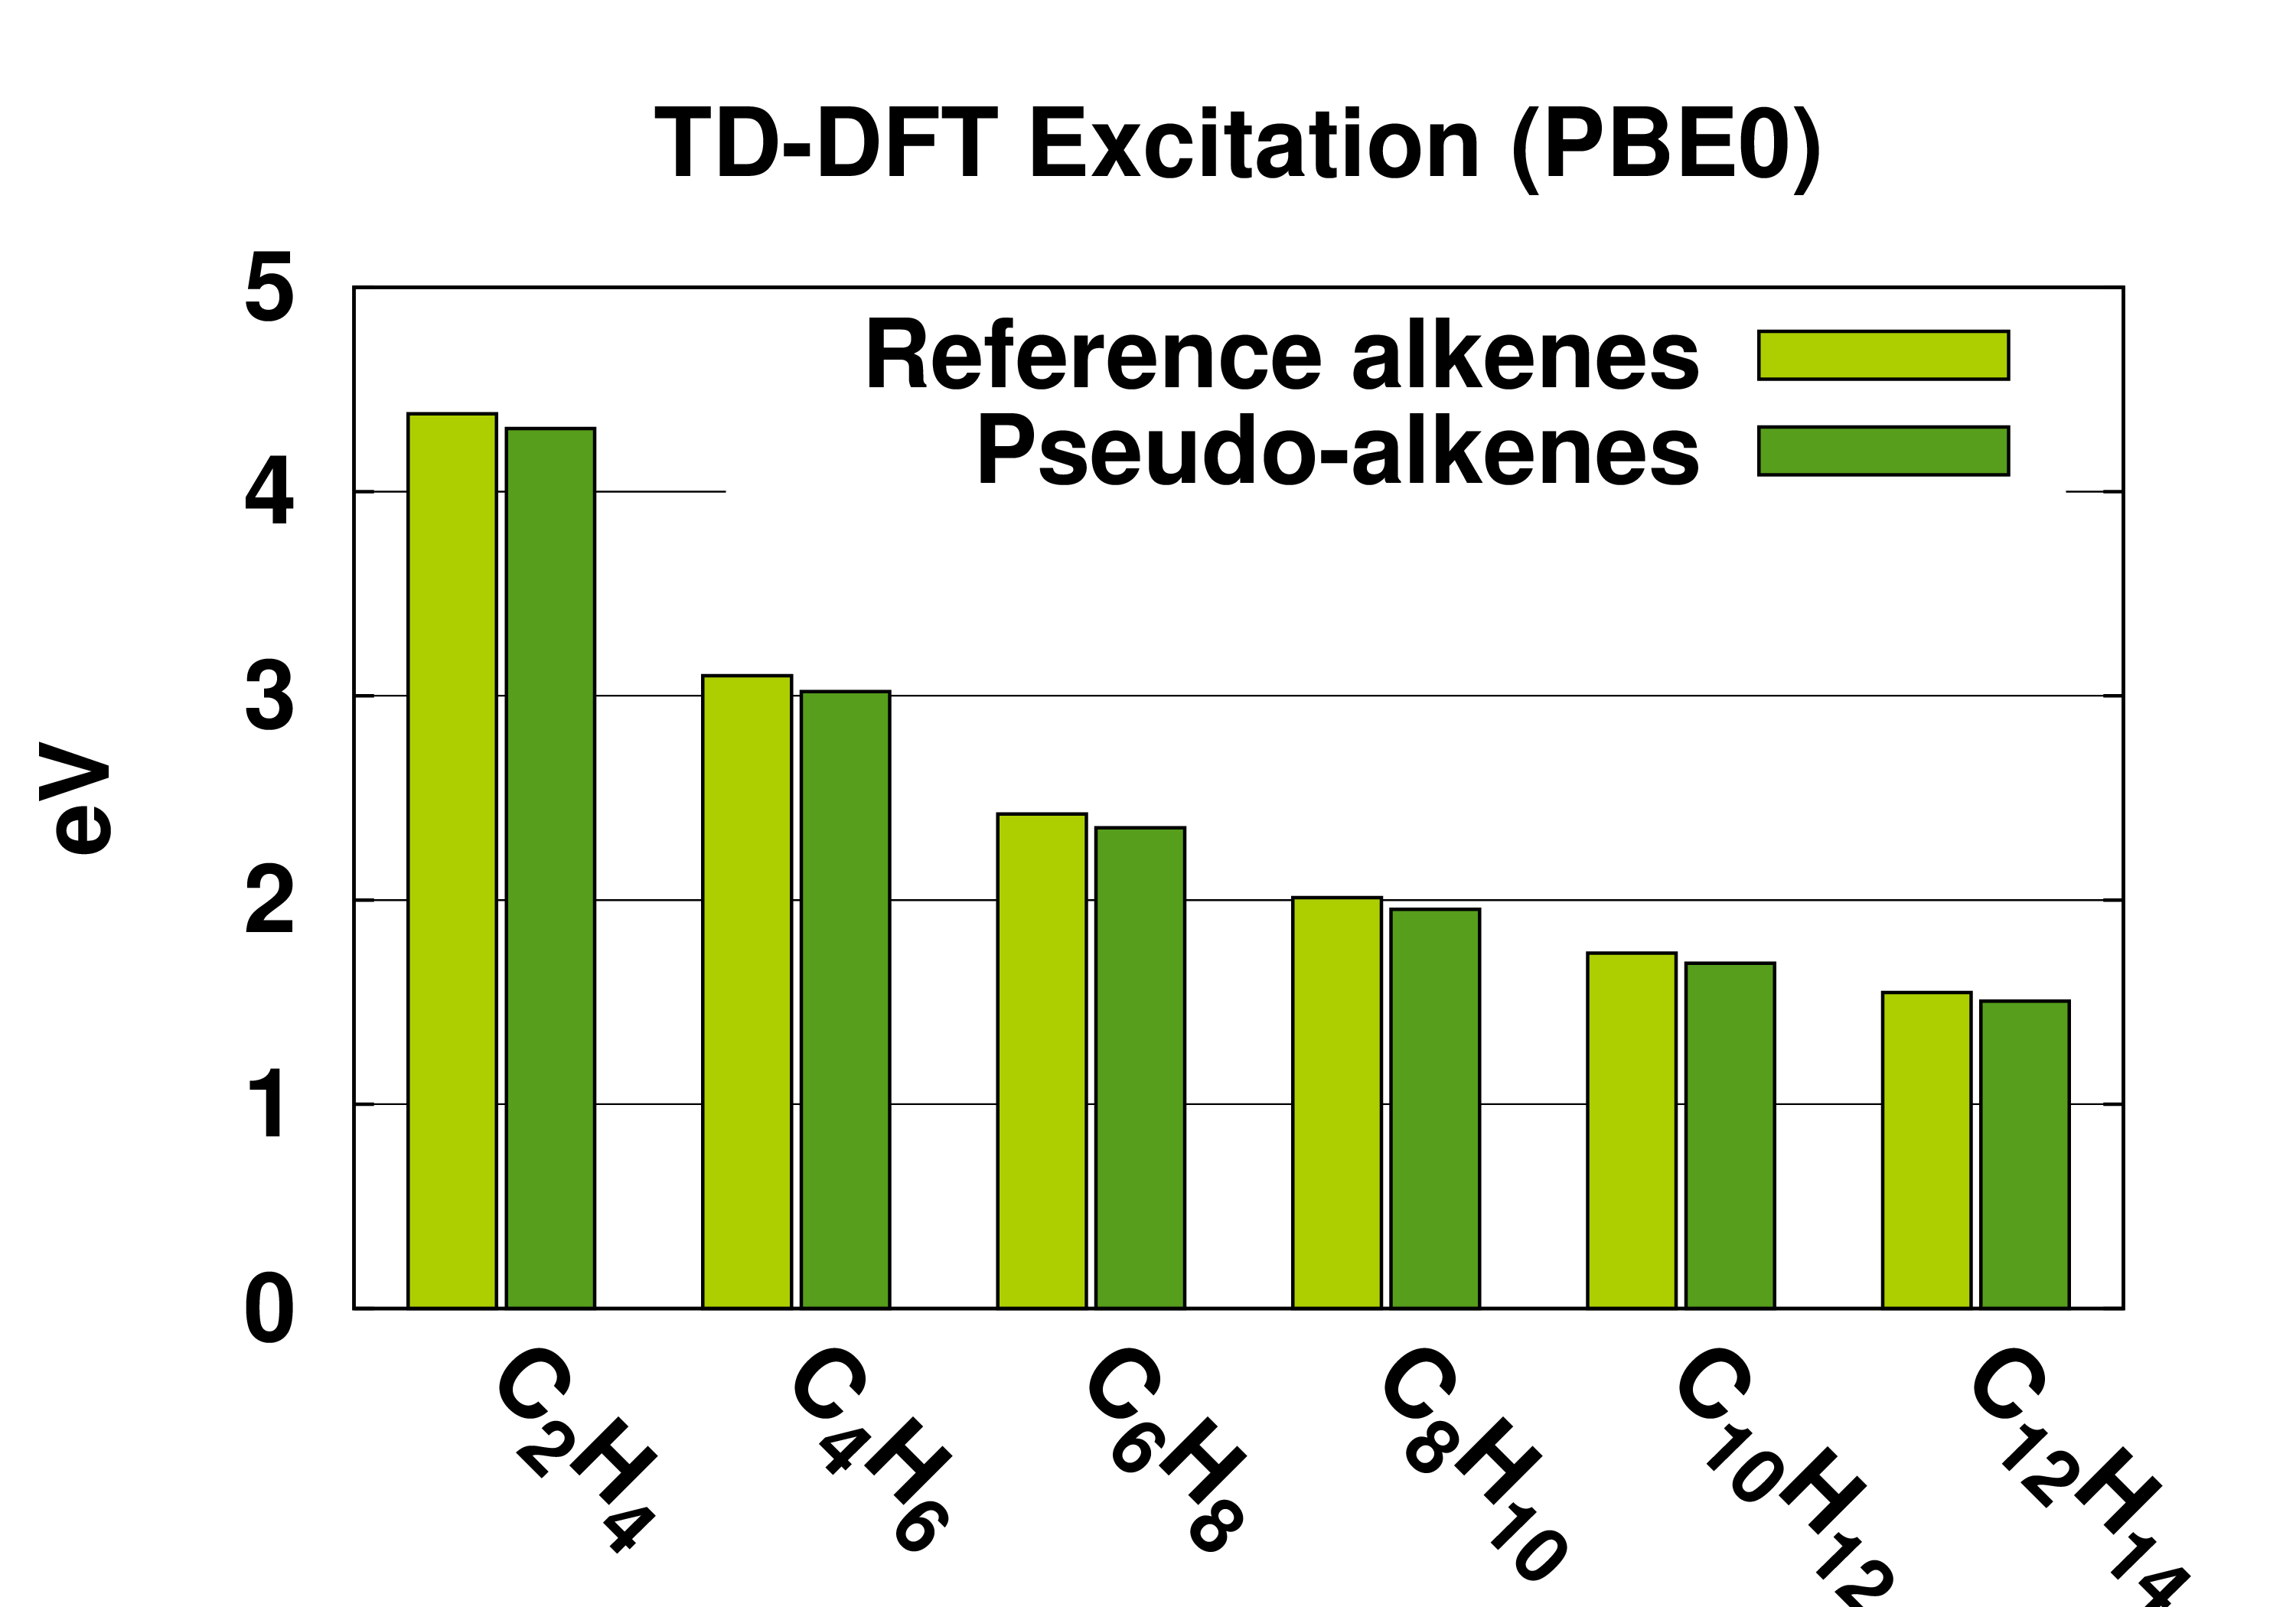
\includegraphics[width=8cm]{short_pbe0_tddft}
%\caption{Comparison of pseudo-alkenes with previous\cite{drujon_pseudopotentials_2013} and current potentials using TD-DFT excitation energies.}
%\label{fig:alkenes_tddft}
\end{center}
\vspace{0.25in}
\hspace*{3in}

\caption{Comparison of pseudo-alkenes with previous\cite{drujon_pseudopotentials_2013} and current potentials using TD-DFT excitation energies.}
\label{fig:alkenes_tddft}
\end{figure}

\begin{figure}
%\vspace*{0.1in}   %%% FIGURE 5
\begin{center}
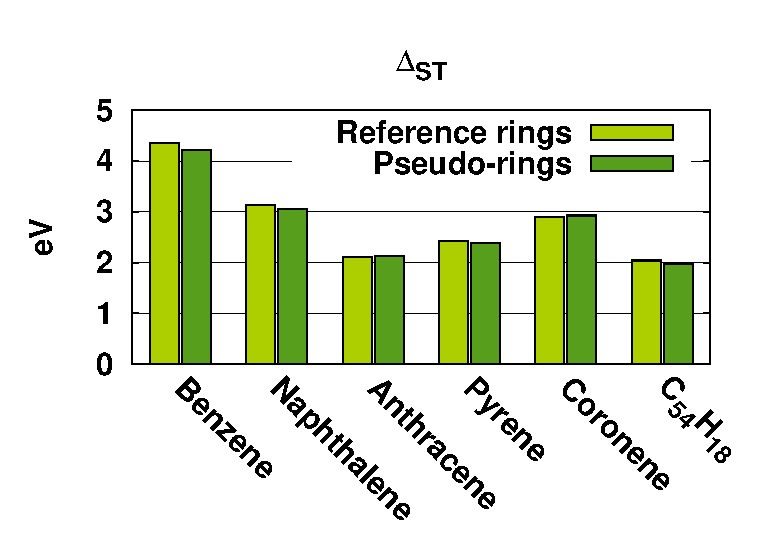
\includegraphics[width=8cm]{ring_pbe0_st}
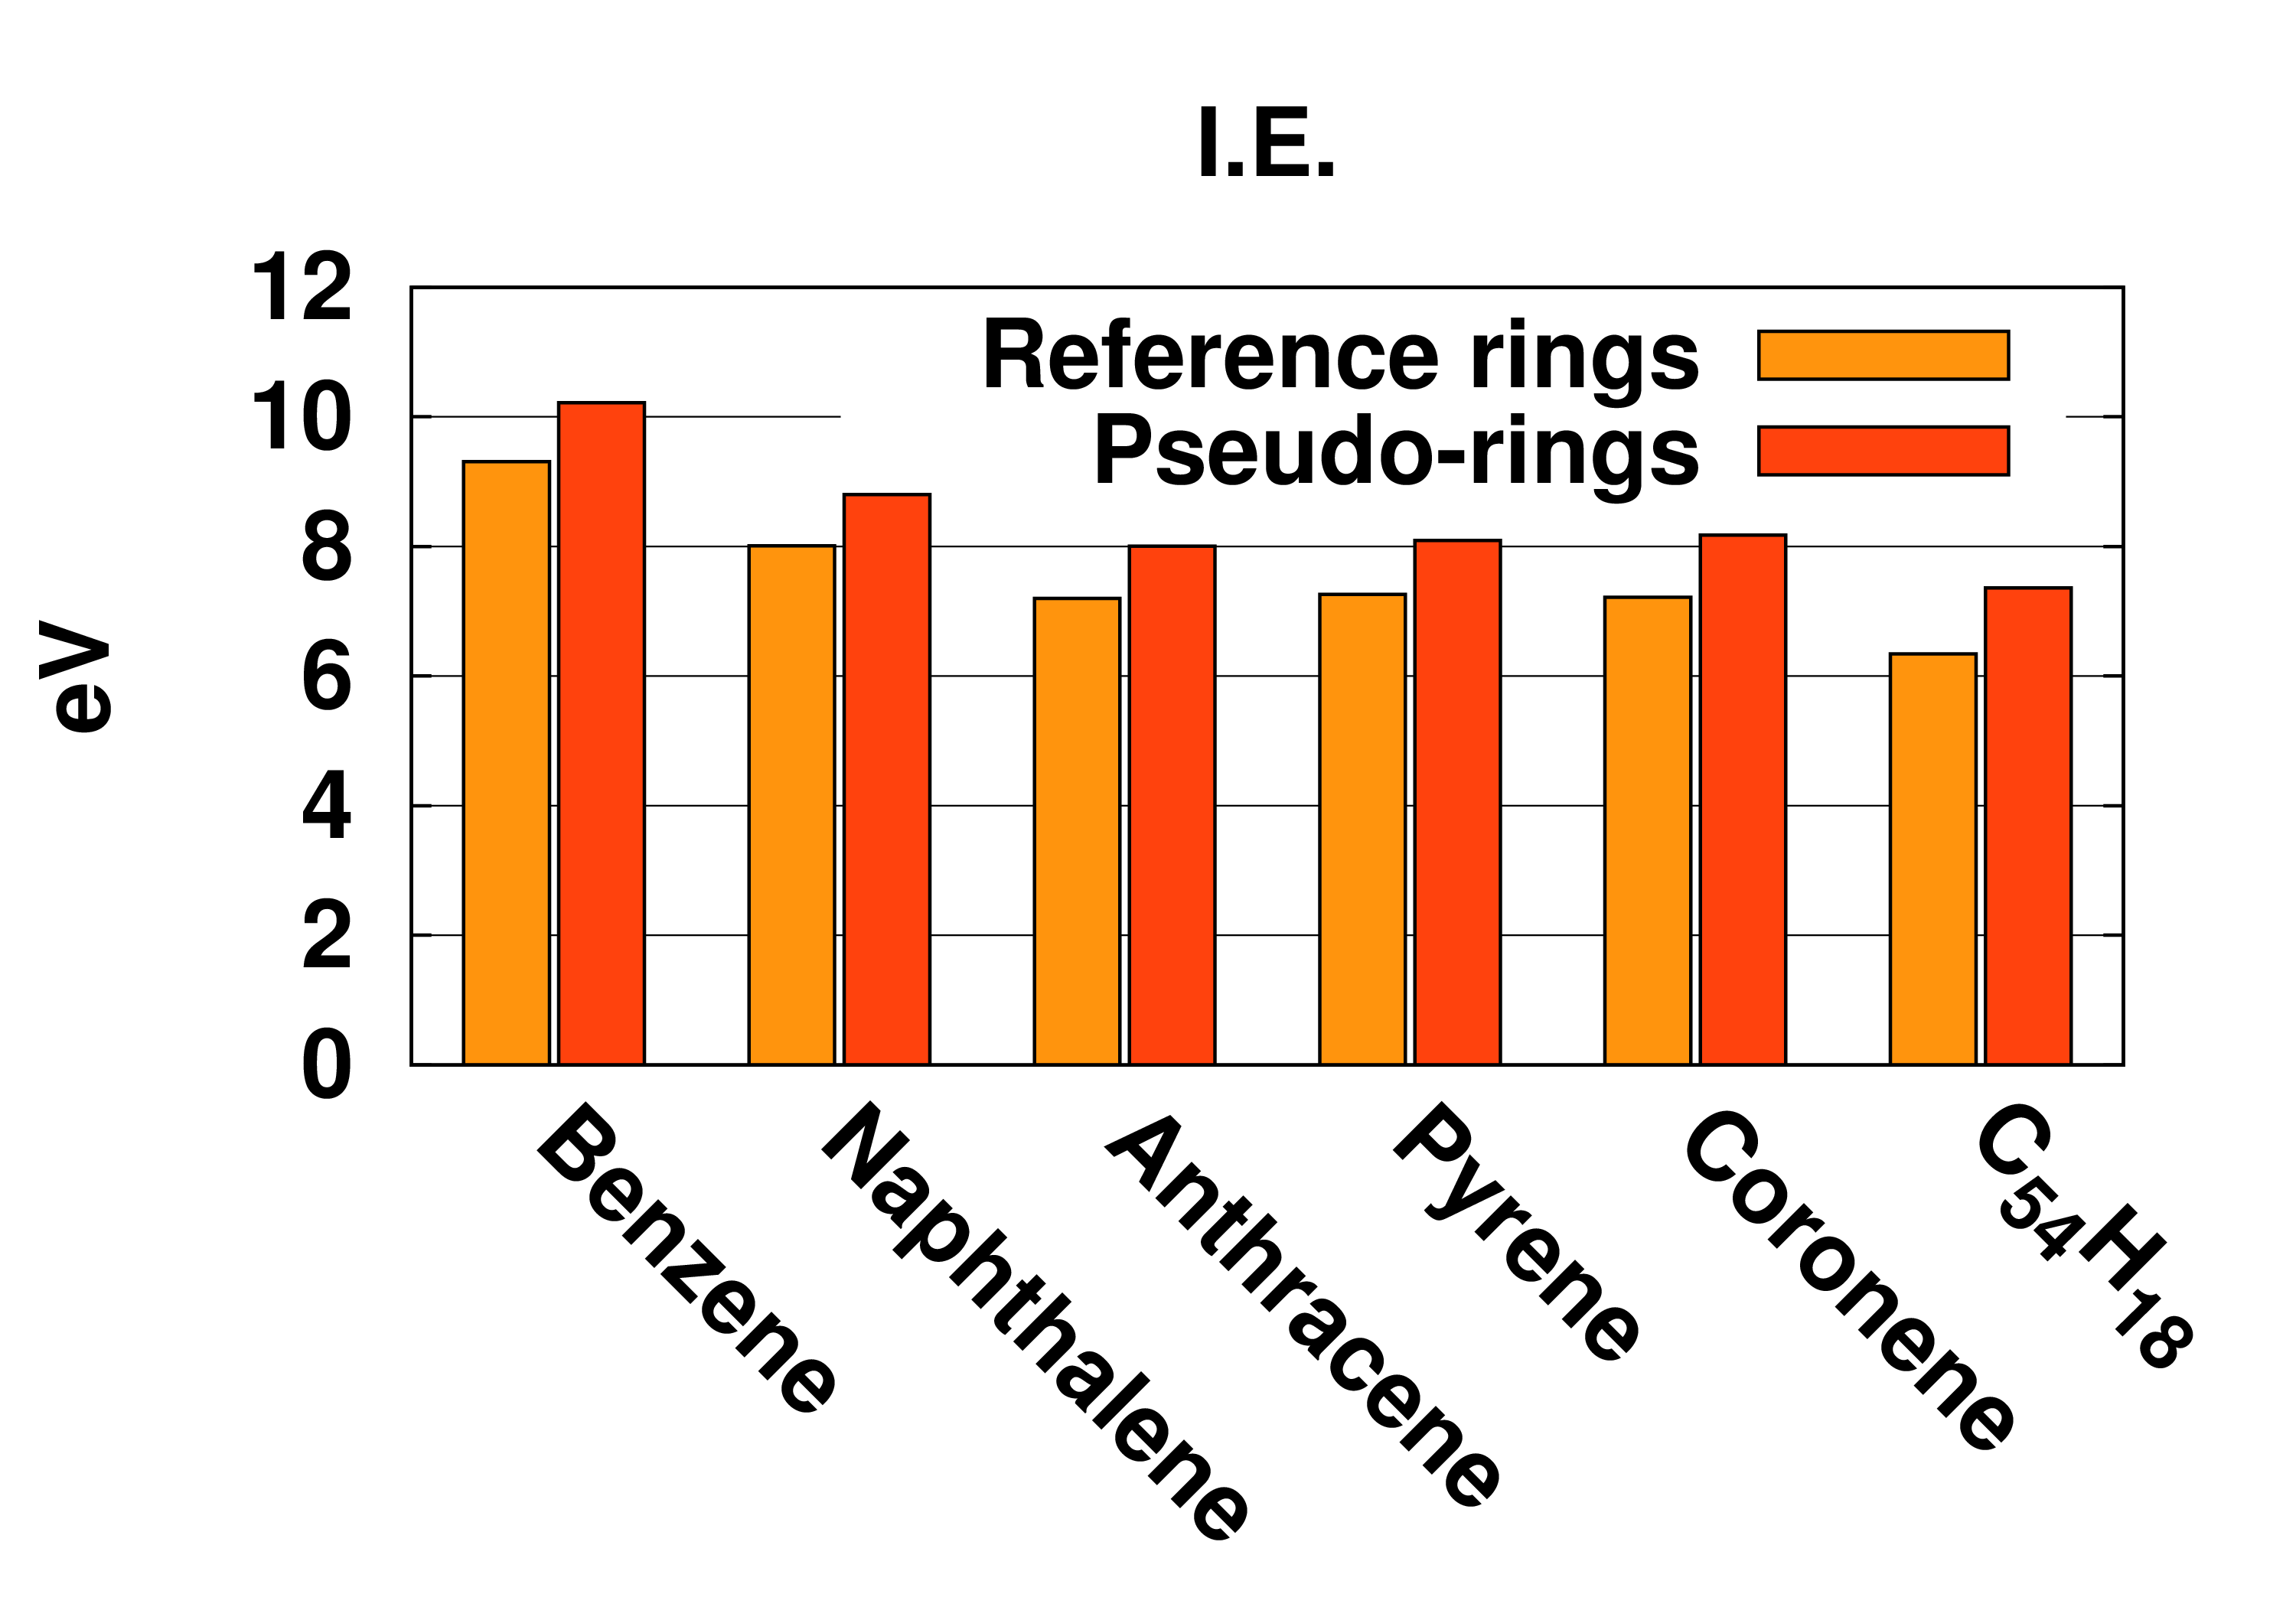
\includegraphics[width=8cm]{ring_pbe0_ie}
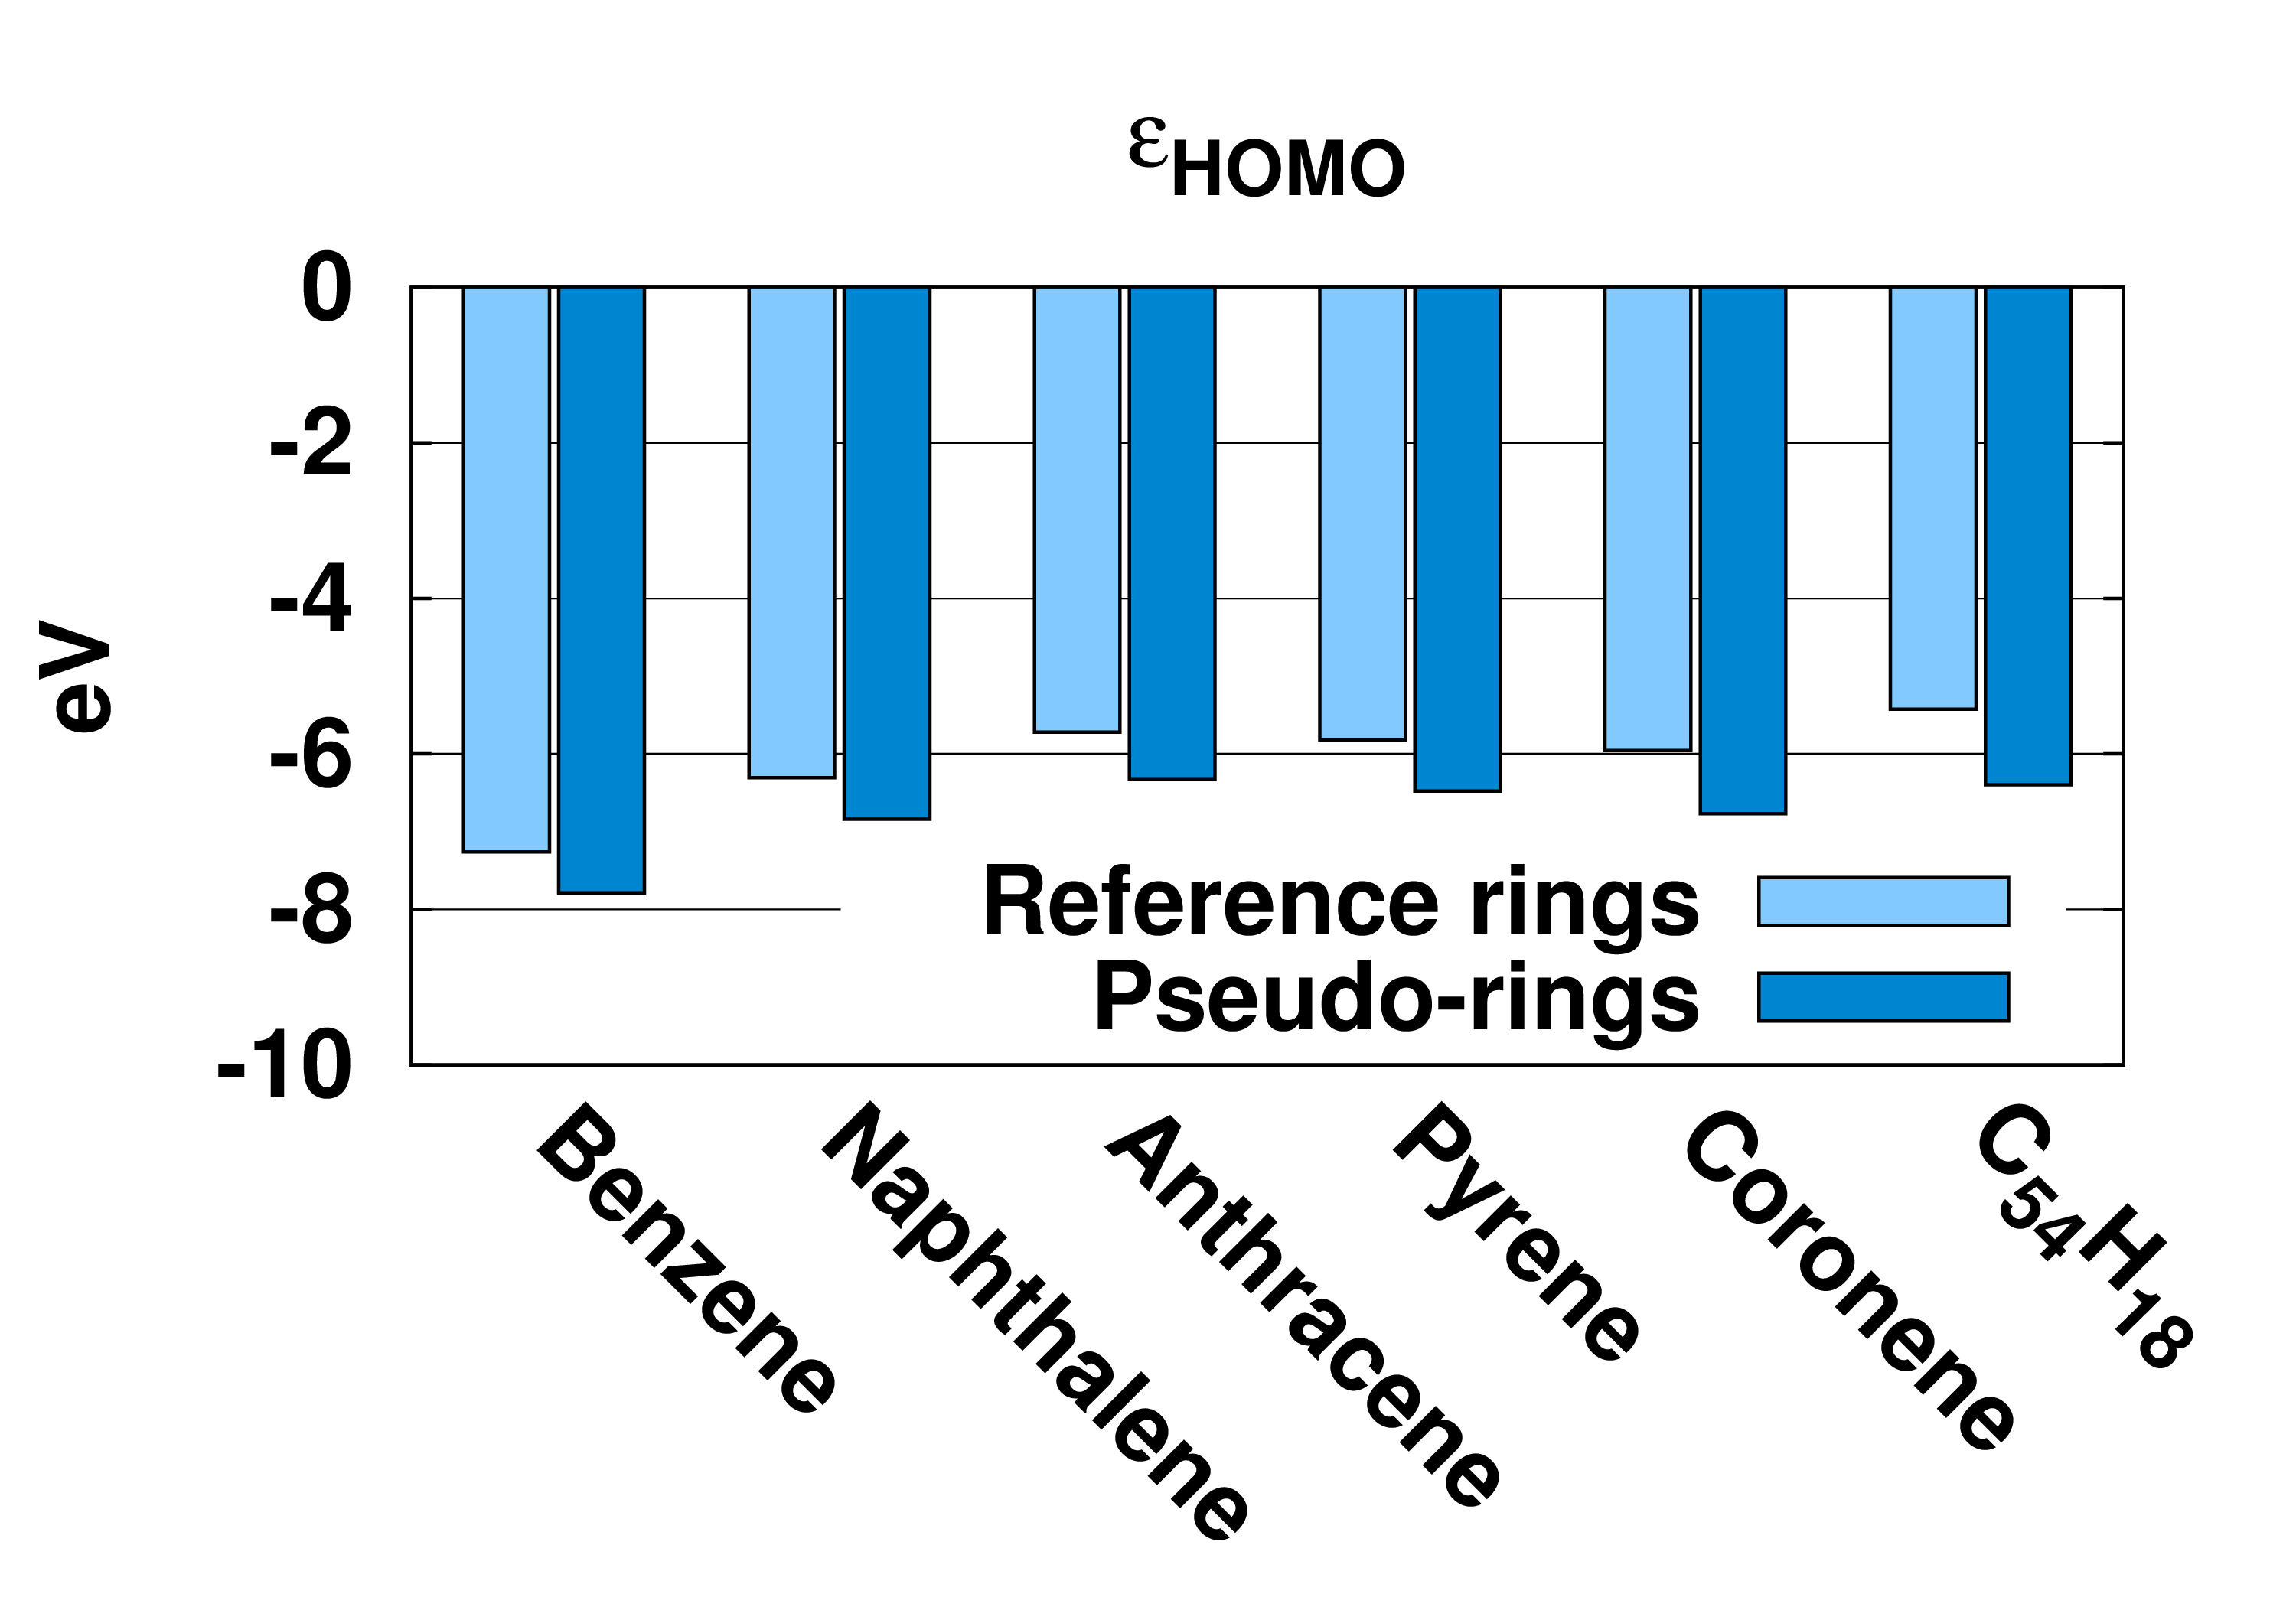
\includegraphics[width=8cm]{ring_pbe0_homo}
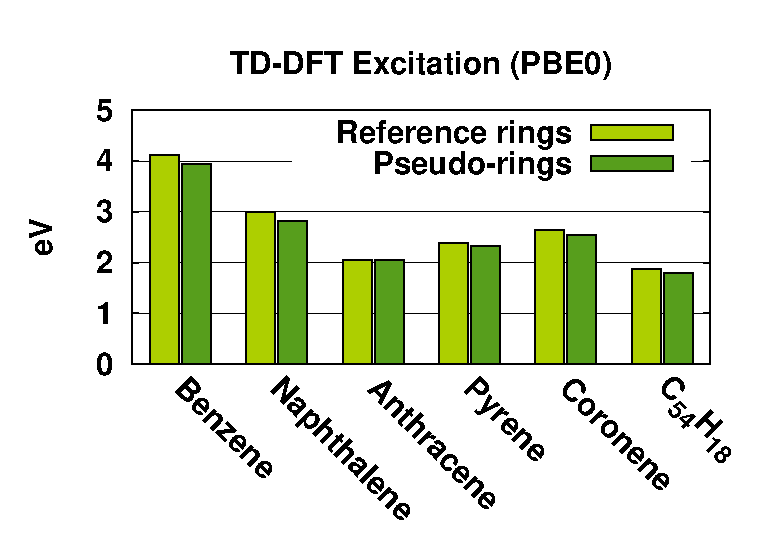
\includegraphics[width=8cm]{ring_pbe0_tddft}
%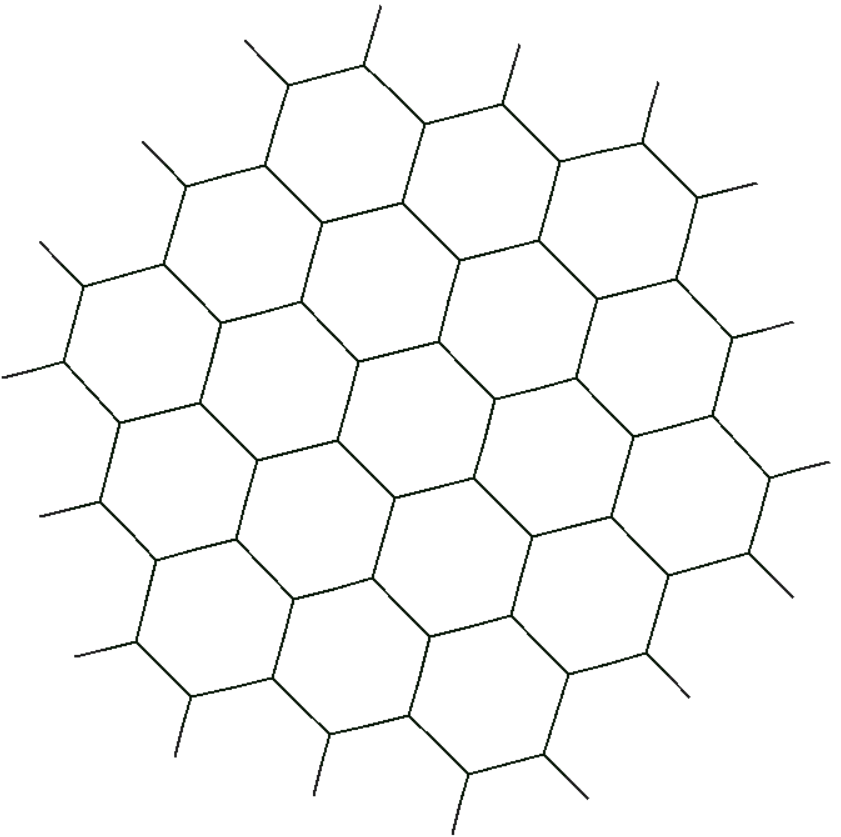
\includegraphics[width=5cm]{19_ring_diagram}
\fbox{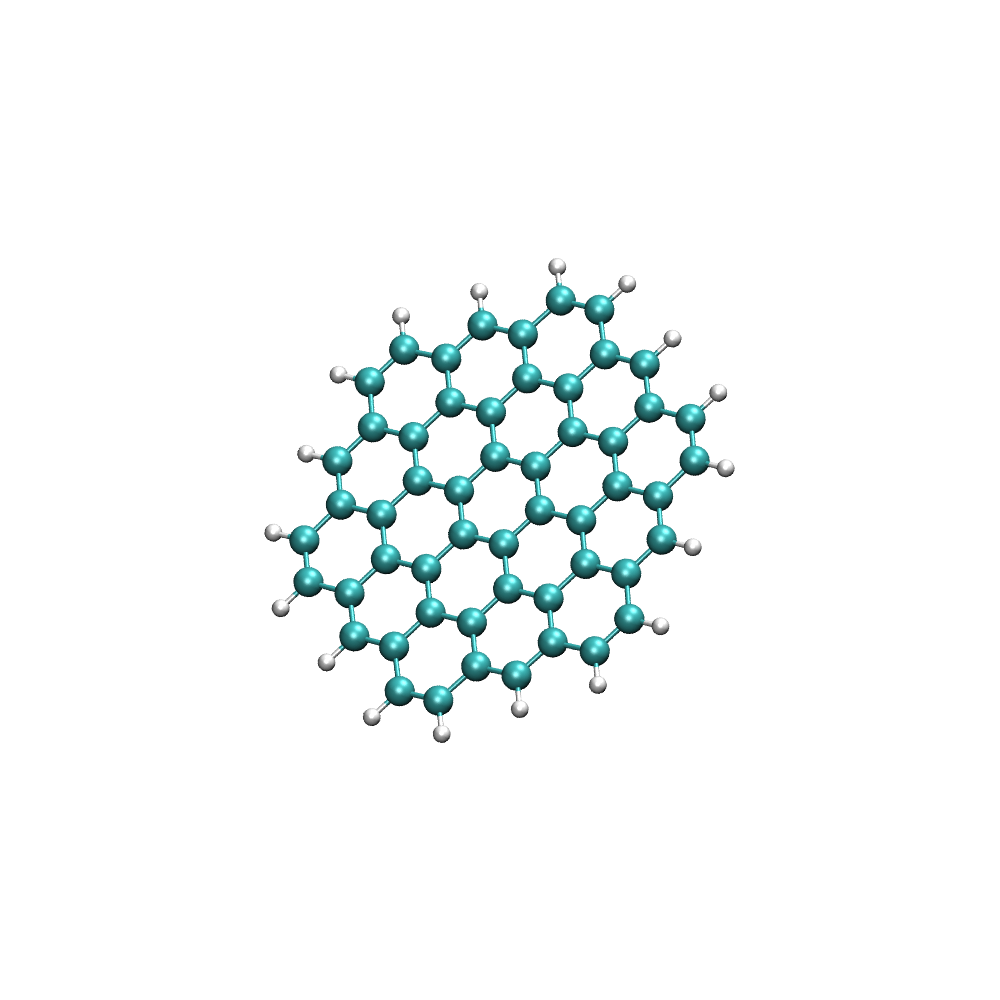
\includegraphics[width=5cm]{c54h18}}
%\caption{DFT and TD-DFT (PBE0) comparison of reference and pseudo-system energies across a range of ring molecules. 
%C\(_{54}\)H\(_{18}\) is shown in the bottom.}
%\label{fig:rings_graphs}
\end{center}
\vspace{0.25in}
\hspace*{3in}

\caption{DFT and TD-DFT (PBE0) comparison of reference and pseudo-system energies across a range of ring molecules. 
C\(_{54}\)H\(_{18}\) is shown in the bottom.}
\label{fig:rings_graphs}
\end{figure}

\begin{figure}
%\vspace*{0.1in}   %%% FIGURE 6
\begin{center}
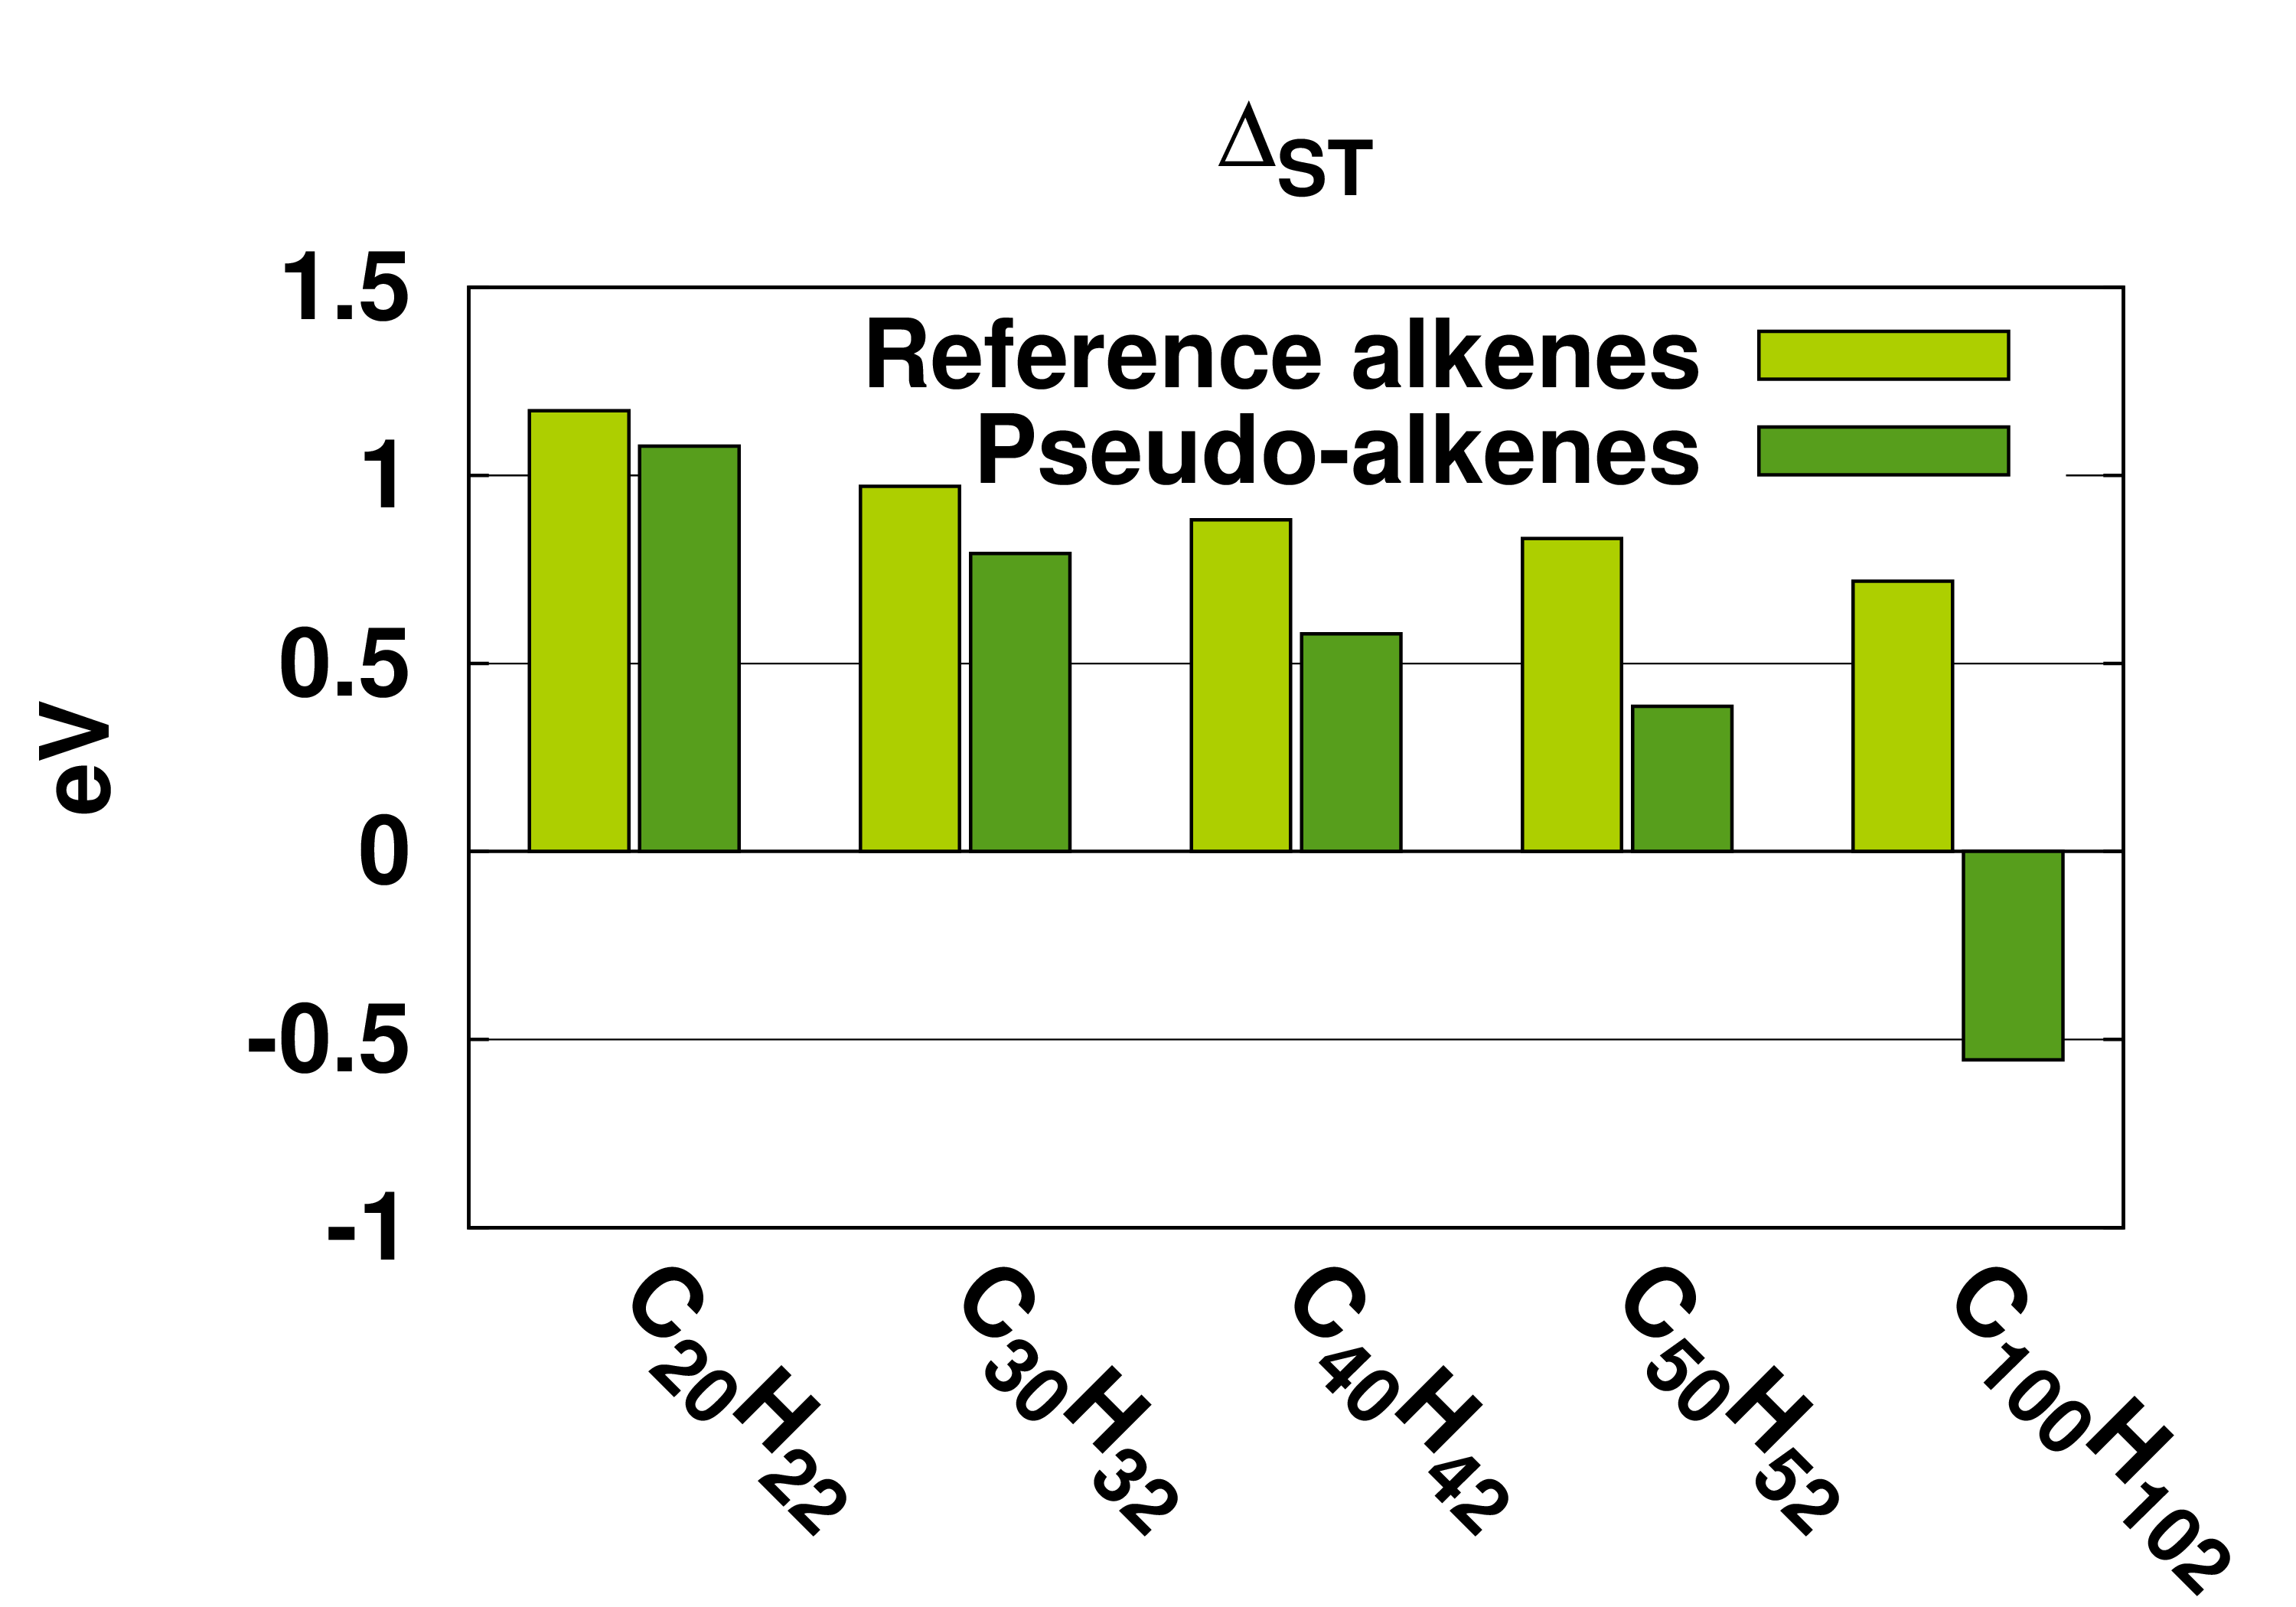
\includegraphics[width=8cm]{long_pbe0_st}
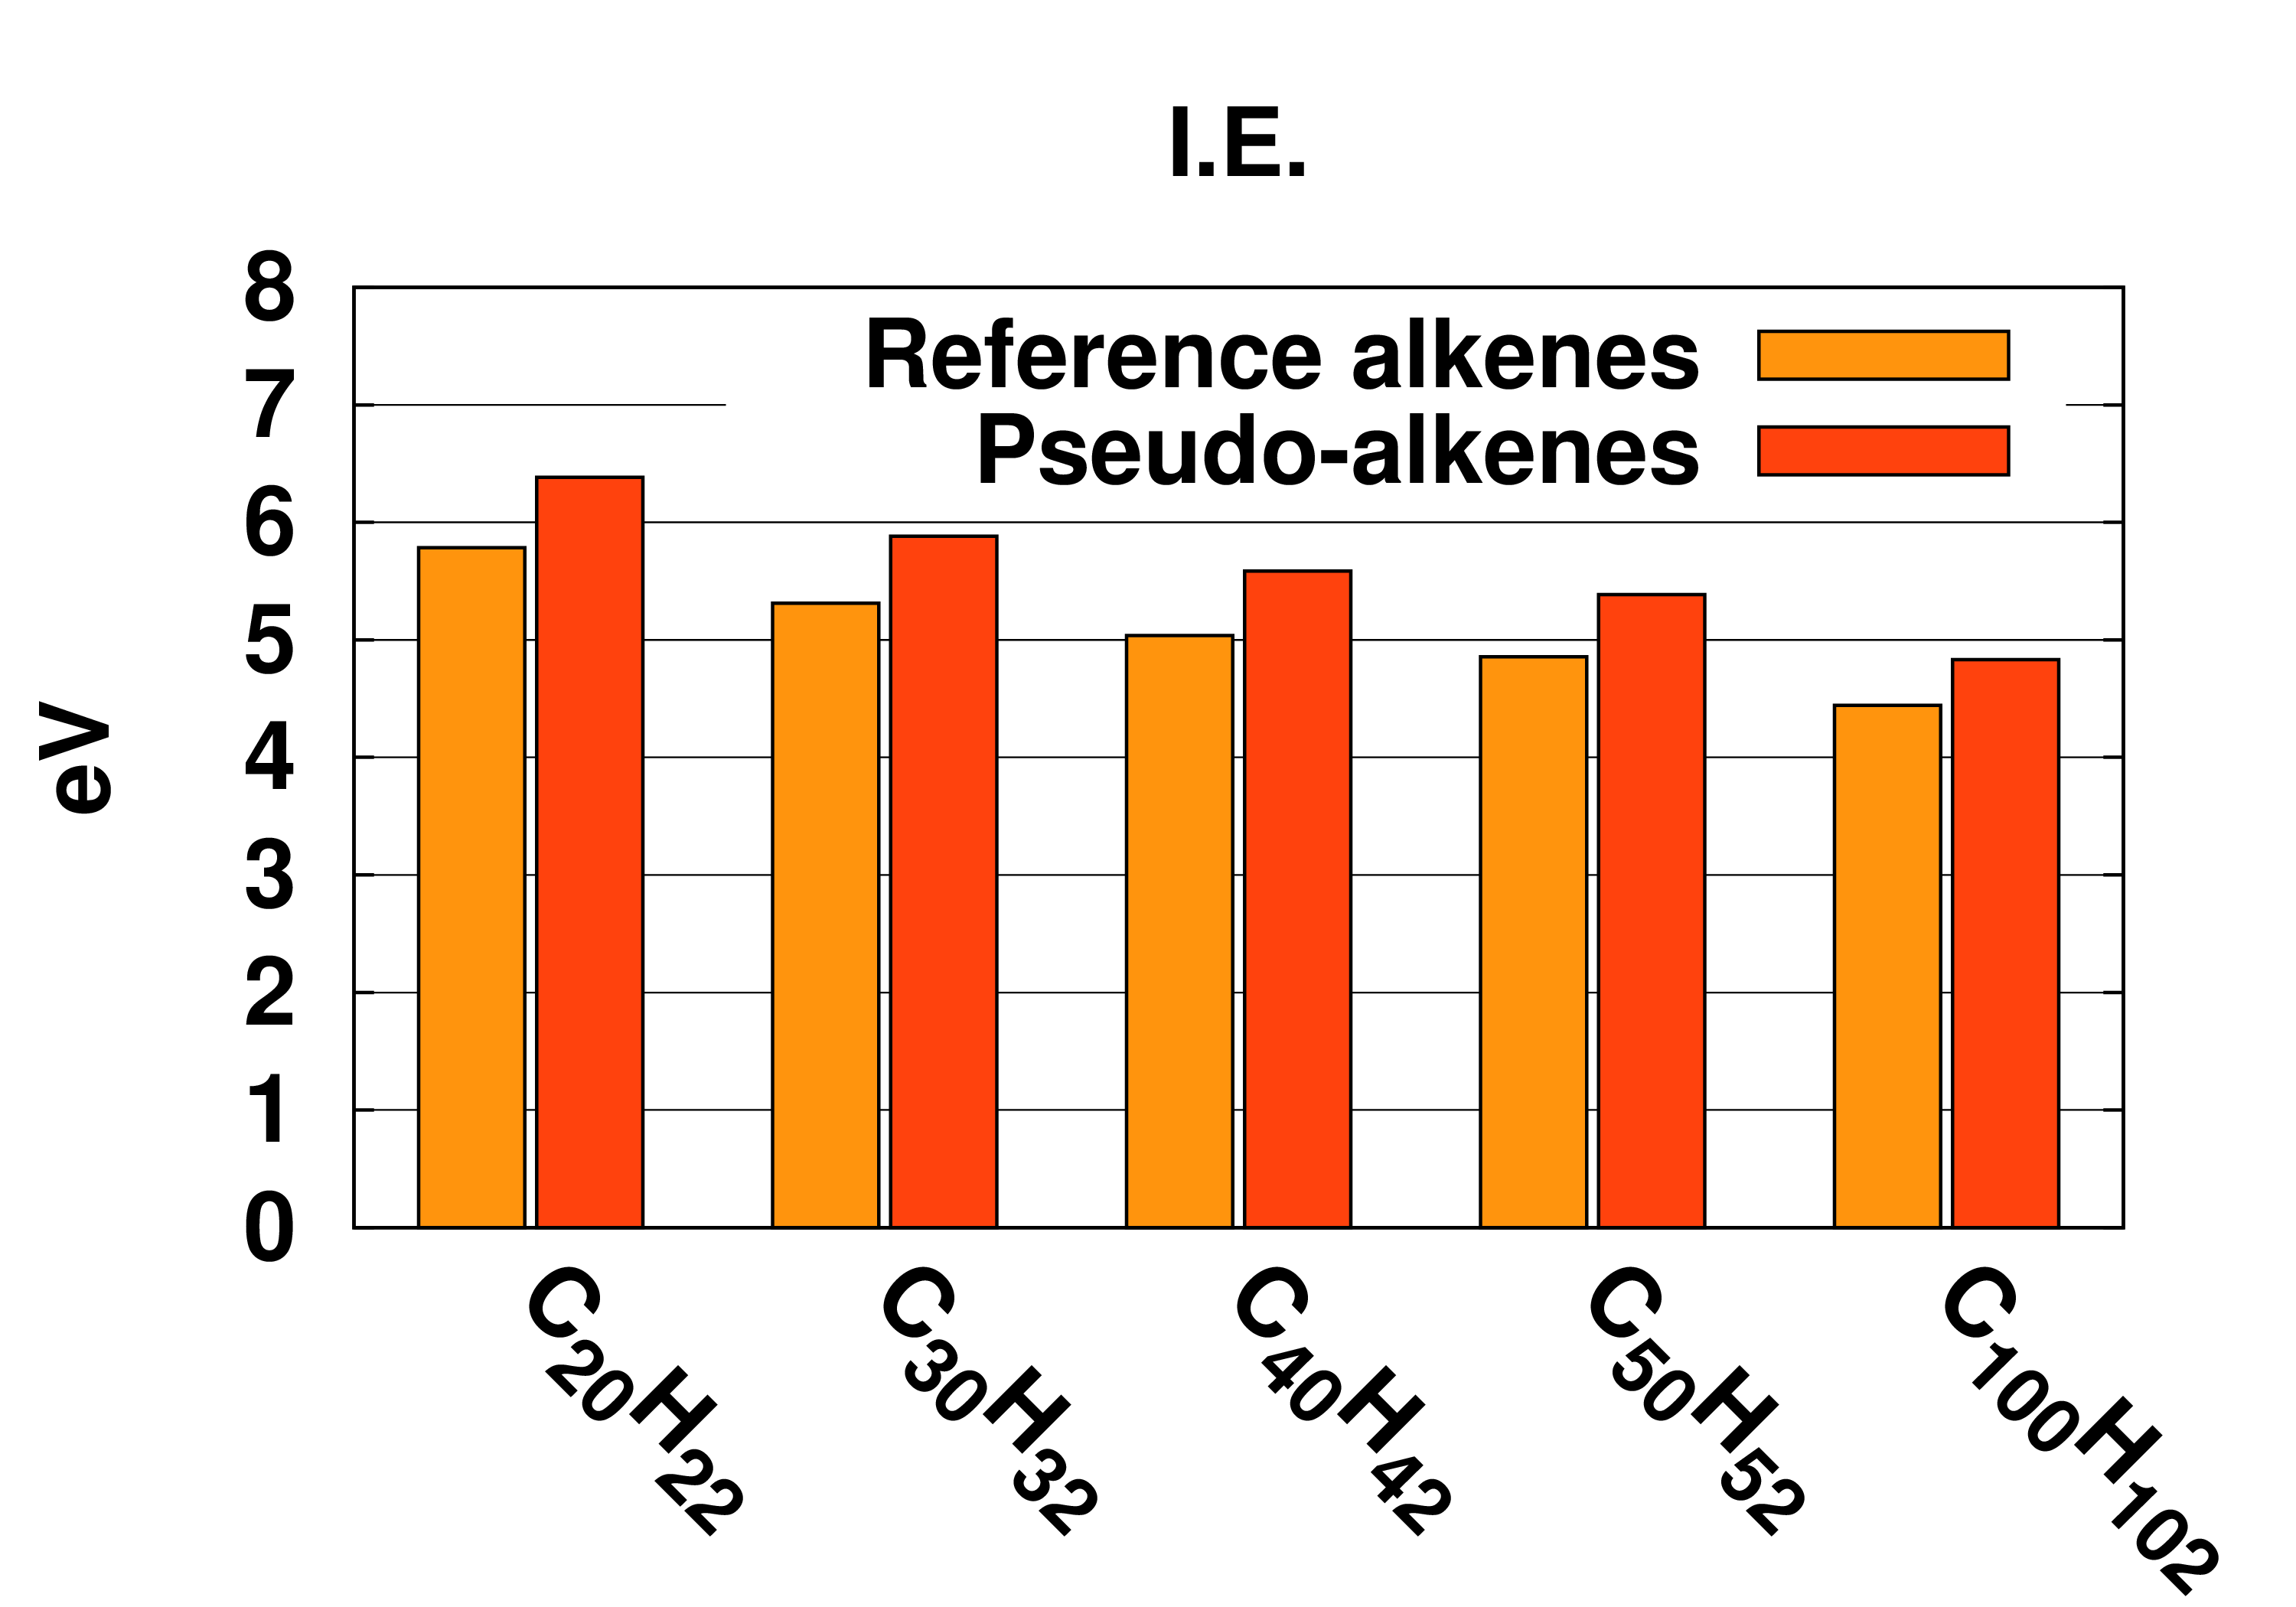
\includegraphics[width=8cm]{long_pbe0_ie}
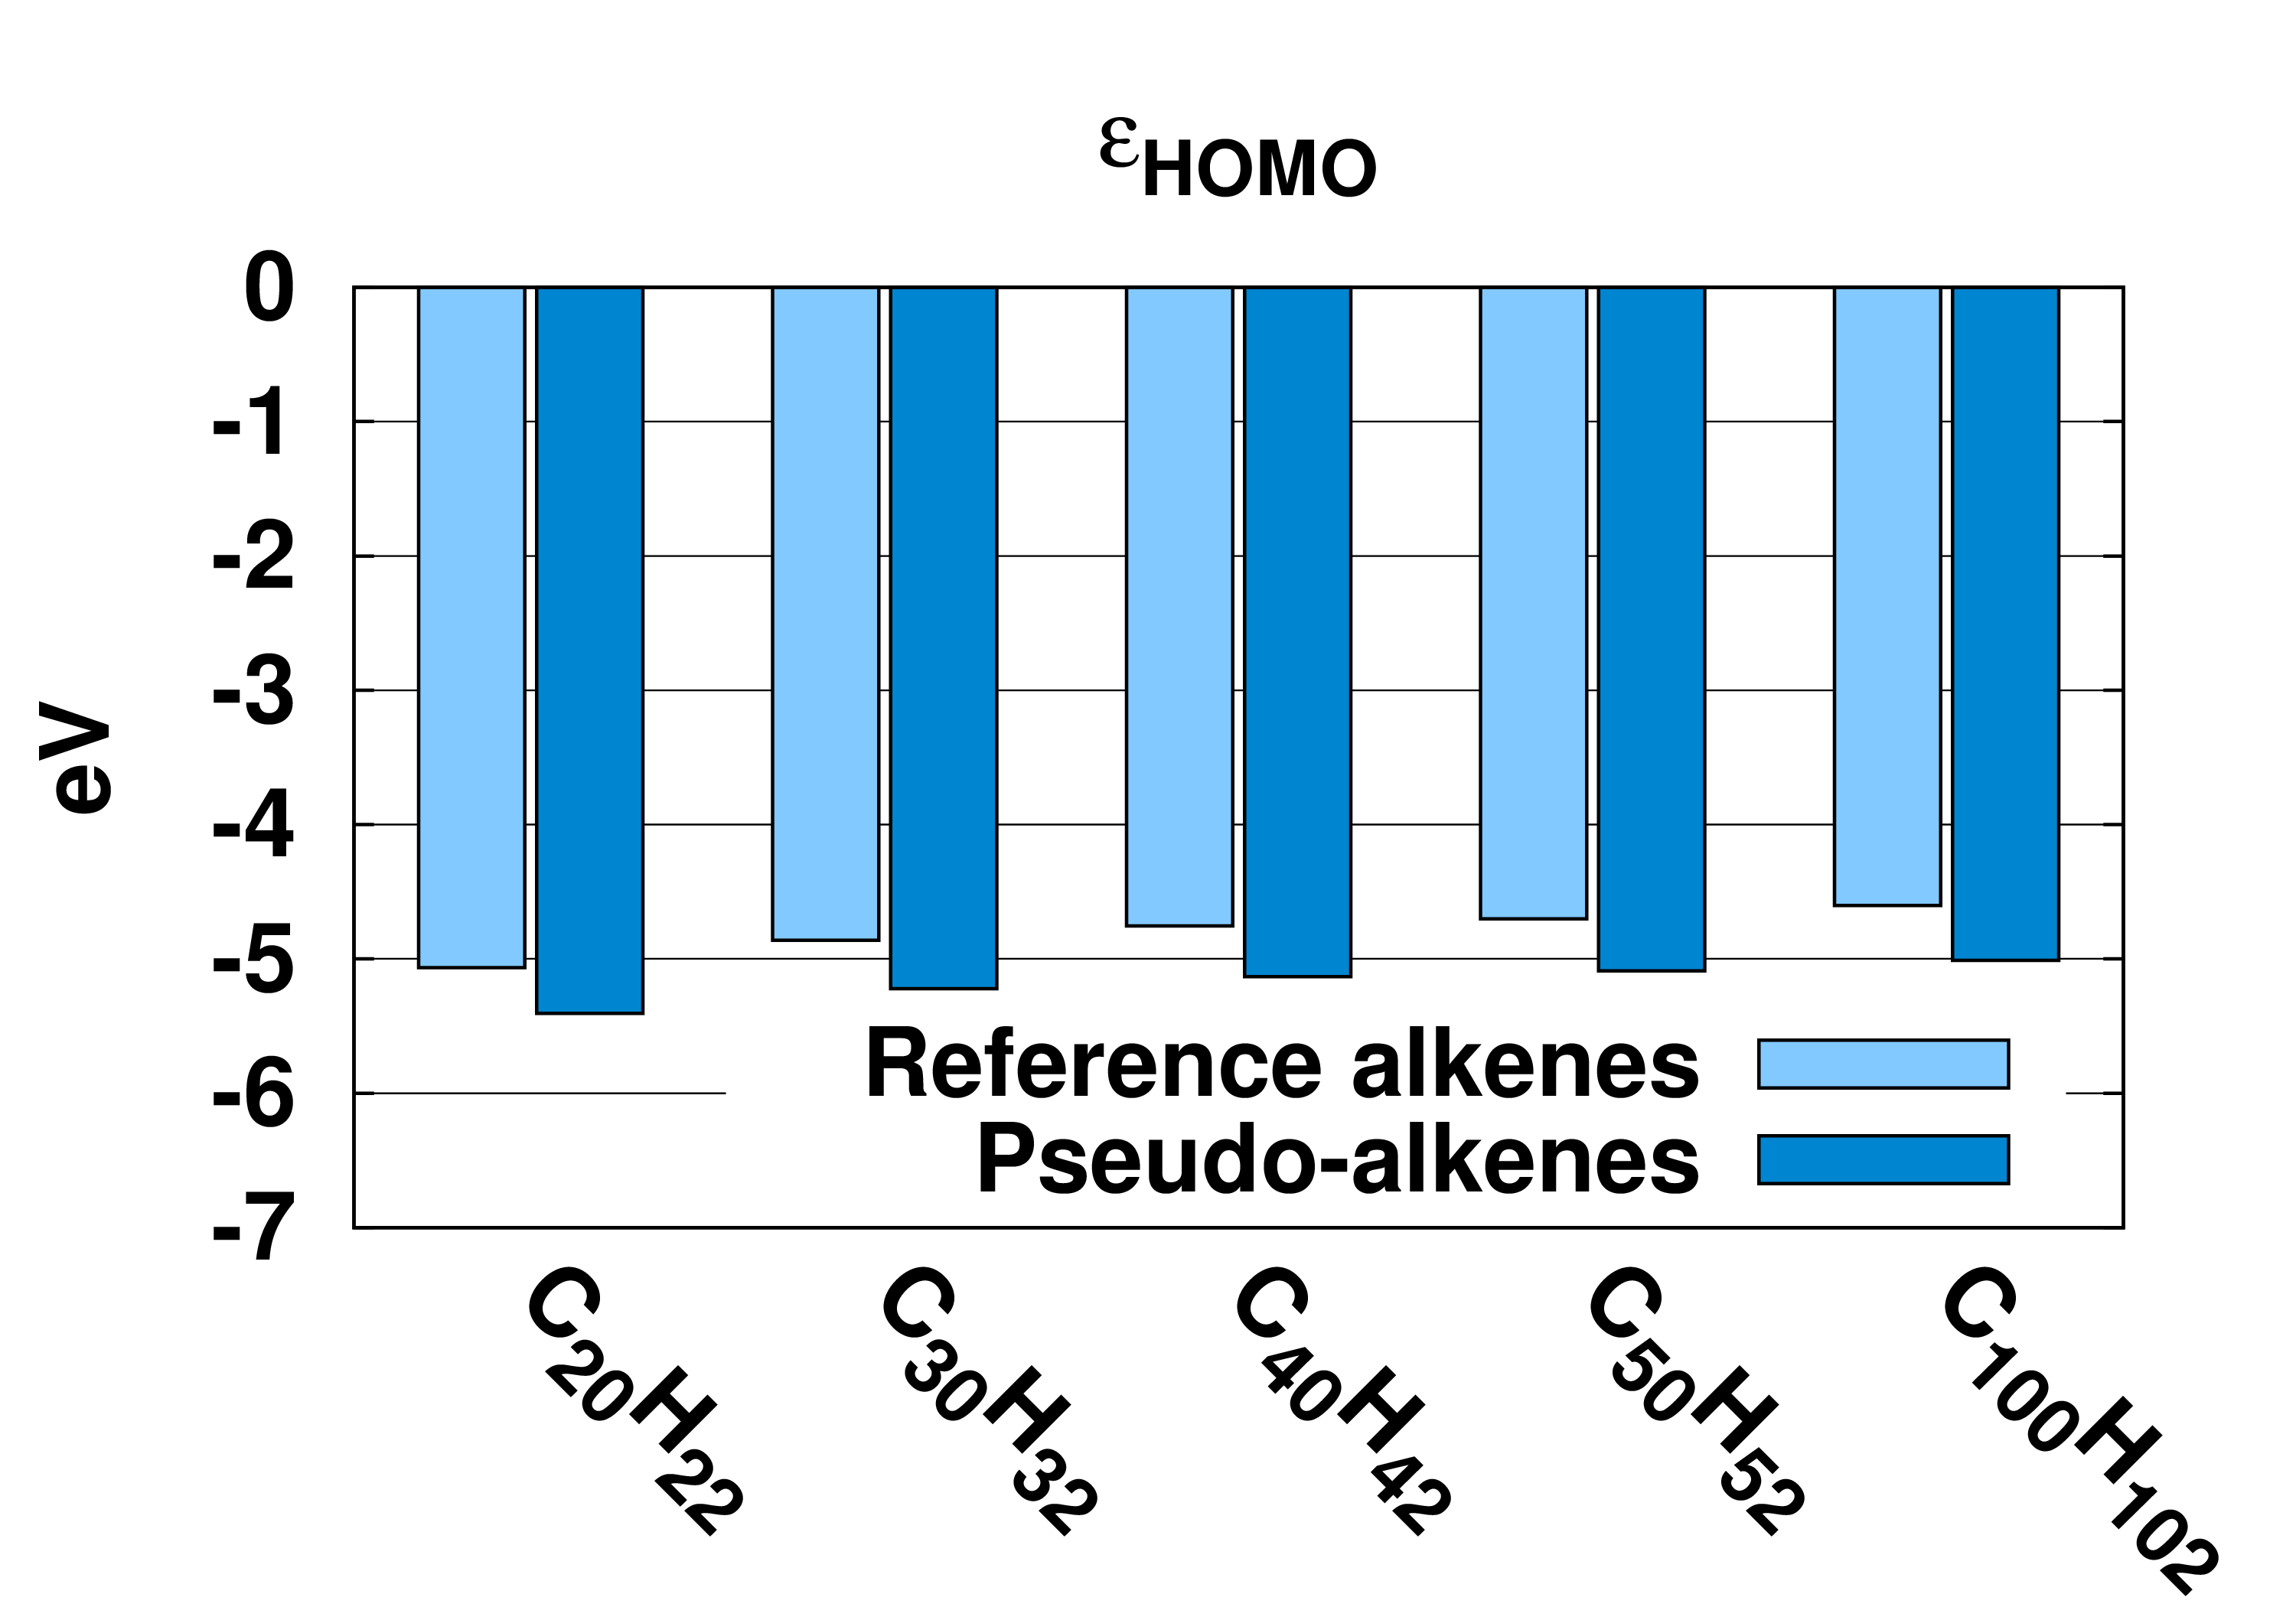
\includegraphics[width=8cm]{long_pbe0_homo}
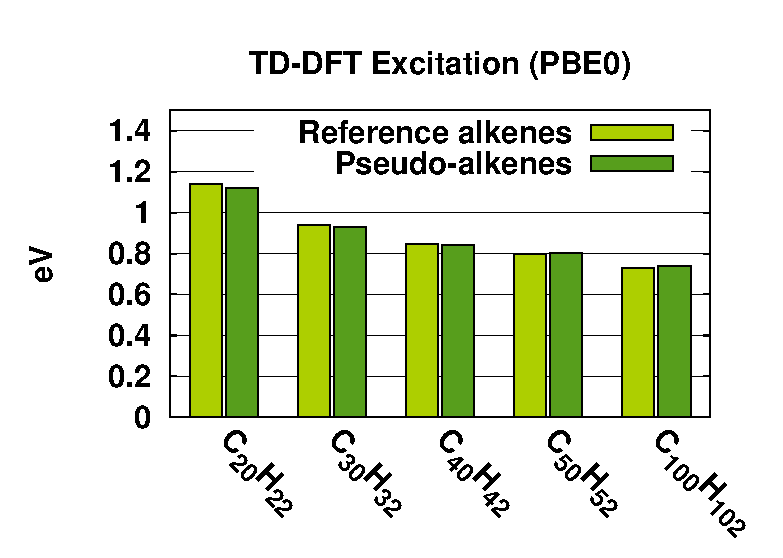
\includegraphics[width=8cm]{long_pbe0_tddft}
%\caption{DFT and TD-DFT (PBE0) comparison of reference and pseudo-system energies across a range of long chain alkenes (C\(_{20}\)-C\(_{100}\)).}
%\label{fig:long_chain_graphs}
\end{center}
\vspace{0.25in}
\hspace*{3in}

\caption{DFT and TD-DFT (PBE0) comparison of reference and pseudo-system energies across a range of long chain alkenes (C\(_{20}\)-C\(_{100}\)).}
\label{fig:long_chain_graphs}
\end{figure}

\begin{figure}
%\vspace*{0.1in}   %%% FIGURE 7
\begin{center}
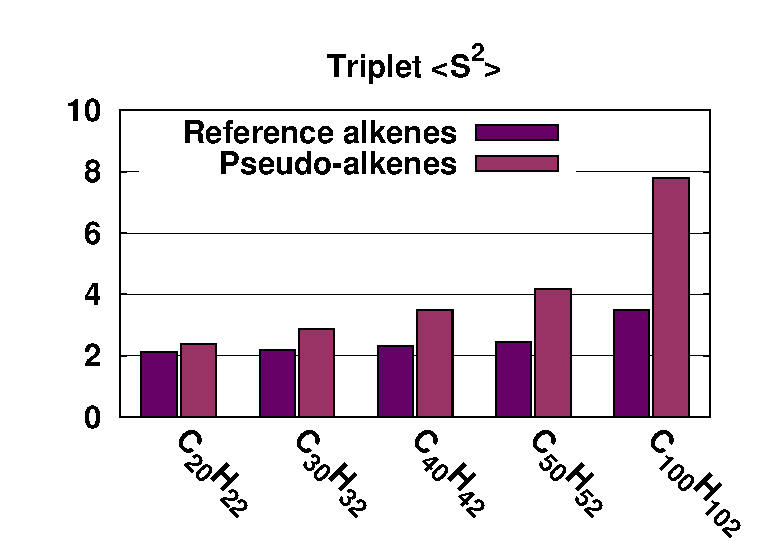
\includegraphics[width=8cm]{long_pbe0_s2}
%\caption{Comparison of $S^2$ expectation values obtained for the calculation
%of the first triplet configuration in a SCF formalism, for reference
%and pseudo-systems.}
%\label{fig:ssquare}
\end{center}
\vspace{0.25in}
\hspace*{3in}
\caption{Comparison of $S^2$ expectation values obtained for the calculation
of the first triplet configuration in a SCF formalism, for reference
and pseudo-systems.}
\label{fig:ssquare}
\end{figure}

\begin{figure}
%\vspace*{0.1in}   %%% FIGURE 8
\begin{center}
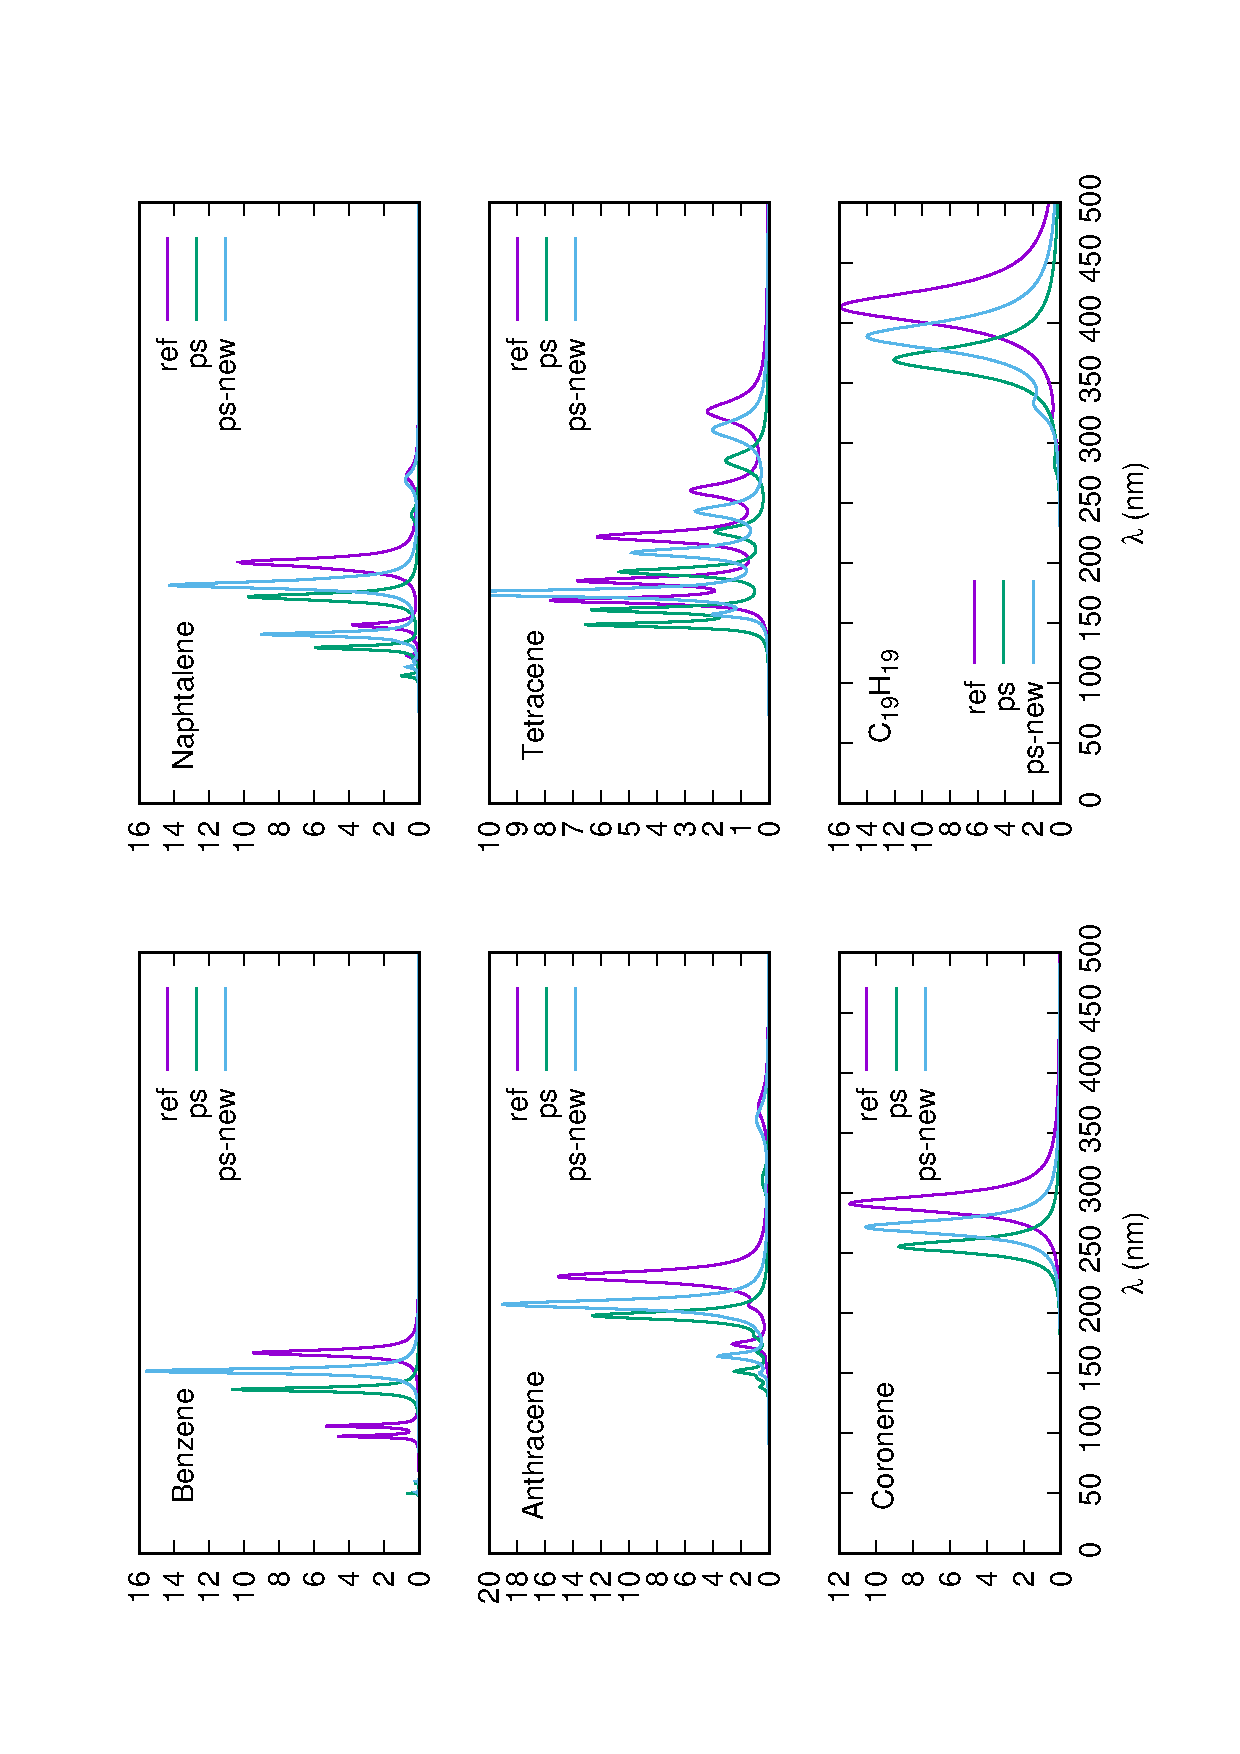
\includegraphics[width=12cm,angle=270]{cnhn_uv}
\end{center}
\vspace{0.25in}
\hspace*{3in}
\caption{Comparison of the UV spectra obtained with pseudo potentials and reference
calculations def2-TZVP/TD-PBE0.}
\label{fig:cnhn_uv}
\end{figure}

%\begin{figure}
%%\vspace*{0.1in}   %%% FIGURE 8
%\begin{center}
%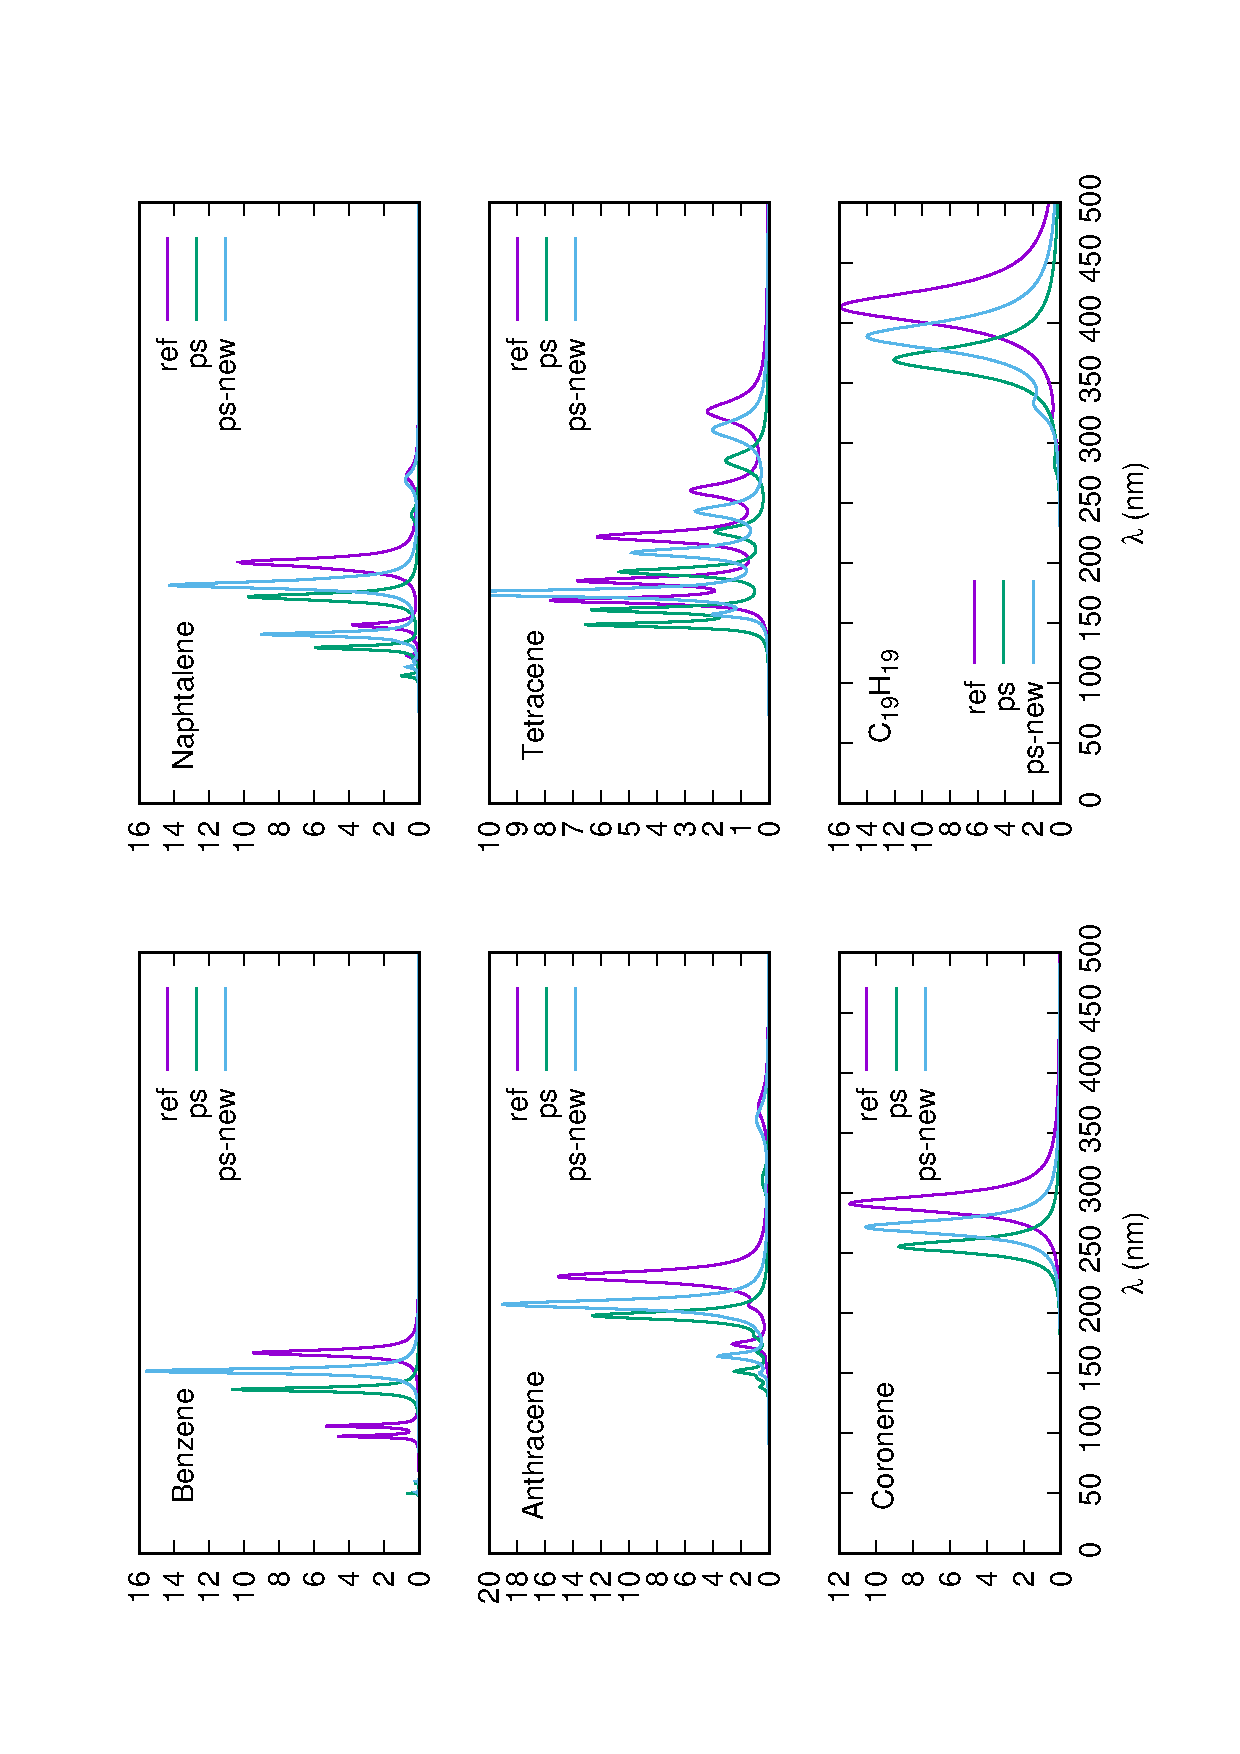
\includegraphics[width=\textwidth]{cnhn_uv}
%\end{center}
%\vspace{0.25in}
%\hspace*{3in}
%\caption{Comparison of the UV spectra obtained with pseudo potentials from the previous section (green), the current section (blue) and reference calculations def2-TZVP/TD-PBE0 (red).}
%\label{fig:cnhn_uv}
%\end{figure}
%%%%%%%%%%%%%%%%%%%%%%%%%%%%

% FIGURES %%%%%%%%%%%%%%%%%%%%%%%%%%%%%%%%%%%%%%%%%%%%%%%%%%%%%%%%%%%%%%%%%%%%%%%%%%%%%%%%%
% FIGURES % FIGURE FILES
% FIGURES 
% FIGURES \clearpage
% FIGURES 
% FIGURES %\vspace*{0.1in}   %%% FIGURE 1
% FIGURES \begin{center}
% FIGURES %\includegraphics[width=0.2\columnwidth,keepaspectratio=true]{cc.eps}
% FIGURES 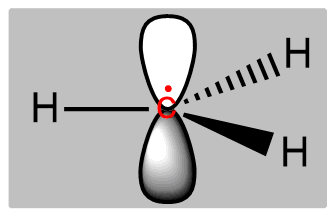
\includegraphics[width=8cm]{ch3.png}
% FIGURES 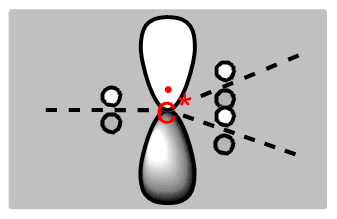
\includegraphics[width=8cm]{pseudoch3.png}
% FIGURES 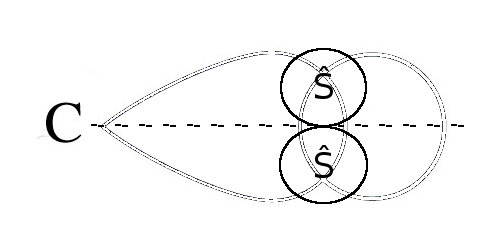
\includegraphics[width=8cm]{tm_sp2_potentials.png}
% FIGURES %\caption{Diagrams of CH\(^{\bullet}_{3}\) (left) and pseudo-CH\(^{\bullet}_{3}\) (right, below) molecules. The pseudo-CH\(^{\bullet}_{3}\) diagrams display the \(s\) and \(p\)-potential positions, and the distances \(d\) and \(c\).}
% FIGURES %\label{figure:ref_pseudo_diagram}
% FIGURES \end{center}
% FIGURES \vspace{0.25in}
% FIGURES \hspace*{3in}
% FIGURES {\Large
% FIGURES \begin{minipage}[t]{3in}
% FIGURES \baselineskip = .5\baselineskip
% FIGURES Figure 1 \\
% FIGURES Alexander Punter, Paola Nava, Yannick Carissan \\
% FIGURES J.\ Comput.\ Chem.
% FIGURES \end{minipage}
% FIGURES }
% FIGURES 
% FIGURES \clearpage
% FIGURES 
% FIGURES %\vspace*{0.1in}   %%% FIGURE 2
% FIGURES \begin{center}
% FIGURES %\includegraphics[width=0.2\columnwidth,keepaspectratio=true]{cc.eps}
% FIGURES \fbox{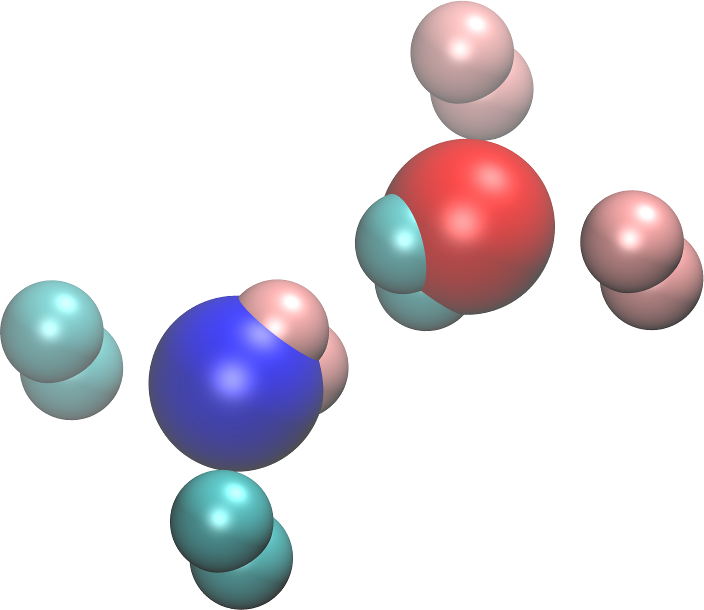
\includegraphics[width=0.45\textwidth]{hires_long_r_crop.png}}%
% FIGURES \fbox{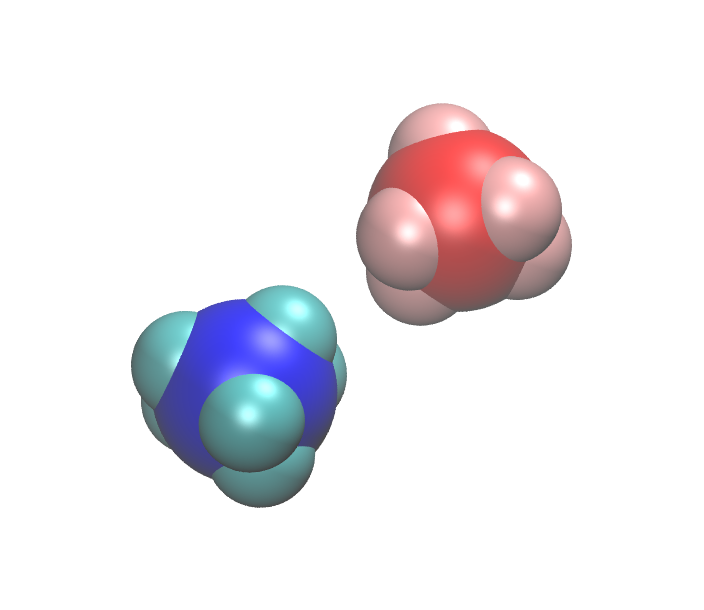
\includegraphics[width=0.45\textwidth]{hires_short_r_crop.png}}
% FIGURES %\caption{Diagrams of pseudo-ethene with \(d =\) 2.0 a.u. (left), and \(d = 0.5\) a.u. (right). The first pseudo-carbon is displayed in blue, with its \(s\) pseudo-potentials in cyan, and the second pseudo-carbon is in red, with its potentials in pink.}
% FIGURES %\label{fig:long_r_ethene}
% FIGURES \end{center}
% FIGURES \vspace{0.25in}
% FIGURES \hspace*{3in}
% FIGURES {\Large
% FIGURES \begin{minipage}[t]{3in}
% FIGURES \baselineskip = .5\baselineskip
% FIGURES Figure 2 \\
% FIGURES Alexander Punter, Paola Nava, Yannick Carissan \\
% FIGURES J.\ Comput.\ Chem.
% FIGURES \end{minipage}
% FIGURES }
% FIGURES 
% FIGURES \clearpage
% FIGURES 
% FIGURES %\vspace*{0.1in}   %%% FIGURE 3
% FIGURES \begin{center}
% FIGURES 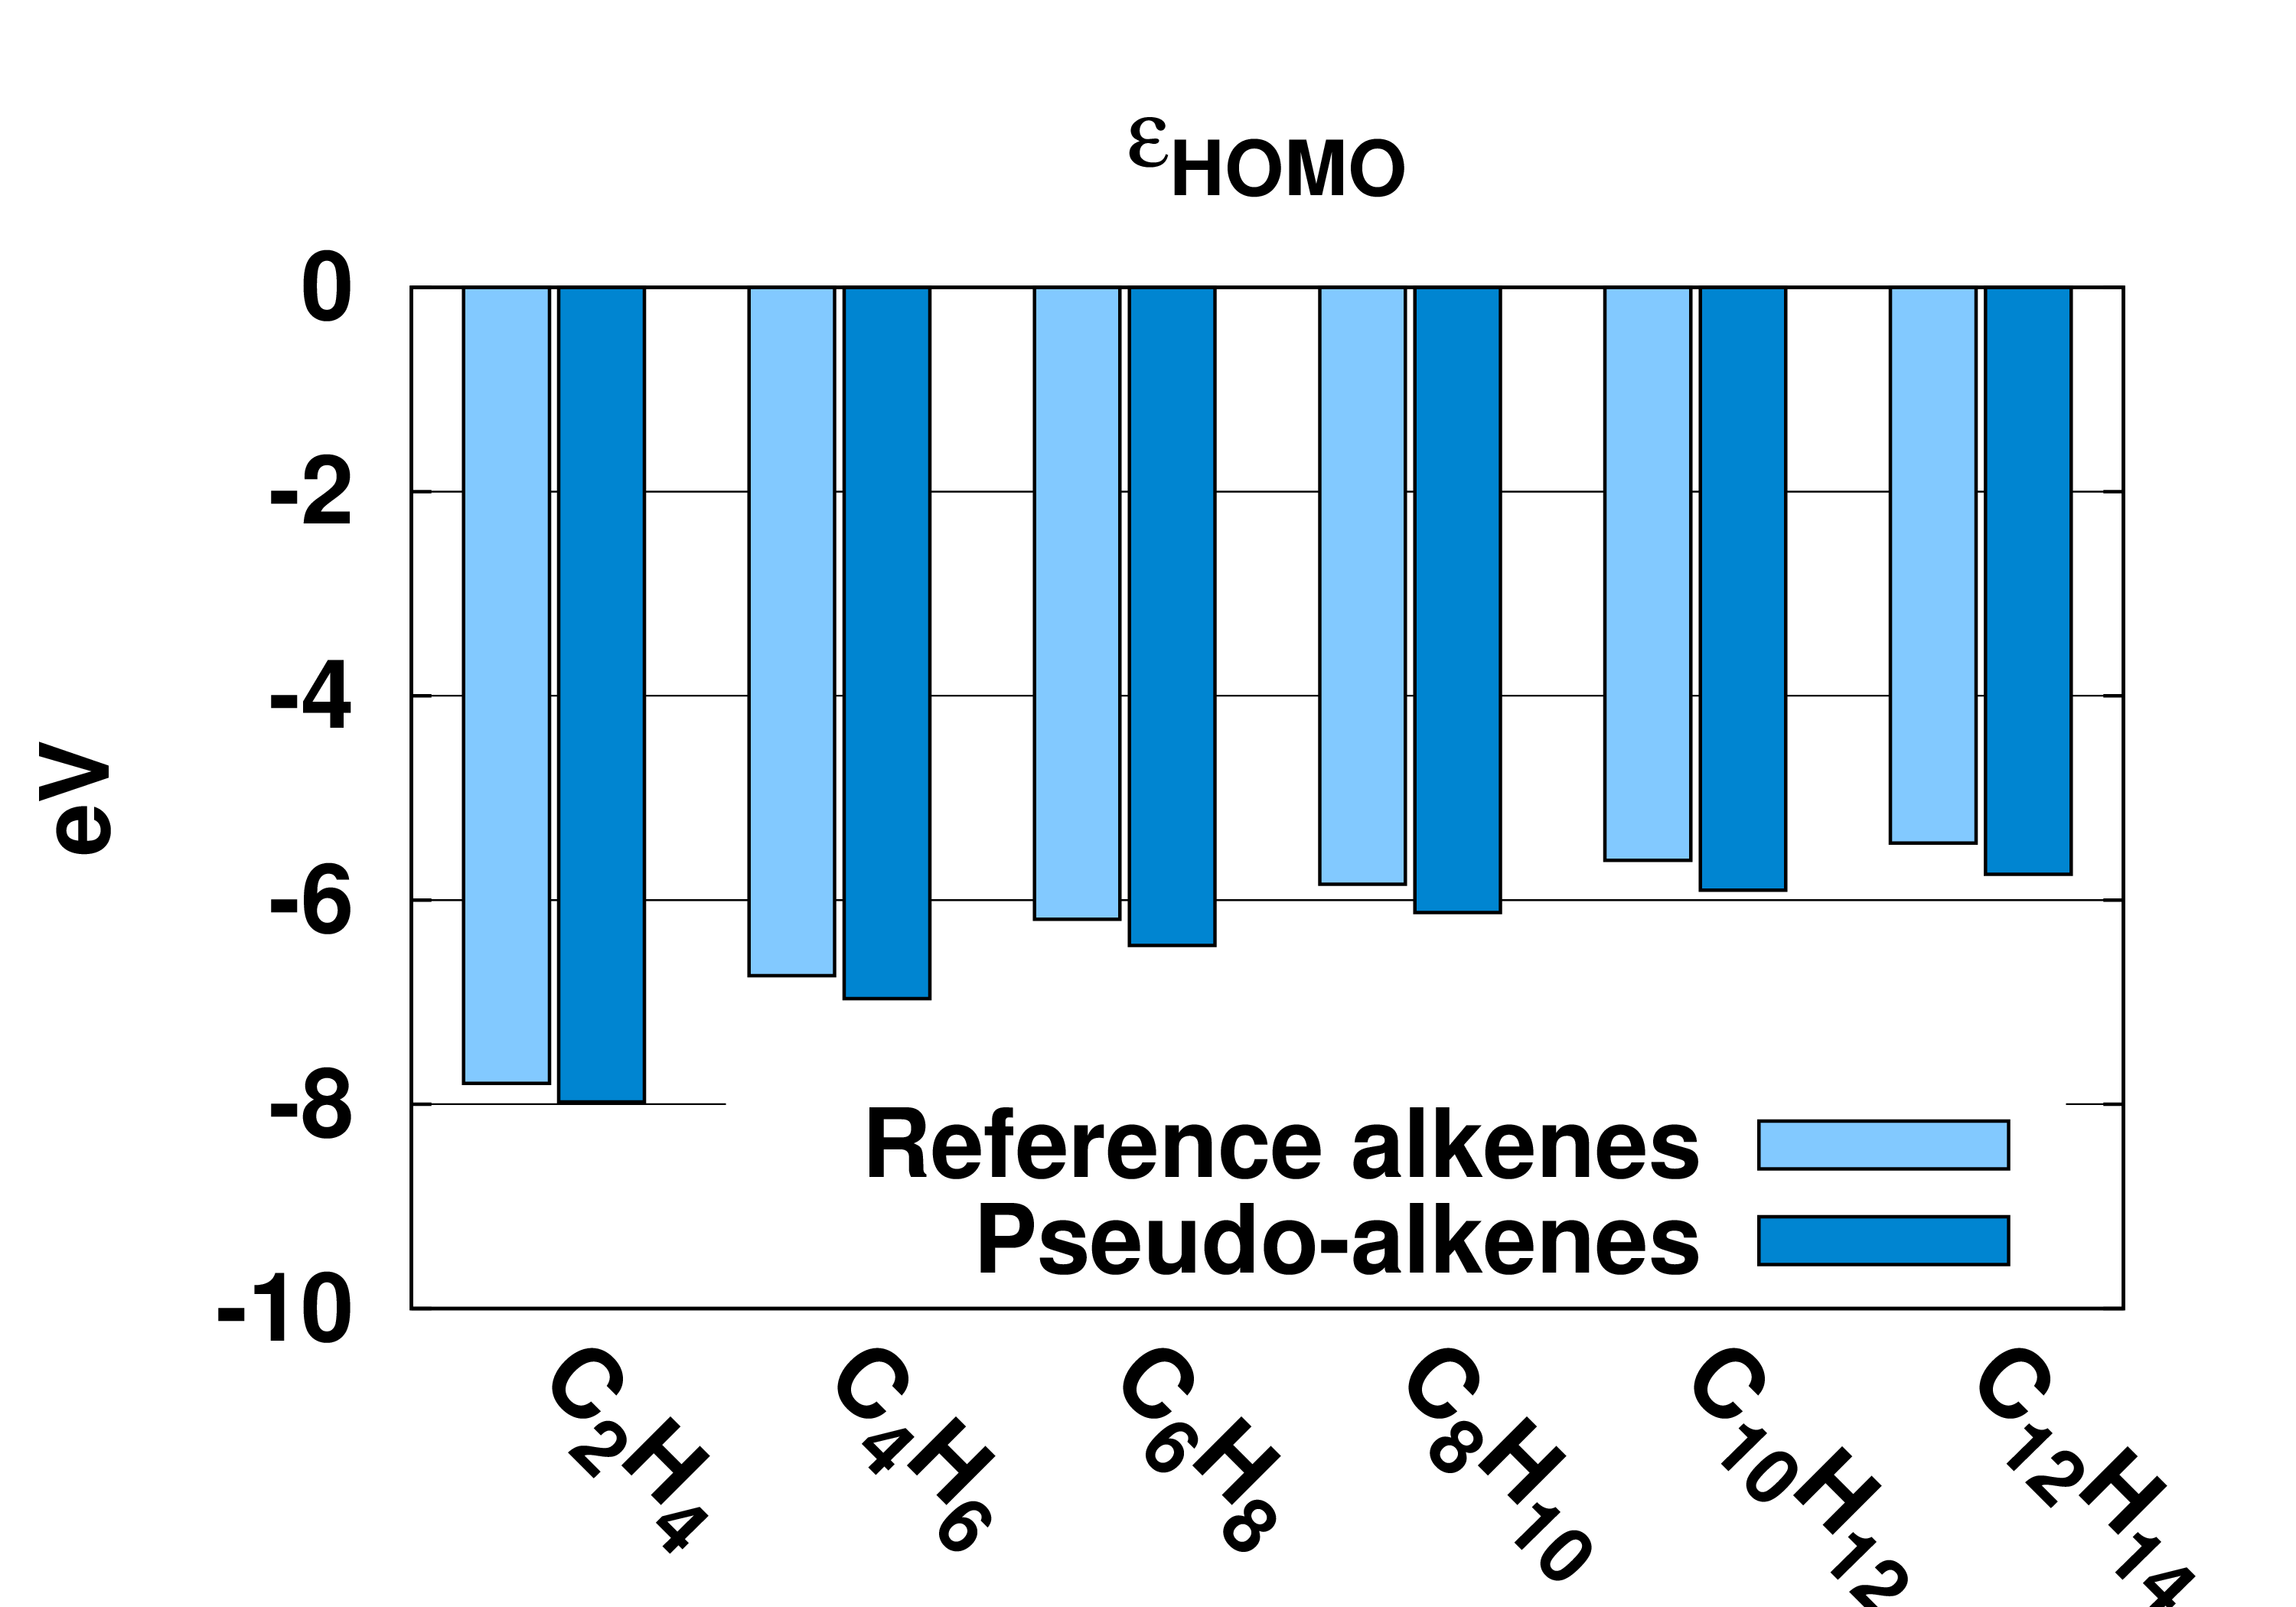
\includegraphics[width=8cm]{short_pbe0_homo}
% FIGURES 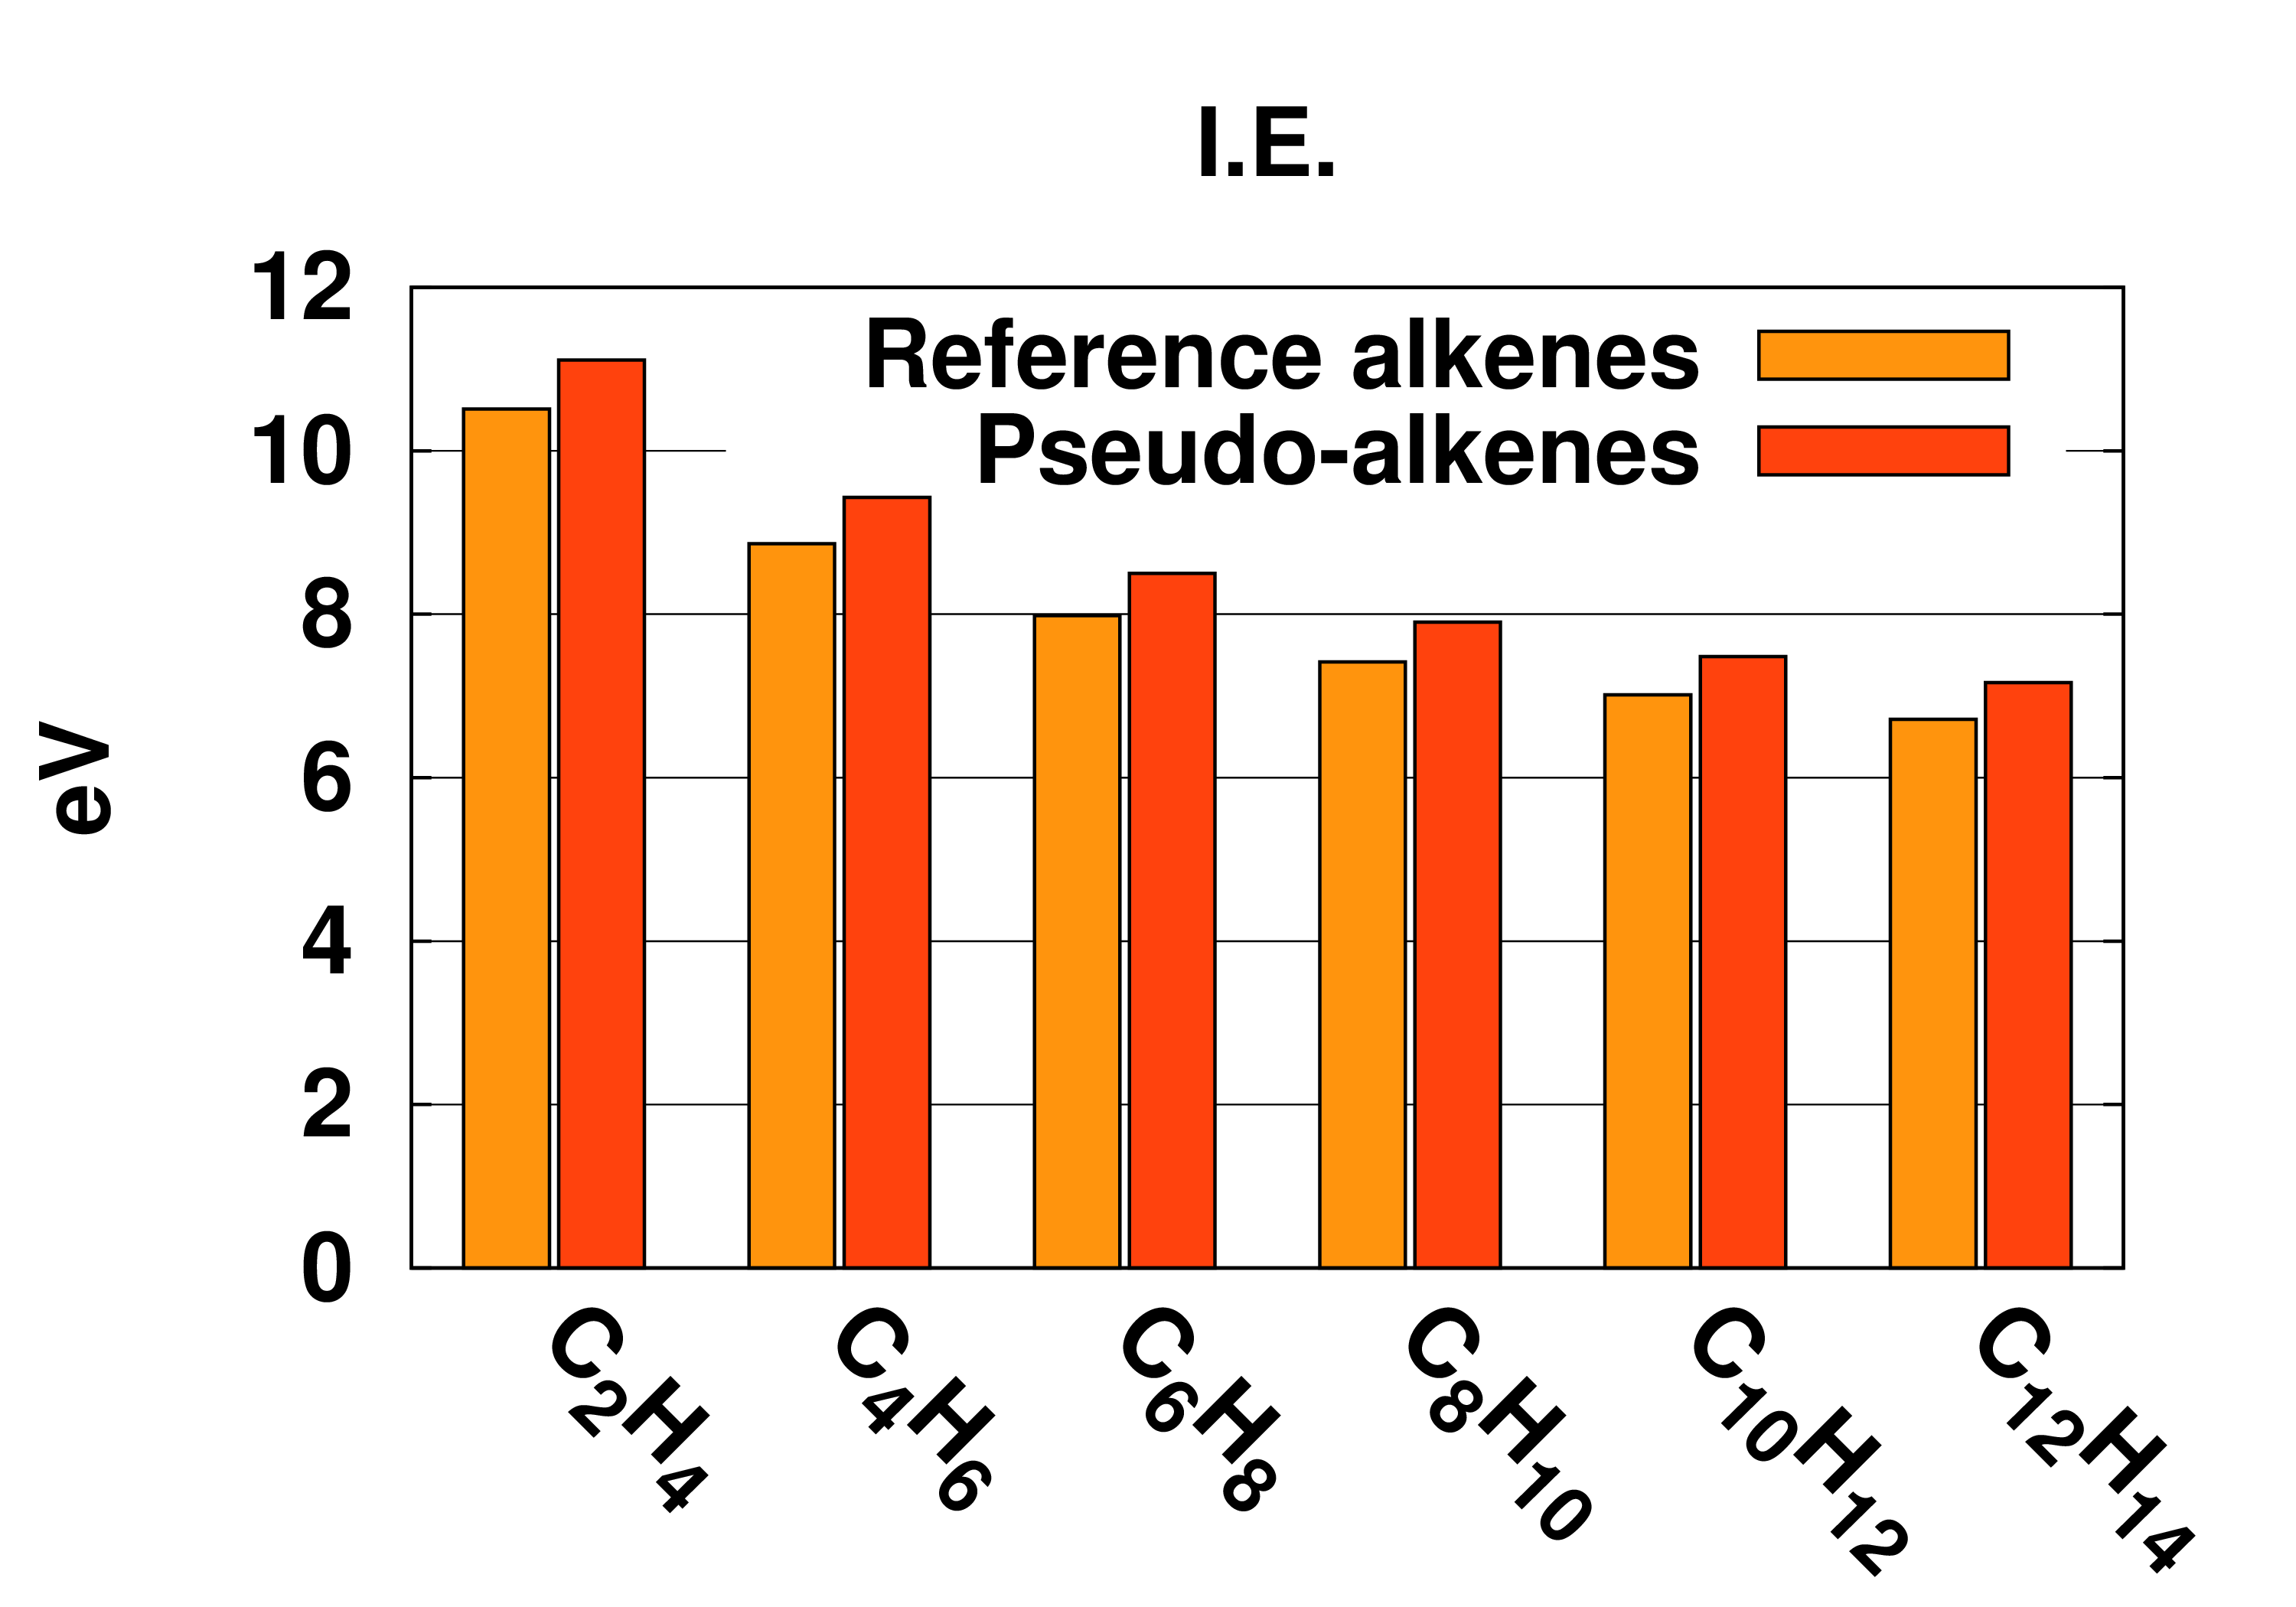
\includegraphics[width=8cm]{short_pbe0_ie}
% FIGURES 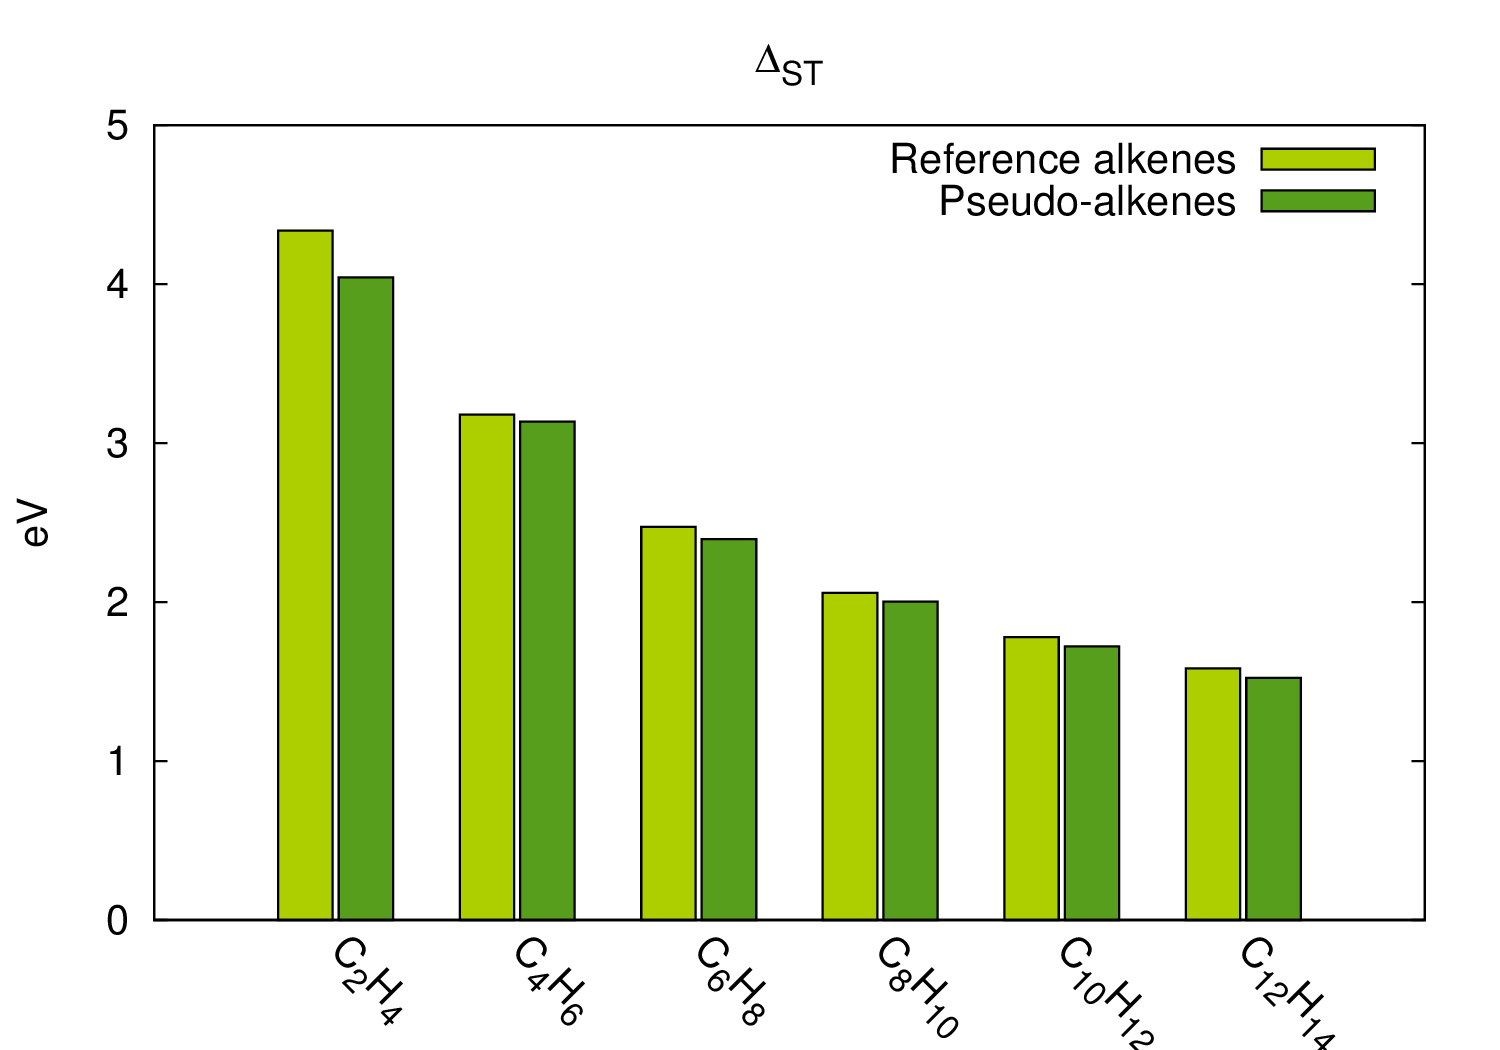
\includegraphics[width=8cm]{short_pbe0_st}
% FIGURES %\caption{DFT (PBE0) comparison of reference and pseudo-system energies across a range of chain alkenes.}
% FIGURES %\label{fig:alkenes_hf_dft}
% FIGURES \end{center}
% FIGURES \vspace{0.25in}
% FIGURES \hspace*{3in}
% FIGURES {\Large
% FIGURES \begin{minipage}[t]{3in}
% FIGURES \baselineskip = .5\baselineskip
% FIGURES Figure 3 \\
% FIGURES Alexander Punter, Paola Nava, Yannick Carissan \\
% FIGURES J.\ Comput.\ Chem.
% FIGURES \end{minipage}
% FIGURES }
% FIGURES 
% FIGURES \clearpage
% FIGURES 
% FIGURES %\vspace*{0.1in}   %%% FIGURE 4
% FIGURES \begin{center}
% FIGURES 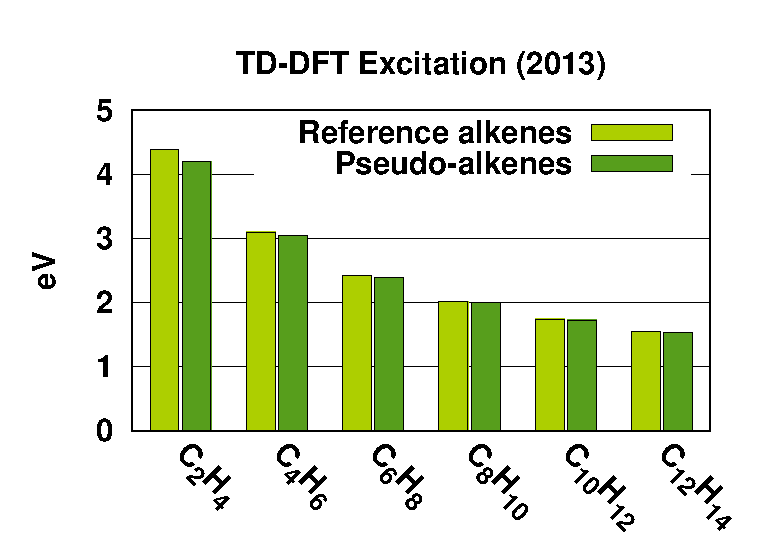
\includegraphics[width=8cm]{short_pbe0_tddft_2013}
% FIGURES 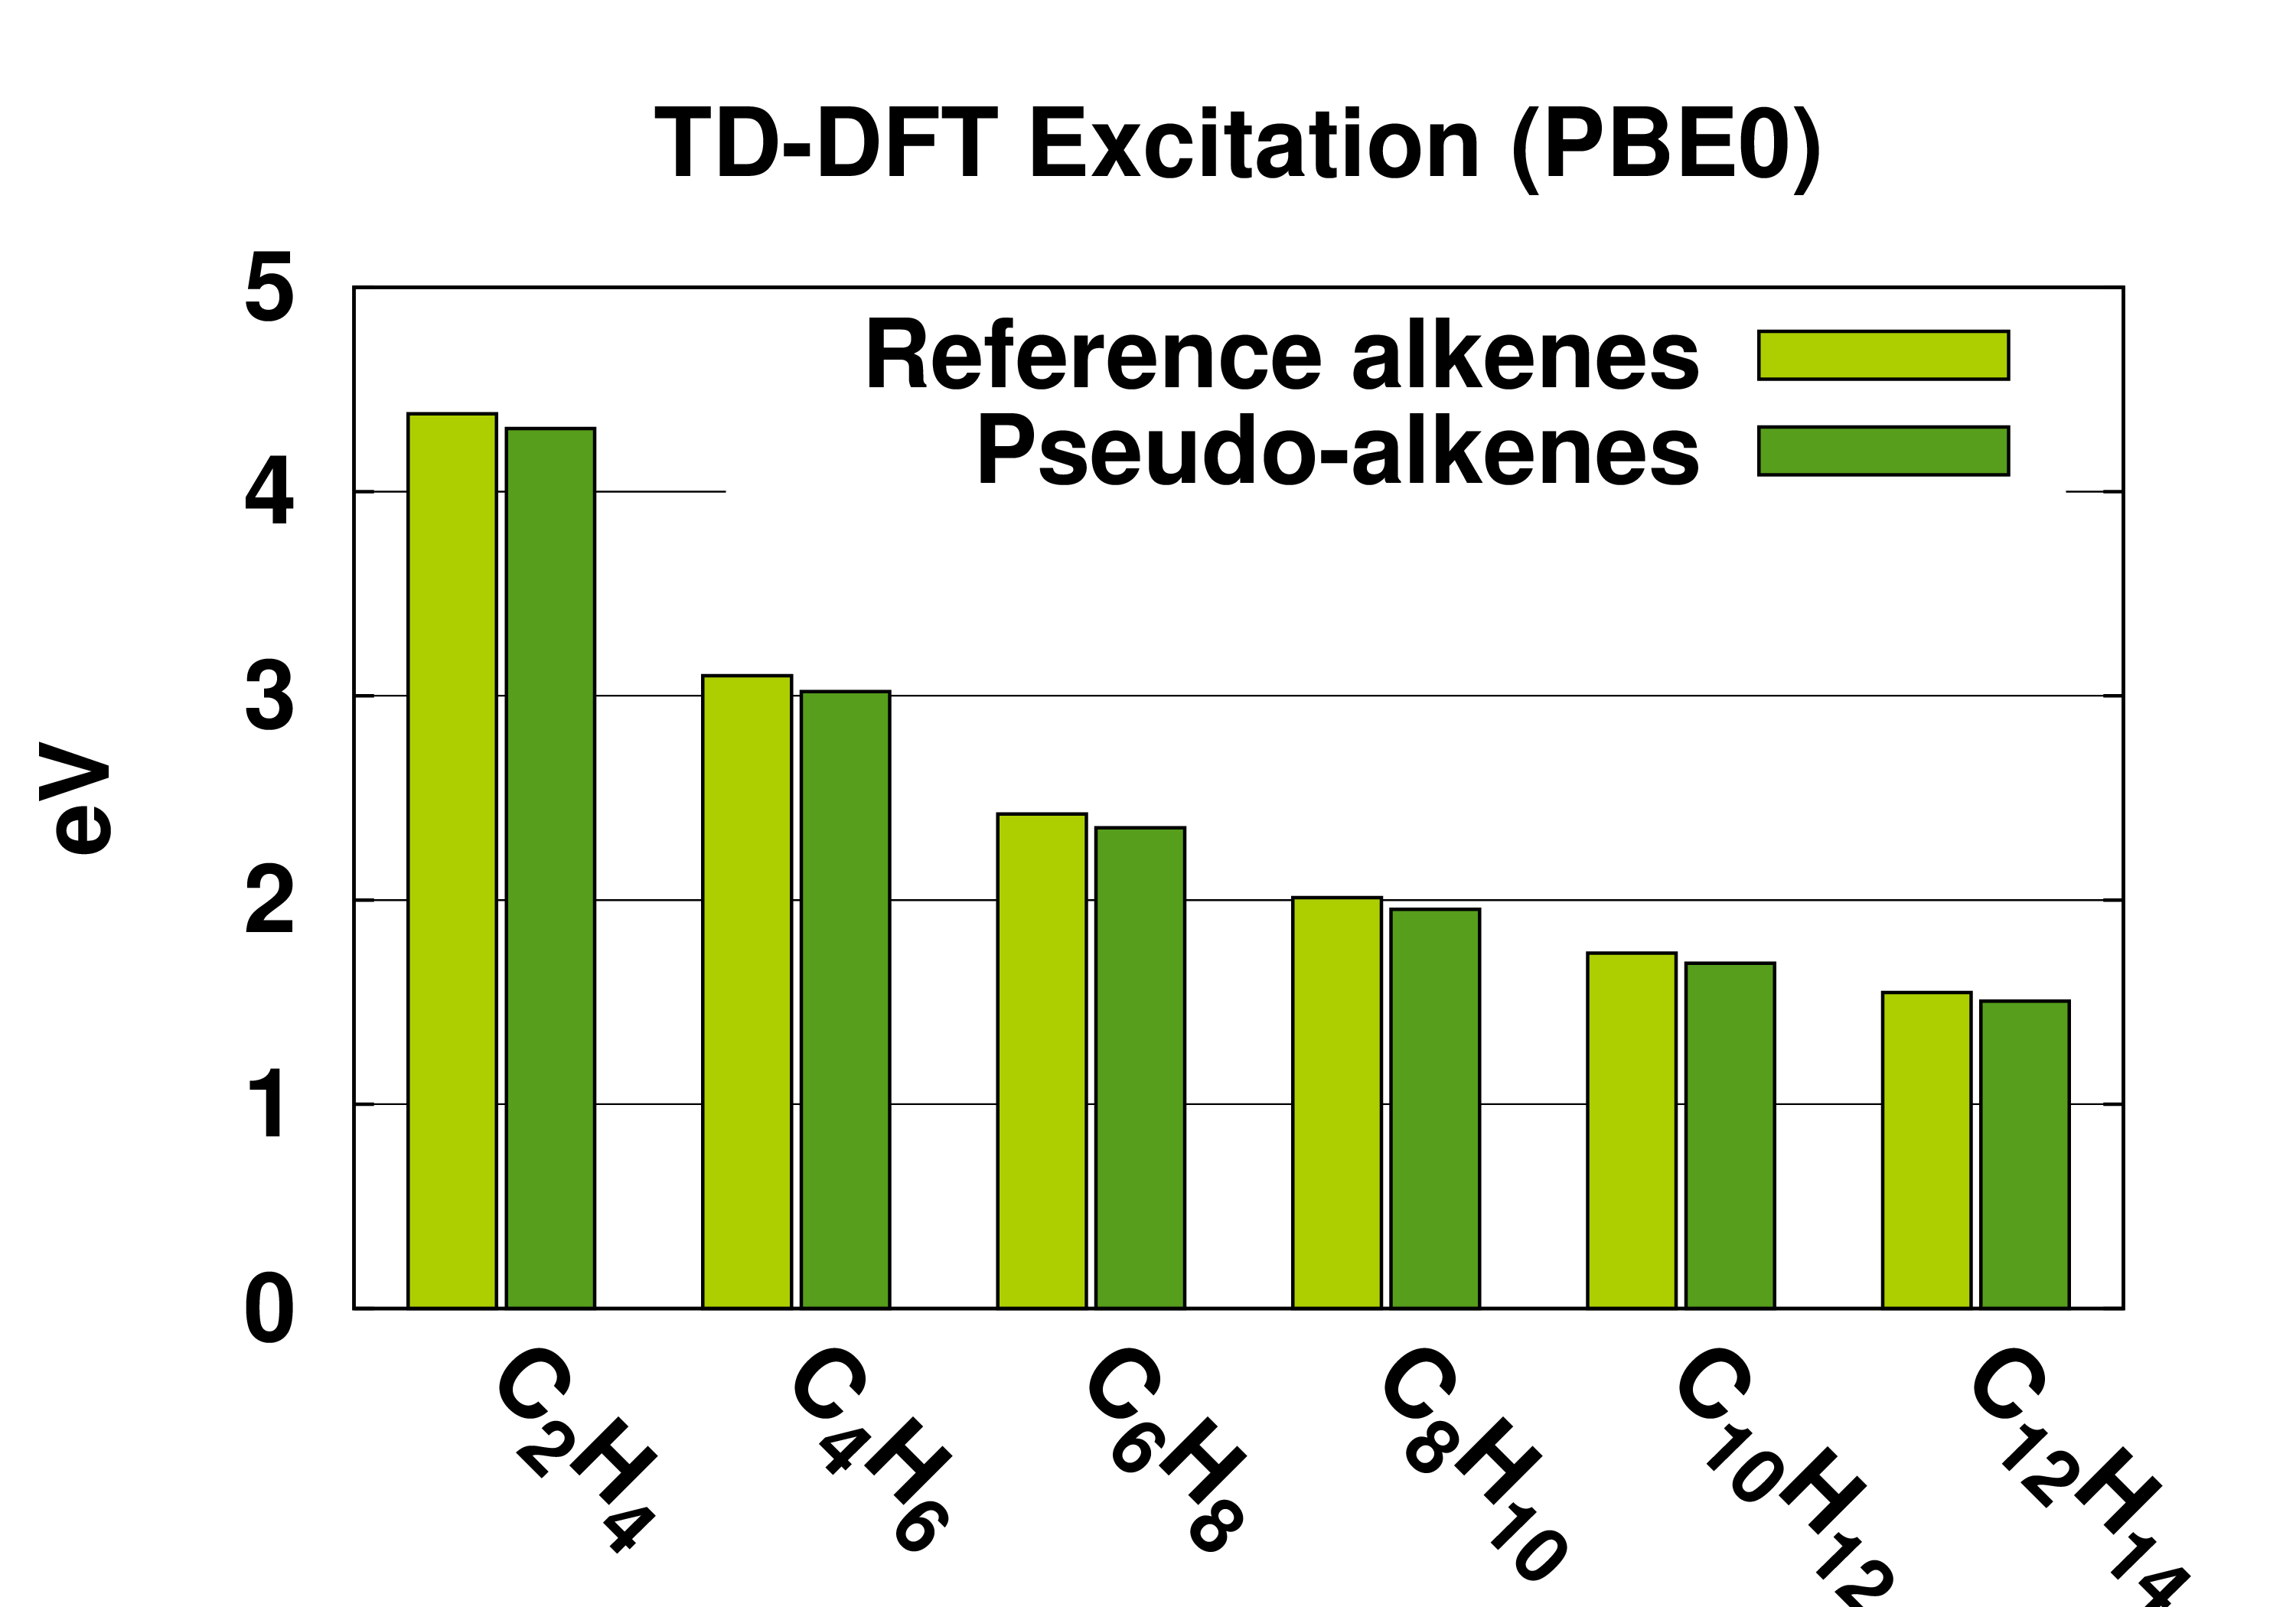
\includegraphics[width=8cm]{short_pbe0_tddft}
% FIGURES %\caption{Comparison of pseudo-alkenes with previous\cite{drujon_pseudopotentials_2013} and current potentials using TD-DFT excitation energies.}
% FIGURES %\label{fig:alkenes_tddft}
% FIGURES \end{center}
% FIGURES \vspace{0.25in}
% FIGURES \hspace*{3in}
% FIGURES {\Large
% FIGURES \begin{minipage}[t]{3in}
% FIGURES \baselineskip = .5\baselineskip
% FIGURES Figure 4 \\
% FIGURES Alexander Punter, Paola Nava, Yannick Carissan \\
% FIGURES J.\ Comput.\ Chem.
% FIGURES \end{minipage}
% FIGURES }
% FIGURES 
% FIGURES \clearpage
% FIGURES 
% FIGURES %\vspace*{0.1in}   %%% FIGURE 5
% FIGURES \begin{center}
% FIGURES 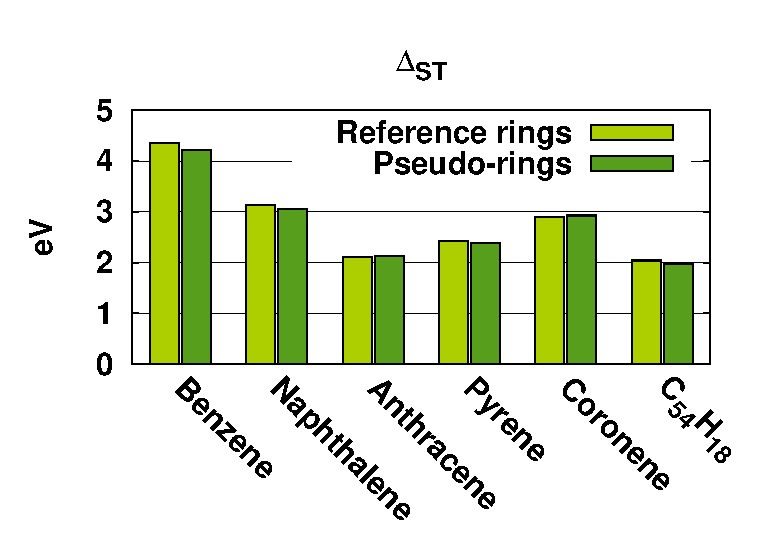
\includegraphics[width=8cm]{ring_pbe0_st}
% FIGURES 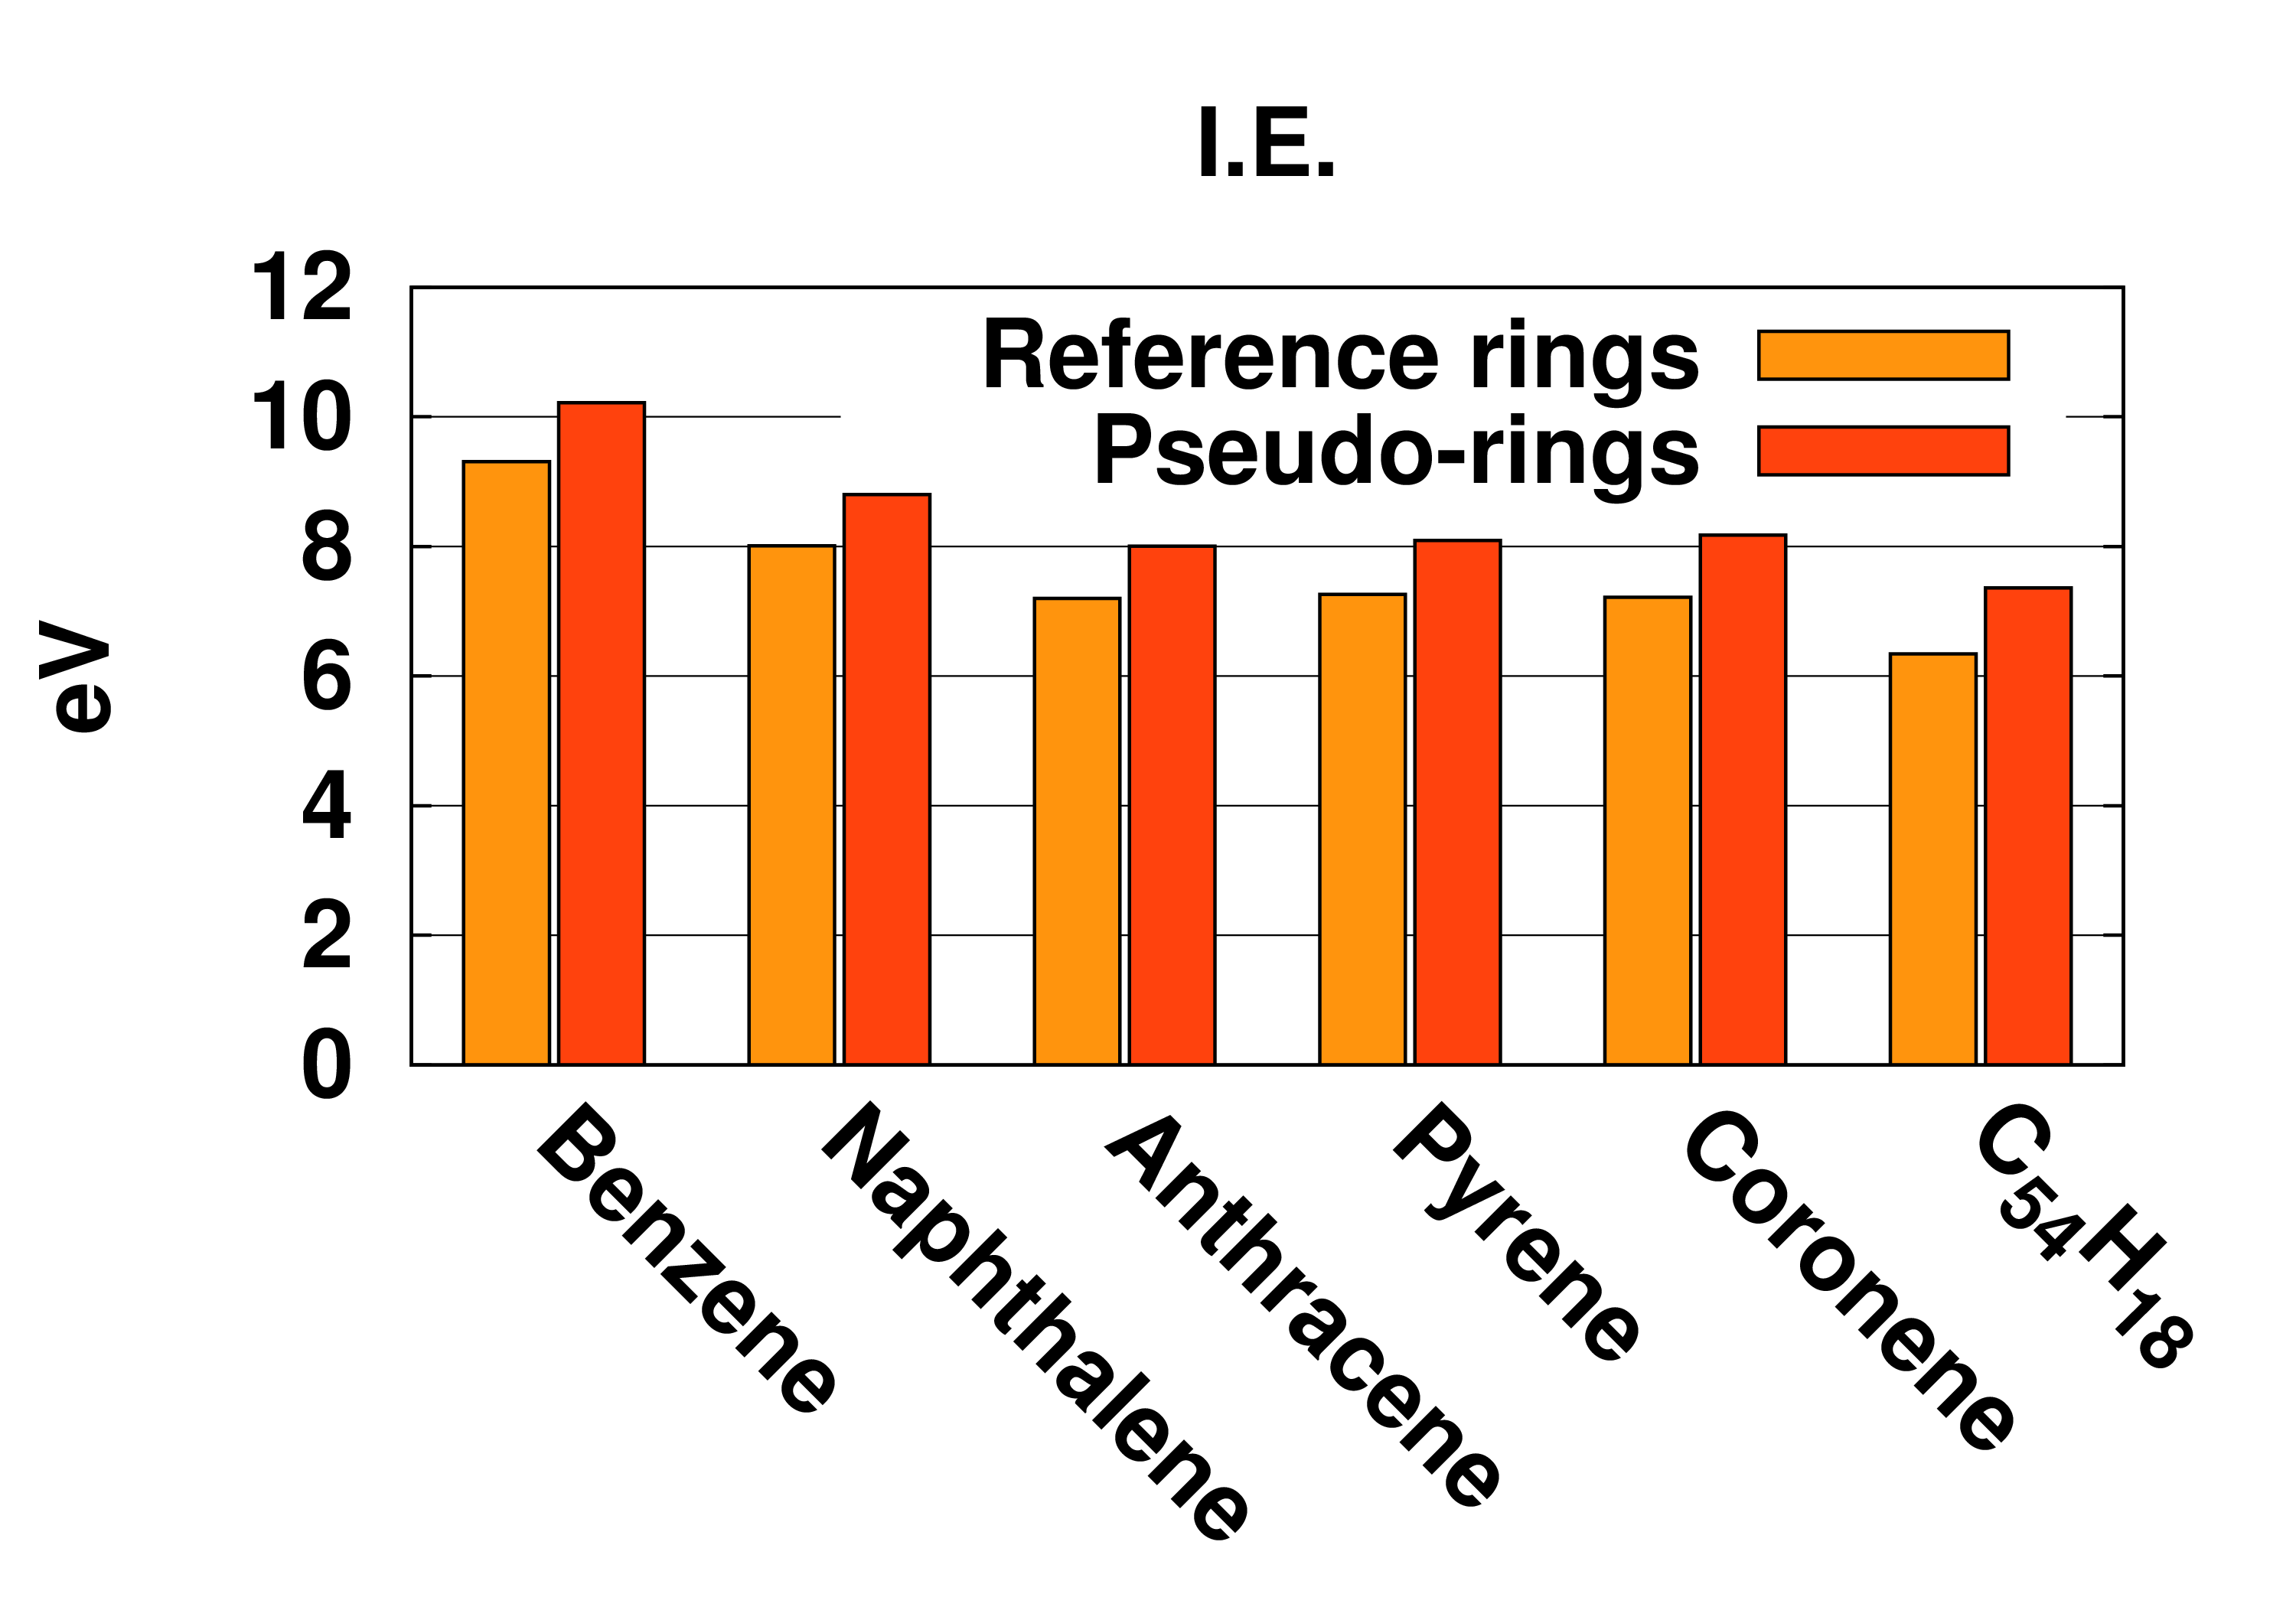
\includegraphics[width=8cm]{ring_pbe0_ie}
% FIGURES 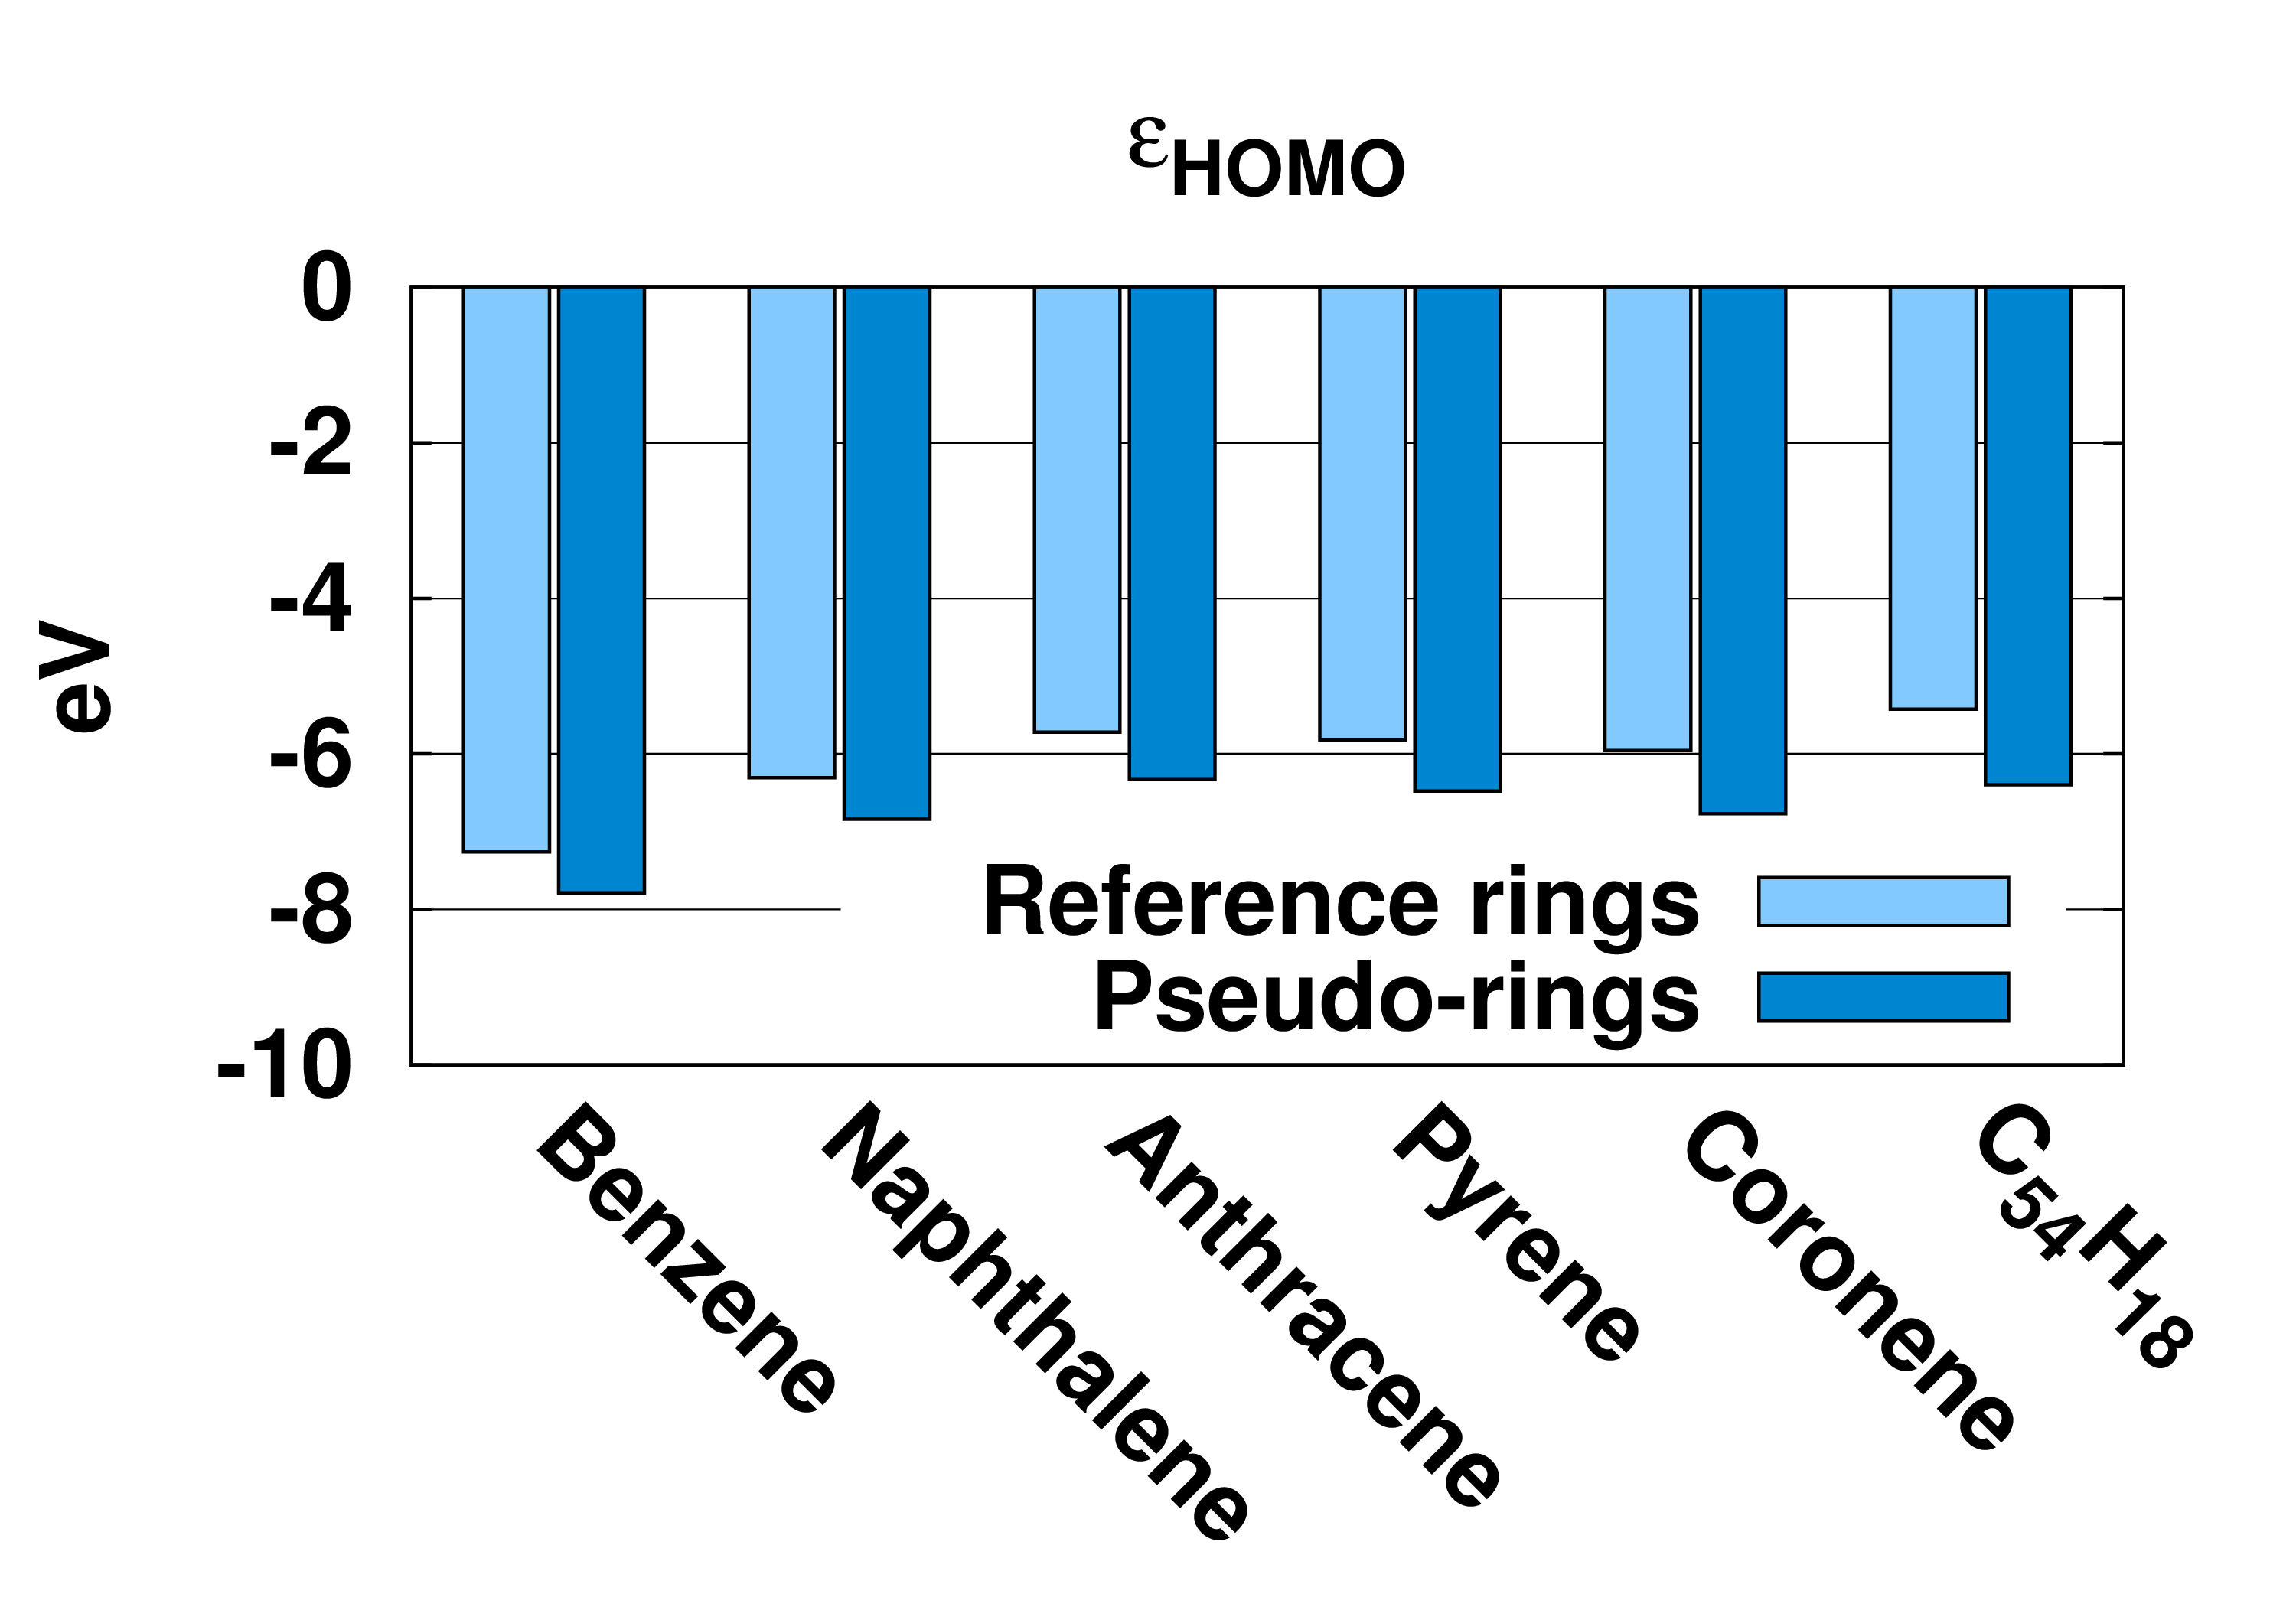
\includegraphics[width=8cm]{ring_pbe0_homo}
% FIGURES 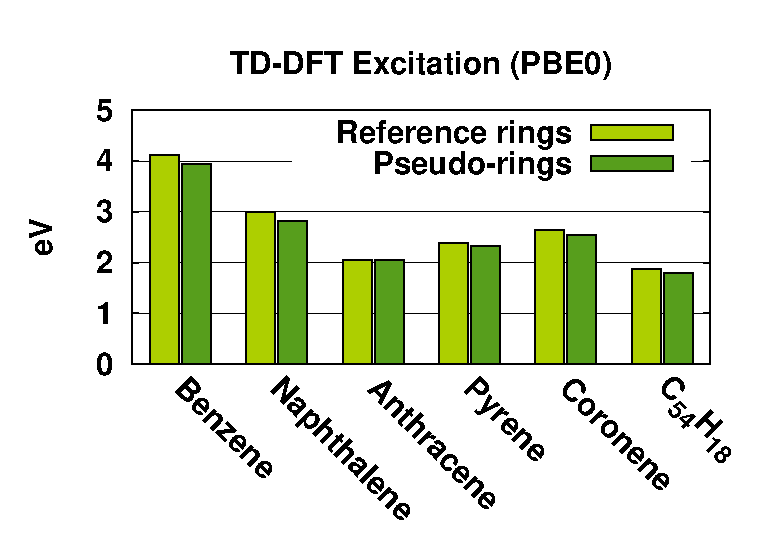
\includegraphics[width=8cm]{ring_pbe0_tddft}
% FIGURES %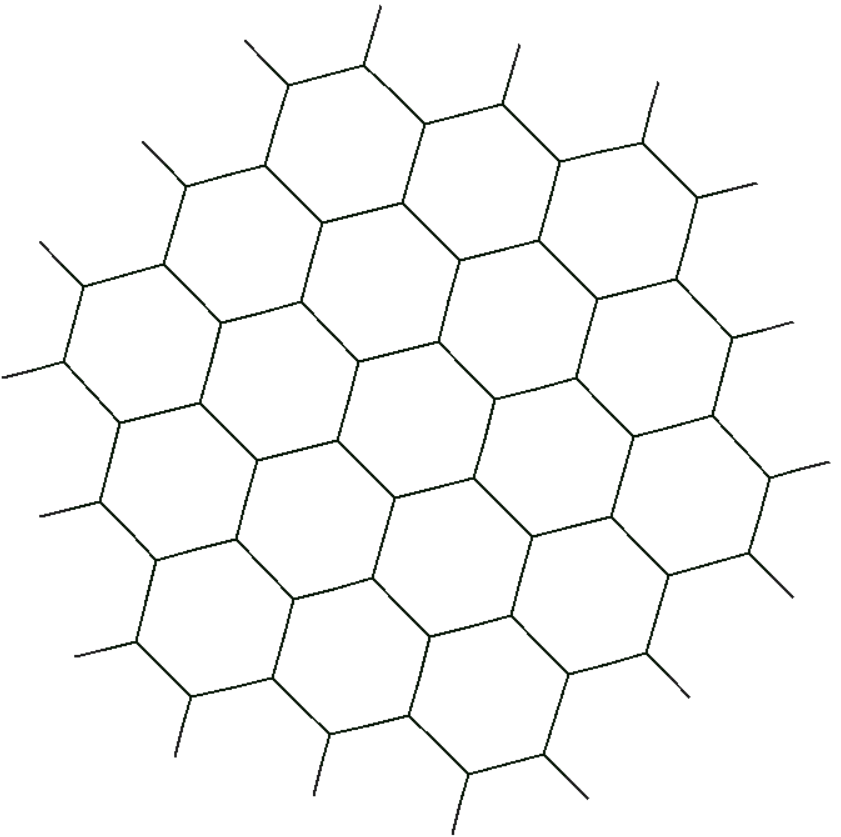
\includegraphics[width=5cm]{19_ring_diagram}
% FIGURES \fbox{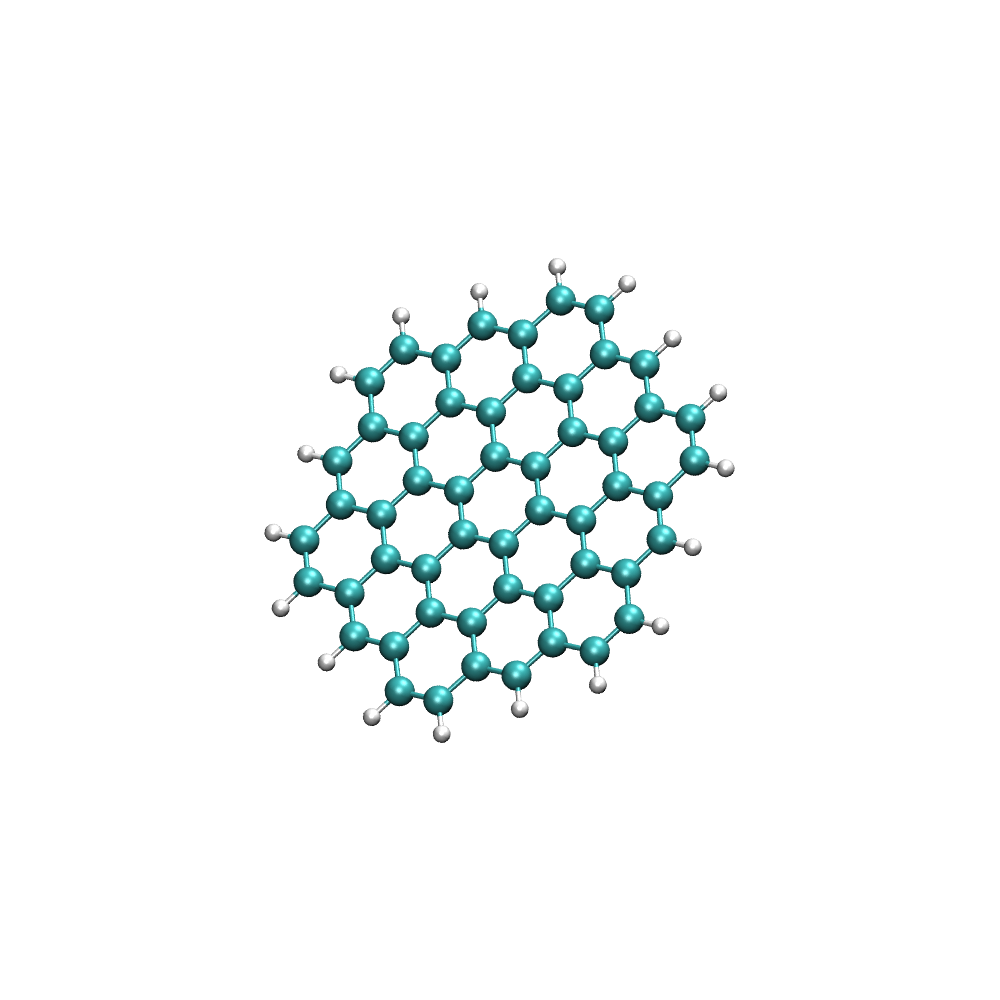
\includegraphics[width=5cm]{c54h18}}
% FIGURES %\caption{DFT and TD-DFT (PBE0) comparison of reference and pseudo-system energies across a range of ring molecules. 
% FIGURES %C\(_{54}\)H\(_{18}\) is shown in the bottom.}
% FIGURES %\label{fig:rings_graphs}
% FIGURES \end{center}
% FIGURES \vspace{0.25in}
% FIGURES \hspace*{3in}
% FIGURES {\Large
% FIGURES \begin{minipage}[t]{3in}
% FIGURES \baselineskip = .5\baselineskip
% FIGURES Figure 5 \\
% FIGURES Alexander Punter, Paola Nava, Yannick Carissan \\
% FIGURES J.\ Comput.\ Chem.
% FIGURES \end{minipage}
% FIGURES }
% FIGURES 
% FIGURES \clearpage
% FIGURES 
% FIGURES %\vspace*{0.1in}   %%% FIGURE 6
% FIGURES \begin{center}
% FIGURES 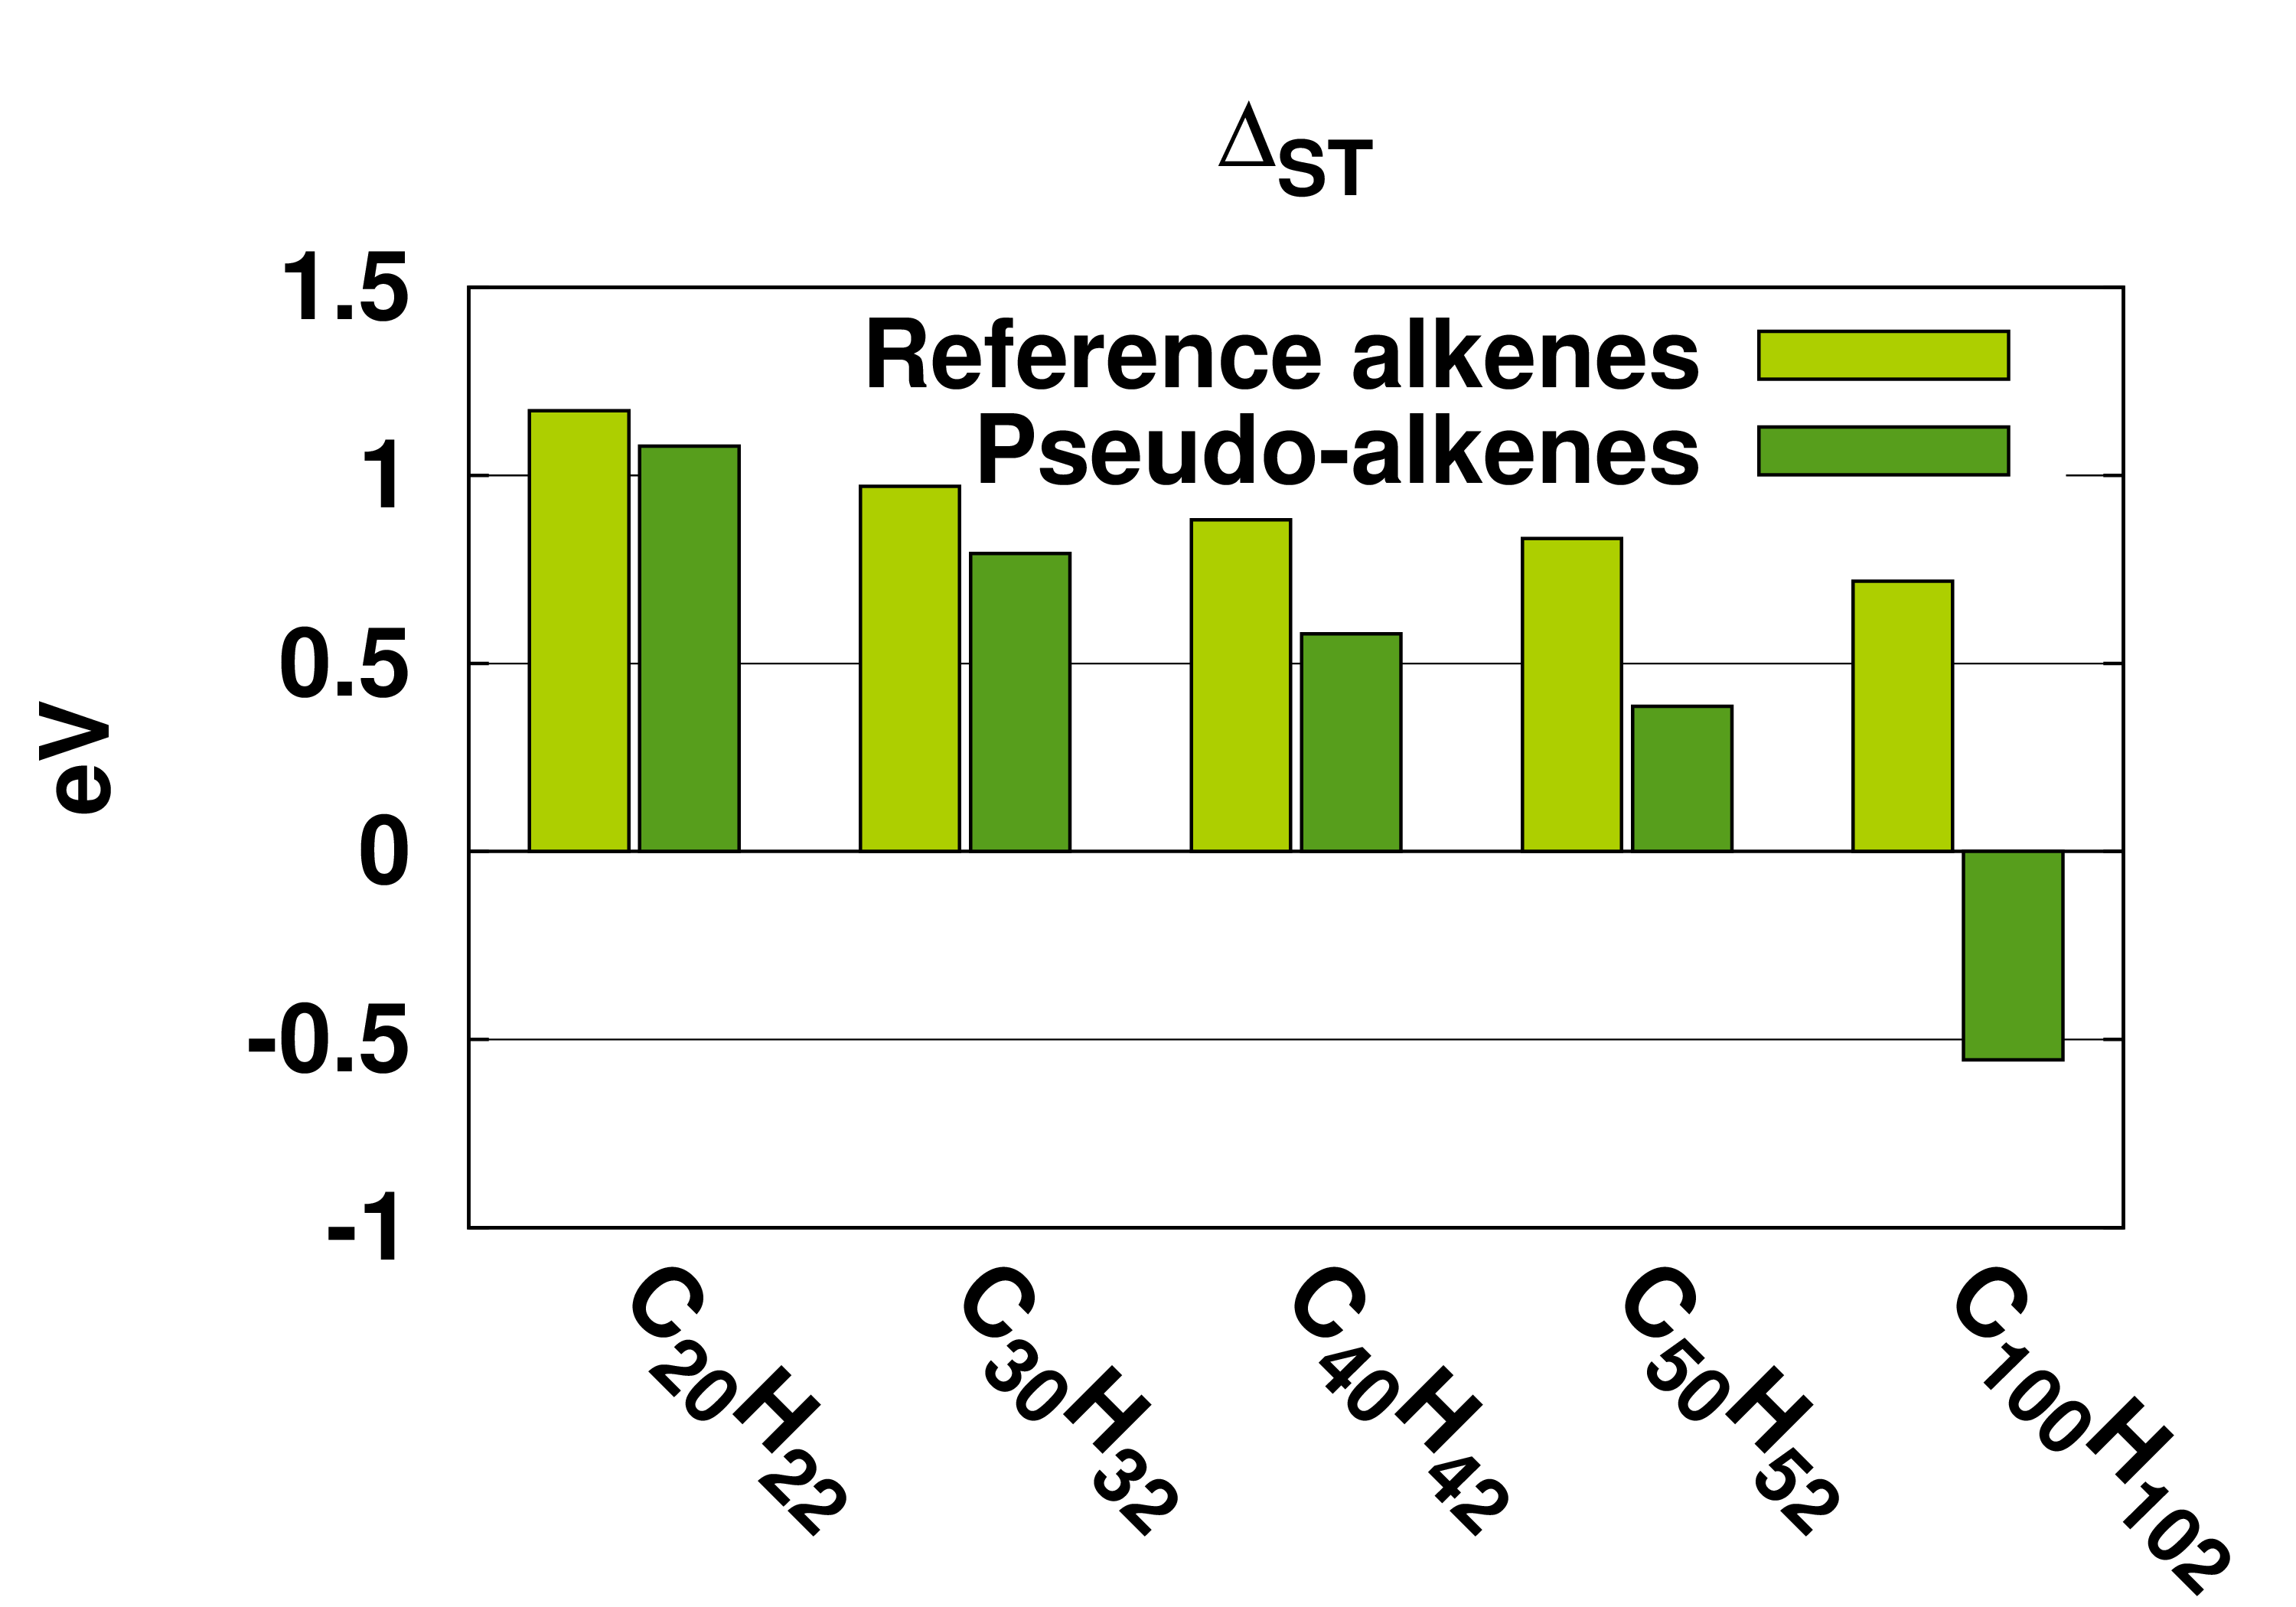
\includegraphics[width=8cm]{long_pbe0_st}
% FIGURES 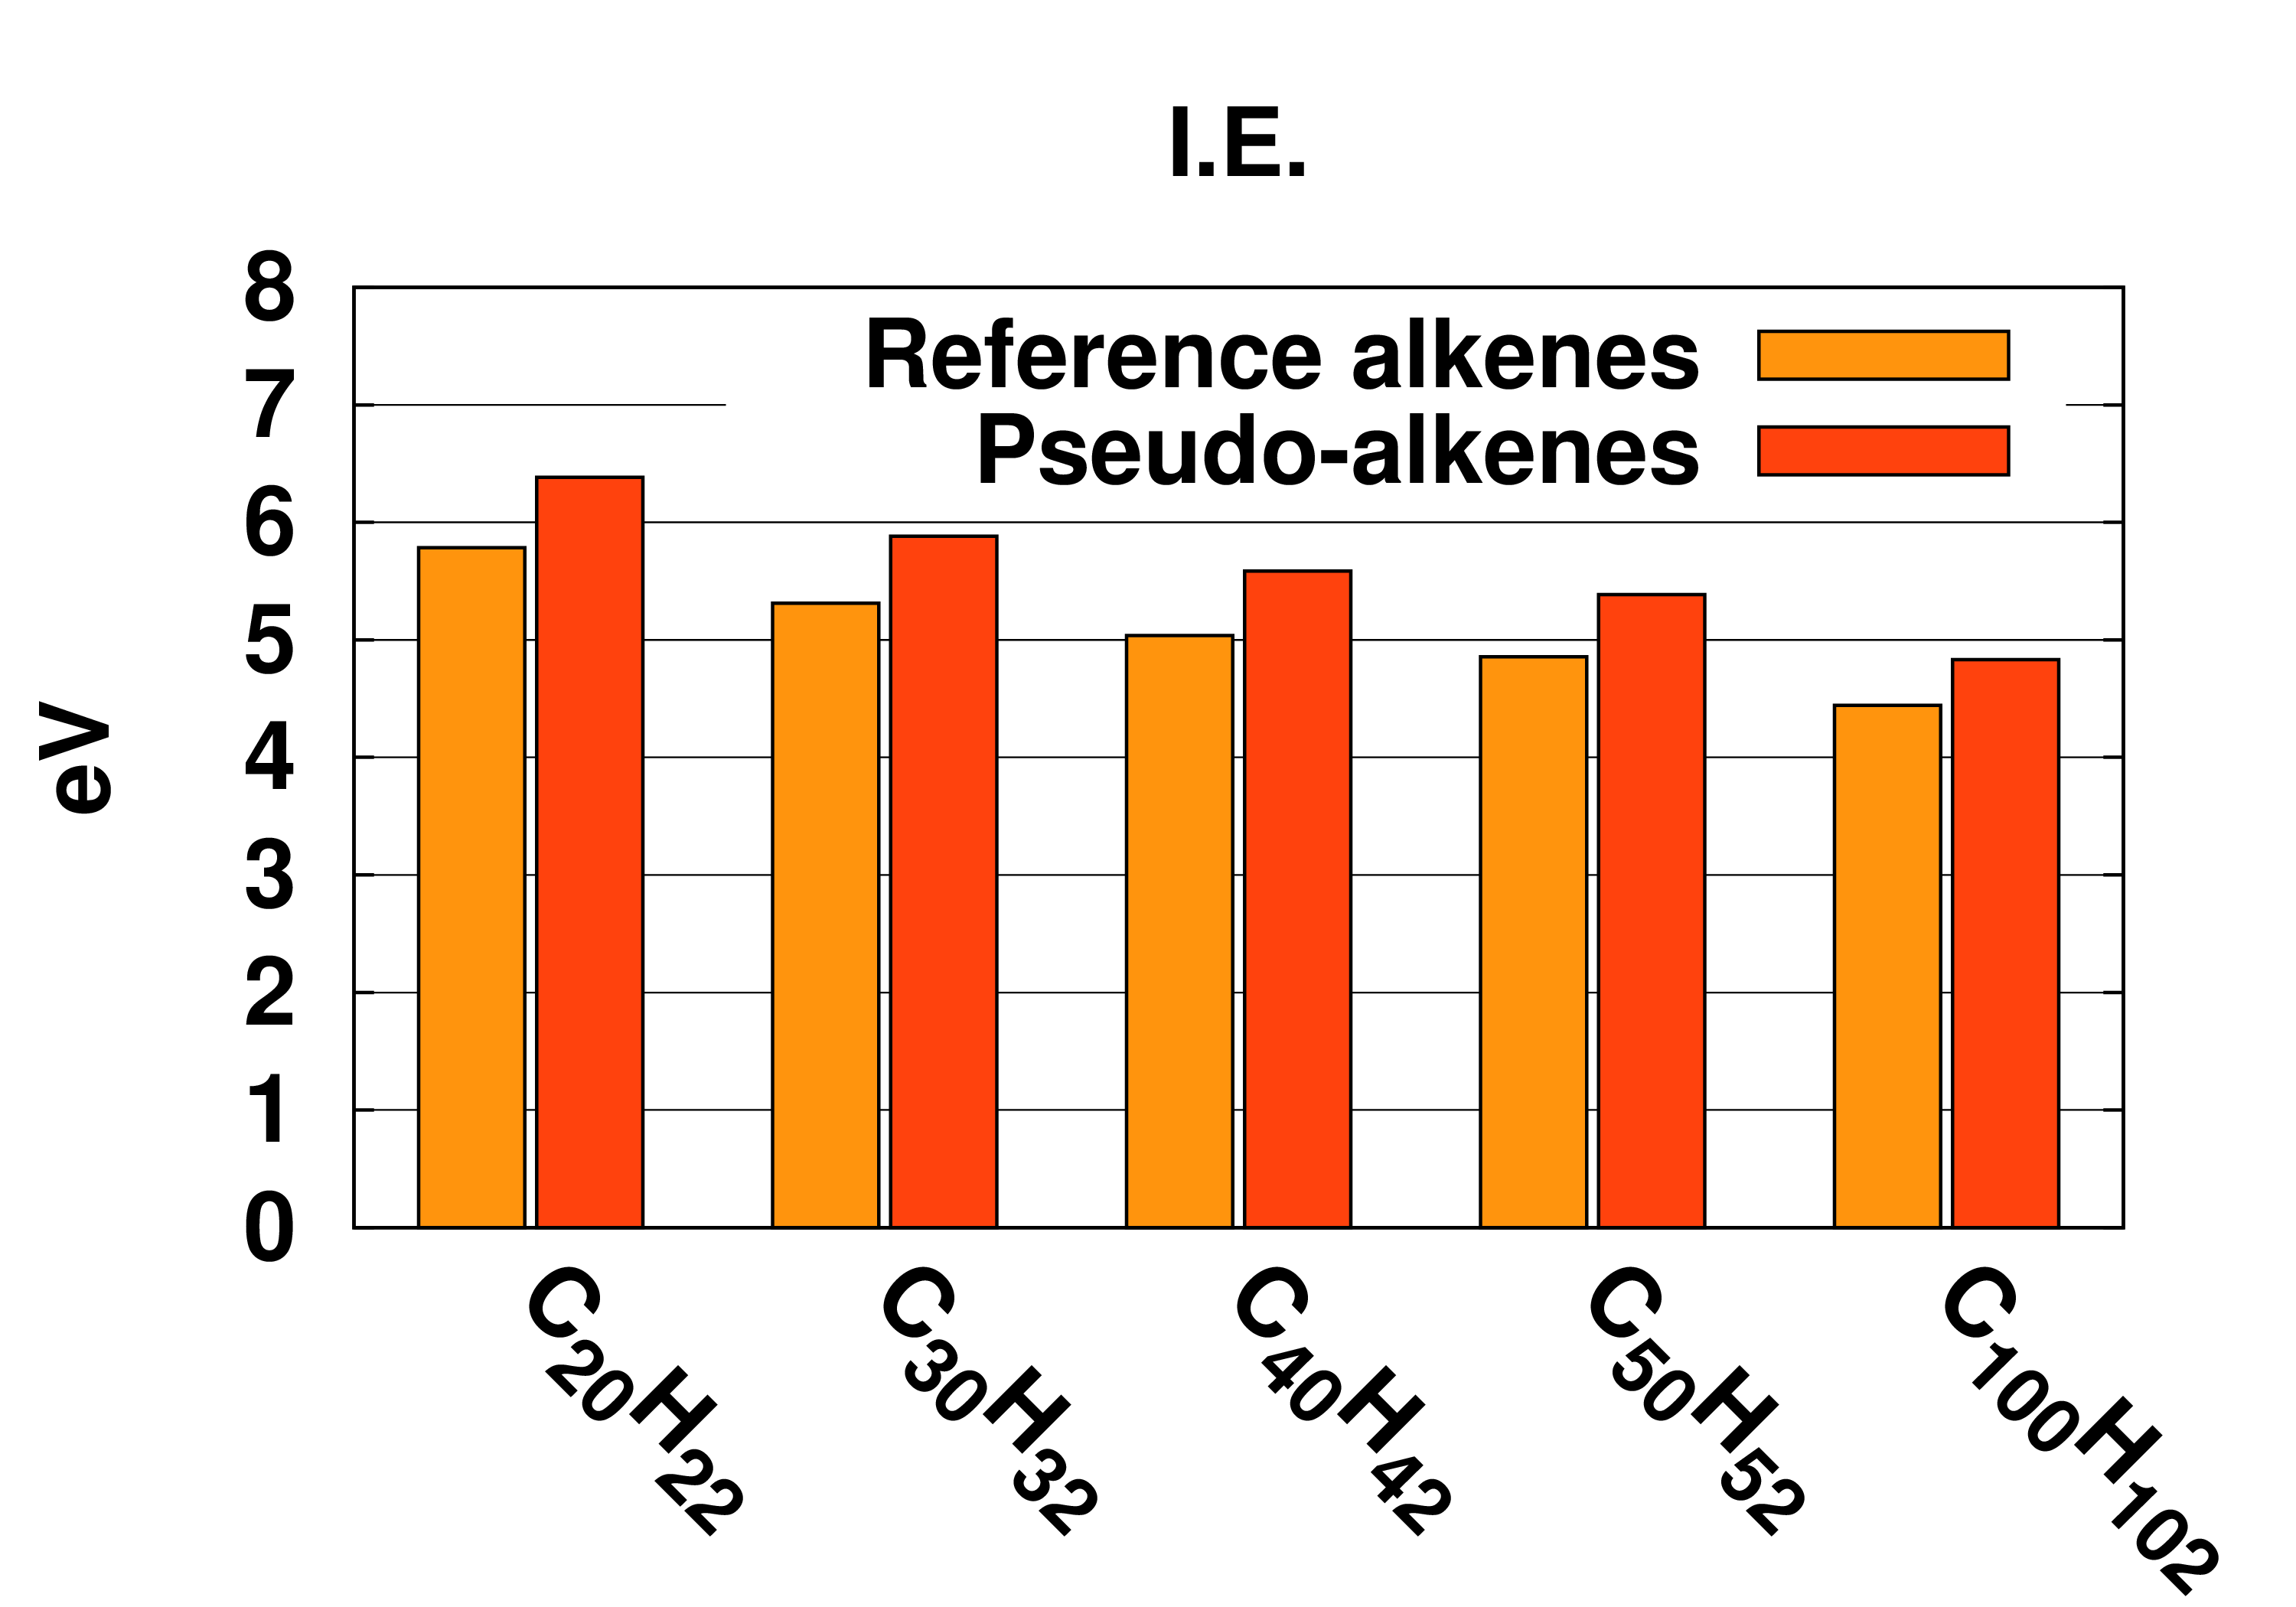
\includegraphics[width=8cm]{long_pbe0_ie}
% FIGURES 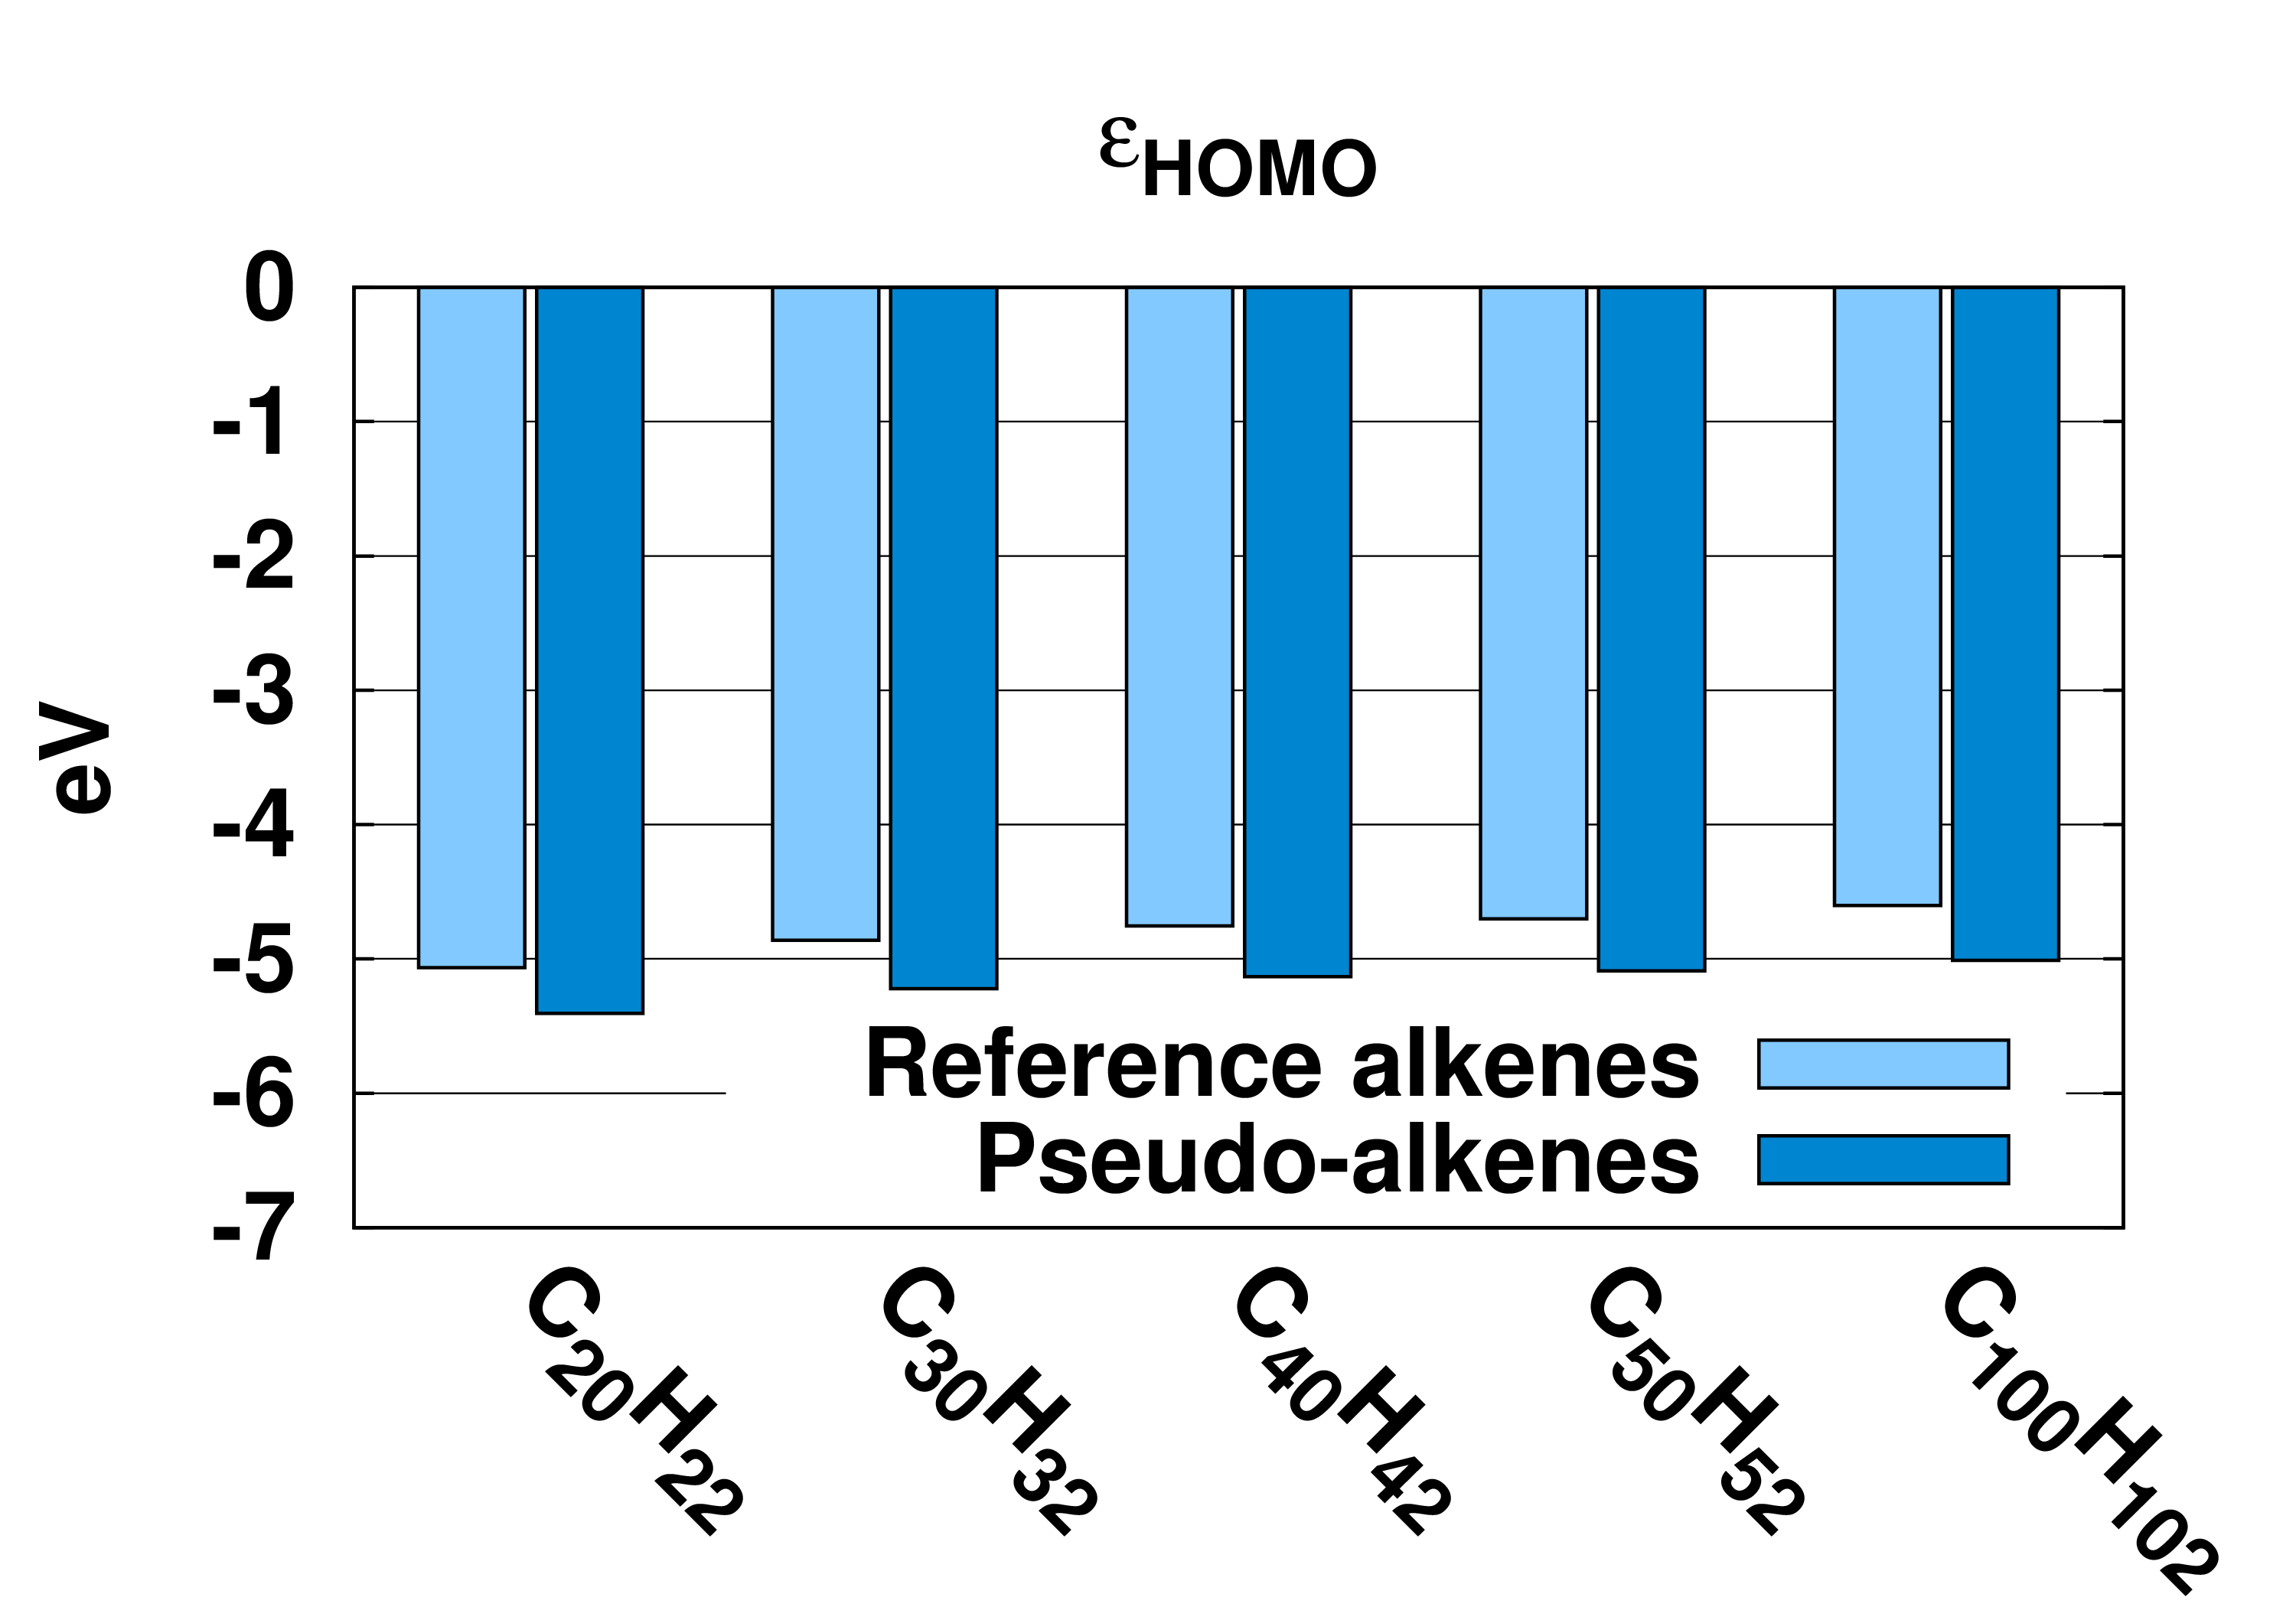
\includegraphics[width=8cm]{long_pbe0_homo}
% FIGURES 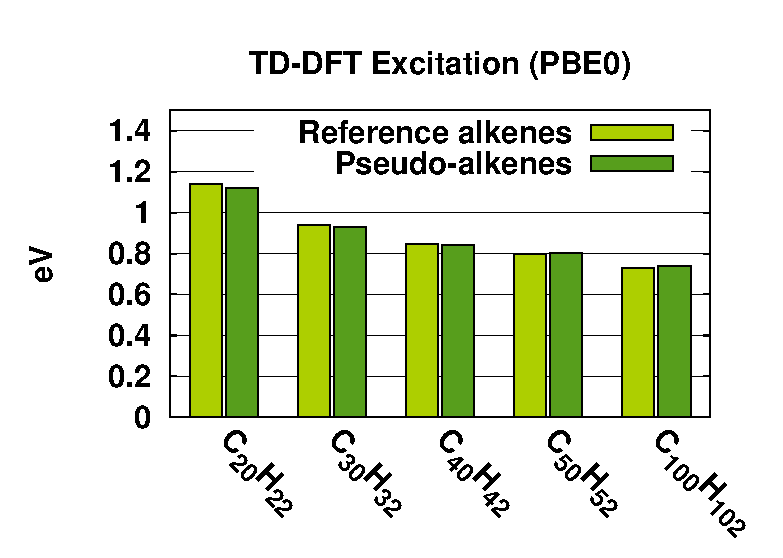
\includegraphics[width=8cm]{long_pbe0_tddft}
% FIGURES %\caption{DFT and TD-DFT (PBE0) comparison of reference and pseudo-system energies across a range of long chain alkenes (C\(_{20}\)-C\(_{100}\)).}
% FIGURES %\label{fig:long_chain_graphs}
% FIGURES \end{center}
% FIGURES \vspace{0.25in}
% FIGURES \hspace*{3in}
% FIGURES {\Large
% FIGURES \begin{minipage}[t]{3in}
% FIGURES \baselineskip = .5\baselineskip
% FIGURES Figure 6 \\
% FIGURES Alexander Punter, Paola Nava, Yannick Carissan \\
% FIGURES J.\ Comput.\ Chem.
% FIGURES \end{minipage}
% FIGURES }
% FIGURES 
% FIGURES \clearpage
% FIGURES 
% FIGURES %\vspace*{0.1in}   %%% FIGURE 7
% FIGURES \begin{center}
% FIGURES 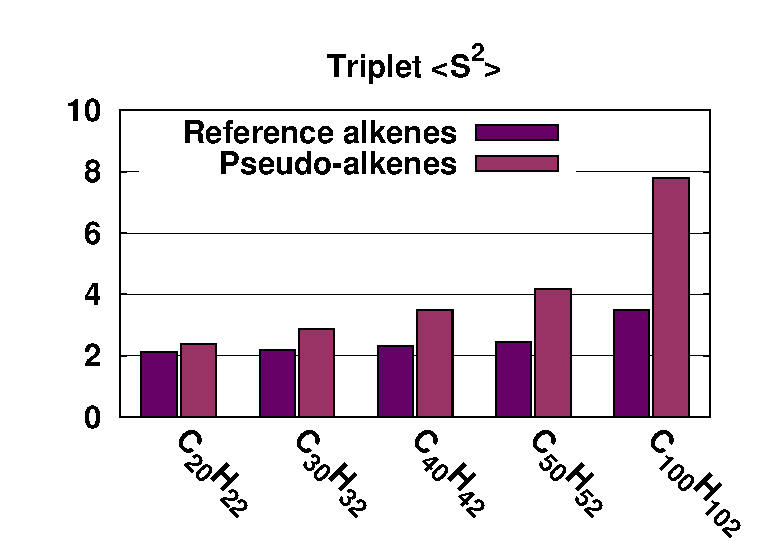
\includegraphics[width=8cm]{long_pbe0_s2}
% FIGURES %\caption{Comparison of $S^2$ expectation values obtained for the calculation
% FIGURES %of the first triplet configuration in a SCF formalism, for reference
% FIGURES %and pseudo-systems.}
% FIGURES %\label{fig:ssquare}
% FIGURES \end{center}
% FIGURES \vspace{0.25in}
% FIGURES \hspace*{3in}
% FIGURES {\Large
% FIGURES \begin{minipage}[t]{3in}
% FIGURES \baselineskip = .5\baselineskip
% FIGURES Figure 7 \\
% FIGURES Alexander Punter, Paola Nava, Yannick Carissan \\
% FIGURES J.\ Comput.\ Chem.
% FIGURES \end{minipage}
% FIGURES }
% FIGURES 
\clearpage
%ENDFIG
%BEGTAB


\begin{table}[h]
\caption{\label{table:potential_params} Comparison of molecular properties of pseudo-CH$^{\bullet}_{3}$ and pseudo-C$_{2}$H$_{4}$ molecules, along with pseudo-potential parameters and reference values.}
\begin{tabular}{c | c c c c | c c c}
\hline
 & \multicolumn{2}{c}{$p$} & \multicolumn{2}{c}{$s$} & \multicolumn{3}{|c}{Energy (eV)} \\
System & coeff. & exp & coeff. & exp. & HOMO & $\Delta_{ST}$ & 1$^{st}$ Ionisation \\
\hline
ref. CH$^{\bullet}_{3}$ & - & - & - & - & -10.537 & - & - \\
ref. C$_{2}$H$_{4}$ & - & - & - & - & -10.363 & -3.522 & -9.091 \\
\hline
initial pseudo-CH$^{\bullet}_{3}$ & -3.268 & 0.295 & 10.381 & 10.000 & -10.537 & - & - \\
initial pseudo-C$_{2}$H$_{4}$ & -3.268 & 0.295 & 10.381 & 10.000 & -14.061 & -9.214 & -14.021\\
\hline
final pseudo-CH$^{\bullet}_{3}$ & -3.910 & 0.624 & 1.500 & 0.500 & -10.000 & - & - \\
final pseudo-C$_{2}$H$_{4}$ & -3.910 & 0.624 & 1.500 & 0.500 & -10.062 & -3.533 & -9.806 \\
\hline
\end{tabular}
\end{table}


\newpage

\begin{table}[h]
\caption{\%-errors across calculation types for short chain alkenes  (C\(_{2}\)-C\(_{12}\))}
\begin{tabular}{c c c c c c }
\hline
Calculation Type & HF & PBE0 & PBE & TPSS & TPSSh \\
\hline
Mean \(\pi - \pi*\) Triplet-Singlet error (\%) & 4.1 & 3.6 & 7.5 & 13.3 & 11.4 \\
Mean Ionisation error (\%) & 5.3 & 6.0 & 8.1 & 10.1 & 9.0 \\
Mean Singlet HOMO error (\%) & 1.3 & 4.0 & 8.5 & 12.0 & 9.7 \\
Mean TD-DFT Excitation error (\%) & - & 2.6 & - & - & - \\ 
\hline
\end{tabular}
\label{table:alkene_errors}
\end{table}

\newpage

\begin{table}[h]
\caption{\%-errors across calculation types for ring-systems}
\begin{tabular}{c c c c c c }
\hline
Calculation Type & HF & PBE0 & PBE & TPSS & TPSSH \\
\hline
Mean \(\pi - \pi*\) Triplet-Singlet error (\%) & 3.3 & 1.9 & 1.7 & 6.8 & 6.7 \\
Mean Ionisation error (\%) & 7.4 & 10.0 & 12.5 & 14.4 & 13.0 \\
Mean Singlet HOMO error (\%) & 3.4  & 9.3  & 13.4 & 17.1 & 14.7 \\
Mean TD-DFT Excitation error (\%) & - & 0.099 & - & - & - \\ 
\hline
\end{tabular}
\label{table:ring_system_errors}
\end{table}

\newpage

\begin{table}[h]
\caption{\%-errors across calculation types for long chain alkenes (C\(_{20}\)-C\(_{100}\))}
\begin{tabular}{c c c c c c }
\hline
Calculation Type & HF & PBE0 & PBE & TPSS & TPSSH \\
\hline
Mean \(\pi - \pi*\) Triplet-Singlet error (\%) & 55.3 & 85.8 & 83.4 & 239.8 & 320.2 \\
Mean Ionisation error (\%) & 25.1 & 6.7 & 9.4 & 10.3 & 11.6 \\
Mean Singlet HOMO error (\%) & 1.8 & 7.3 & 11.3 & 16.7 & 13.6 \\
Mean TD-DFT Excitation error (\%) & - & 0.005 & - & - & - \\ 
\hline
\end{tabular}
\label{table:long_alkene_errors}
\end{table}

\newpage

\begin{table}
\caption{\label{tab:coef}Comparison of the weights (all electron \emph{vs.} pseudo-potentials)
of the excitations obtained with TD-DFT
to represent the triplet excited state from the closed shell singlet state.
Example case of C$_{50}$H$_{52}$.}
\begin{tabular}{c c c c}
\hline
\multicolumn{2}{c}{Excitation} & \multicolumn{2}{c}{Weight(\%)}\\
\multicolumn{2}{c}{MO} & Ref. & Pseudo.\\
\hline
\multicolumn{2}{c}{25 a" \(\rightarrow\) 26 a"} & 77.0 &   67.1  \\
\multicolumn{2}{c}{24 a" \(\rightarrow\) 27 a"} & 10.5 &   13.1  \\
\multicolumn{2}{c}{23 a" \(\rightarrow\) 28 a"} & 3.6  &    5.2  \\
\hline
\end{tabular}
\end{table}
%ENDTAB

\begin{table}[ht]
\caption{\label{tab:time}Time (in seconds) per SCF iteration and relative
gain (time ratio all-electron/pseudo-potential) for a standard and a large basis set.} 
\begin{tabular}{lrr}
\hline\hline
Model            & def2-SV(P) & QZVPPD \\
\hline
All electrons    &        67 & 68928 \\
Pseudo-potential &        28 &  8566 \\
Gain (no unit)   &       2.4 &   8.0 \\
\hline\hline
\end{tabular}
\end{table}

\end{document}

